\chapter{Results and Discussion}
\label{ch:results}
The research process resulted in numerous interesting findings, with implications both for understanding the behavior of the system, as well as for future design efforts considering multi-spacecraft surveys. These results will be presented and discussed in this chapter. Firstly, the system's orbital elements, and how these are affected by the composition of the system, will be discussed in \autoref{sec:results_orbits_one} for spacecraft in co-orbital configurations. Afterwards, the effect of increasing or decreasing the number of spacecraft is discussed in \autoref{sec:results_number}. Then, possible payload compositions are assessed in \autoref{sec:results_payload}. To aid in the interpretation of these results, a possible explanation for the underlying principle is presented in \autoref{sec:results_explanation}. \autoref{sec:results_orbits_two} extends the analysis of the orbital parameters to non-co-orbital configurations, supported by the hypotheses on the underlying principles. Finishing the discussion, in \autoref{sec:results_performance}, predictions will be made with respect to the performance of an optimal multi-spacecraft survey system, and the impact on future design efforts will be discussed.


\section{Orbital Elements I: Co-orbital Spacecraft}
\label{sec:results_orbits_one}
Starting off, the orbital elements of the system are inspected. This is done both to find what the effect is of the orbital elements on the performance, but also how the payload and number of spacecraft affect the optimal orbital elements of the system. To facilitate analysis, and to later judge the results of the optimizer more accurately, the orbits are first analysed for a system of co-orbital spacecraft. That is, all orbital elements, except for the anomaly at epoch, are the same for all spacecraft. In addition, all spacecraft are spread out by an equal amount in terms of anomaly. This was done to vastly reduce the parameter space, and to reduce accidental overfitting to the population model. The latter follows from the fact that, logically, only the angular distance between the spacecraft should influence the result, not the absolute starting position, as the NEAs are distributed in a radially symmetrical fashion. I.e., a system with two spacecraft at mean anomaly at epoch $0$ and $\pi$ should give the same result as starting at $\pi/2$ and $3\pi/2$, only the inter-spacecraft distance is relevant.\\

\subsection{Semi-major axis}

\begin{figure}[htbp]
 \centering
 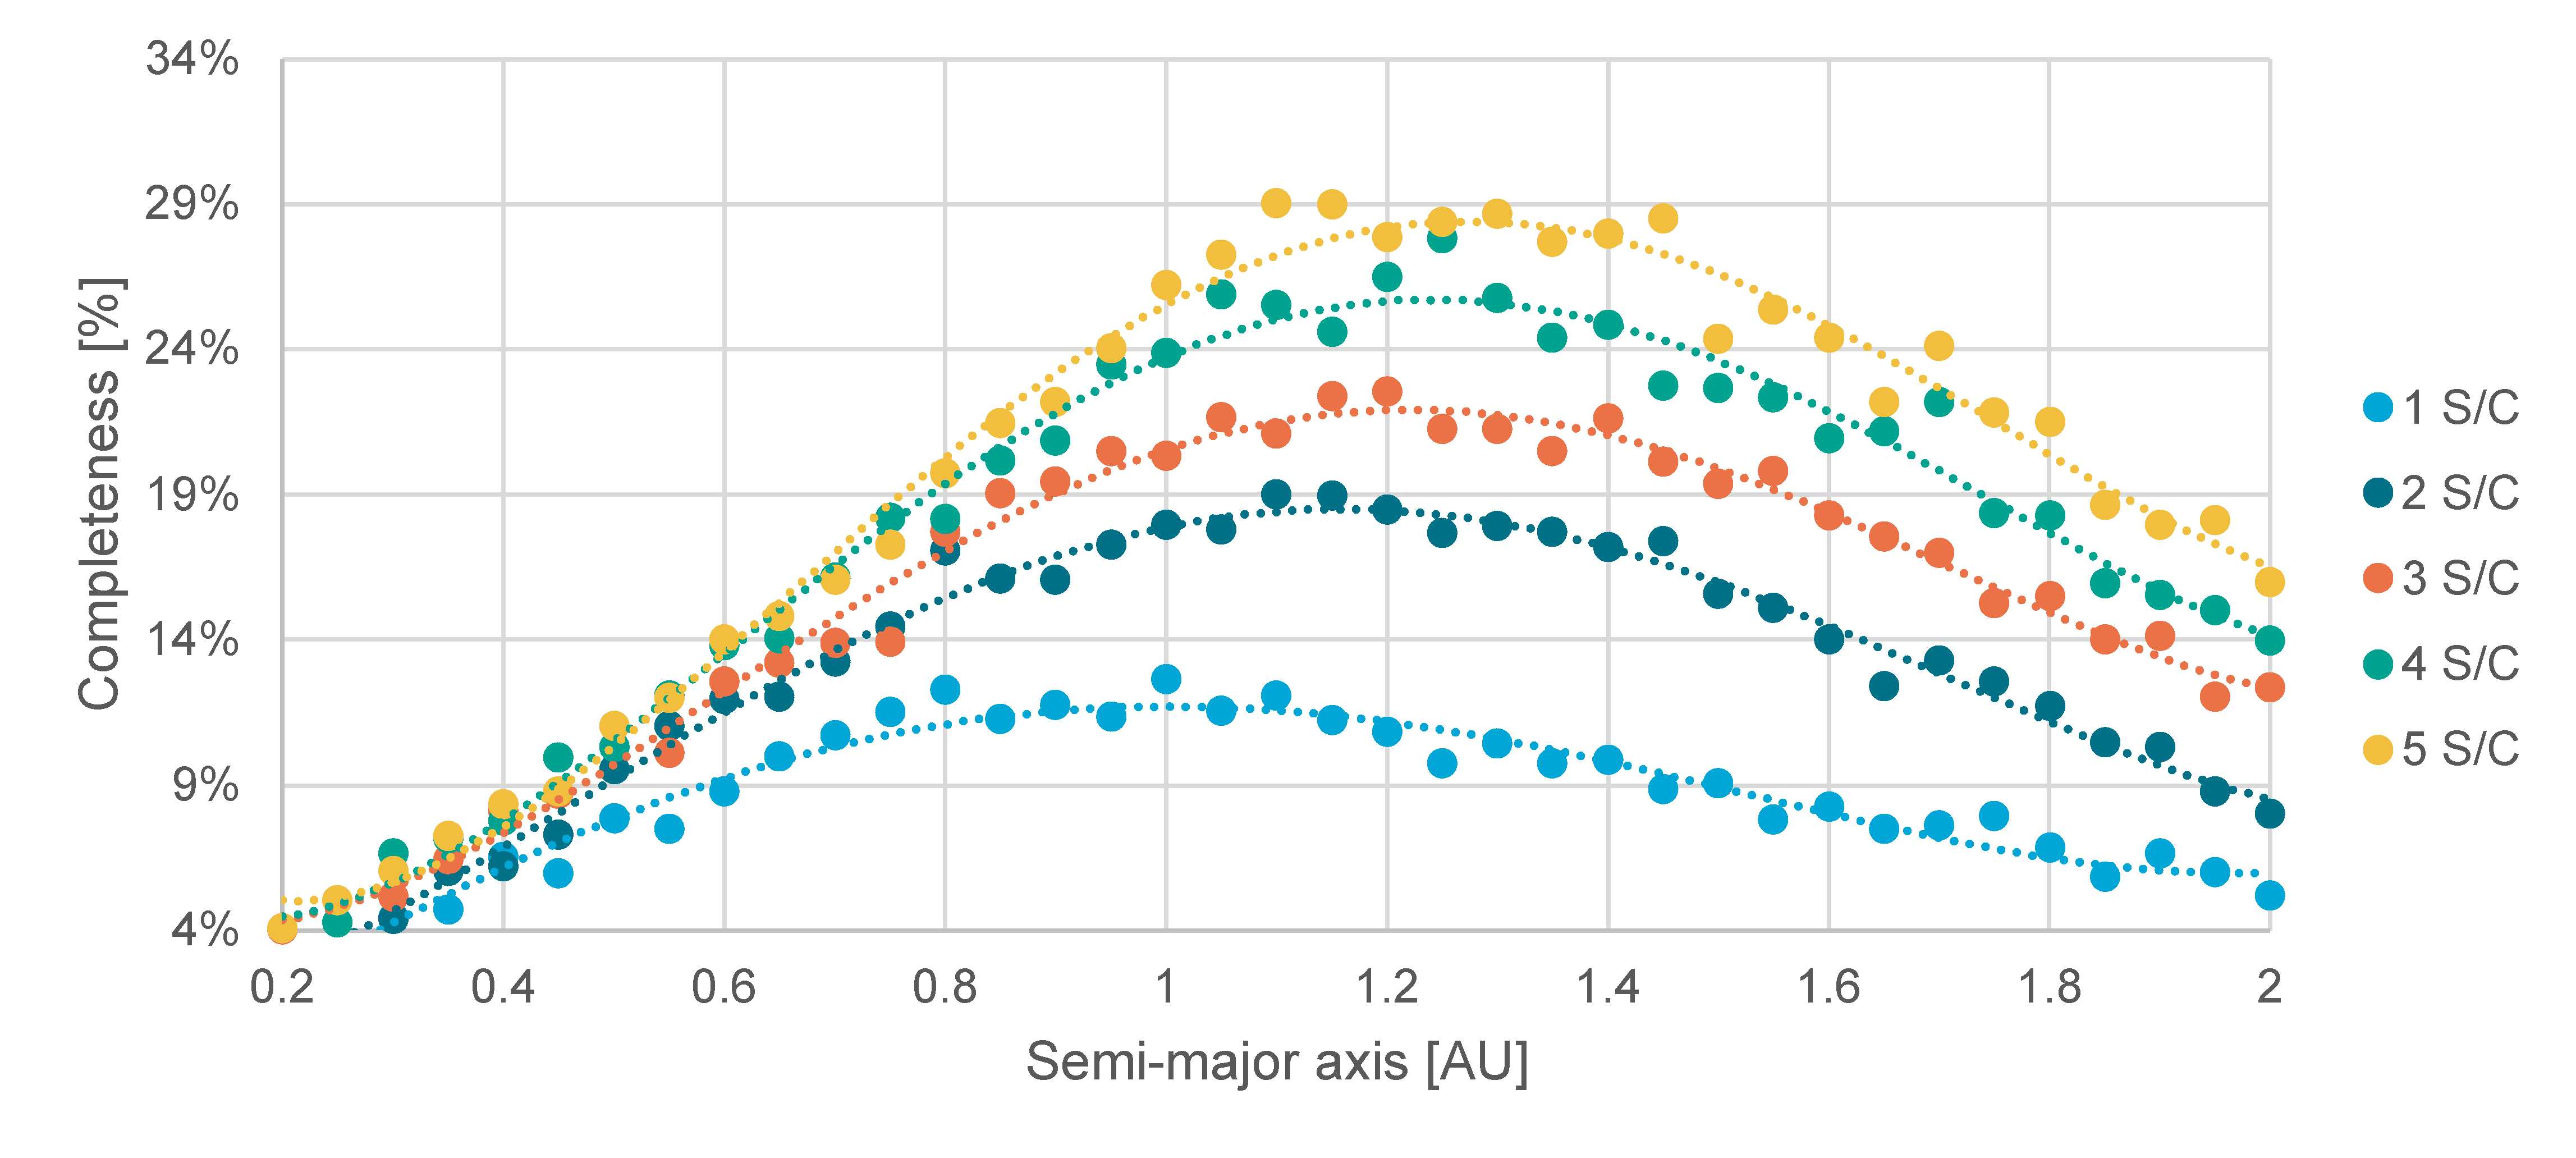
\includegraphics[width=0.8\textwidth]{img/vis_semi_maj.pdf}
 \caption{Visual light survey performance as a function of semi-major axis for 1 to 5 spacecraft. Corresponding eccentricity and angular separation of spacecraft are optimized using a grid search for each point.}
 \label{fig:vis_semi_maj}
\end{figure}

\begin{figure}[htbp]
 \centering
 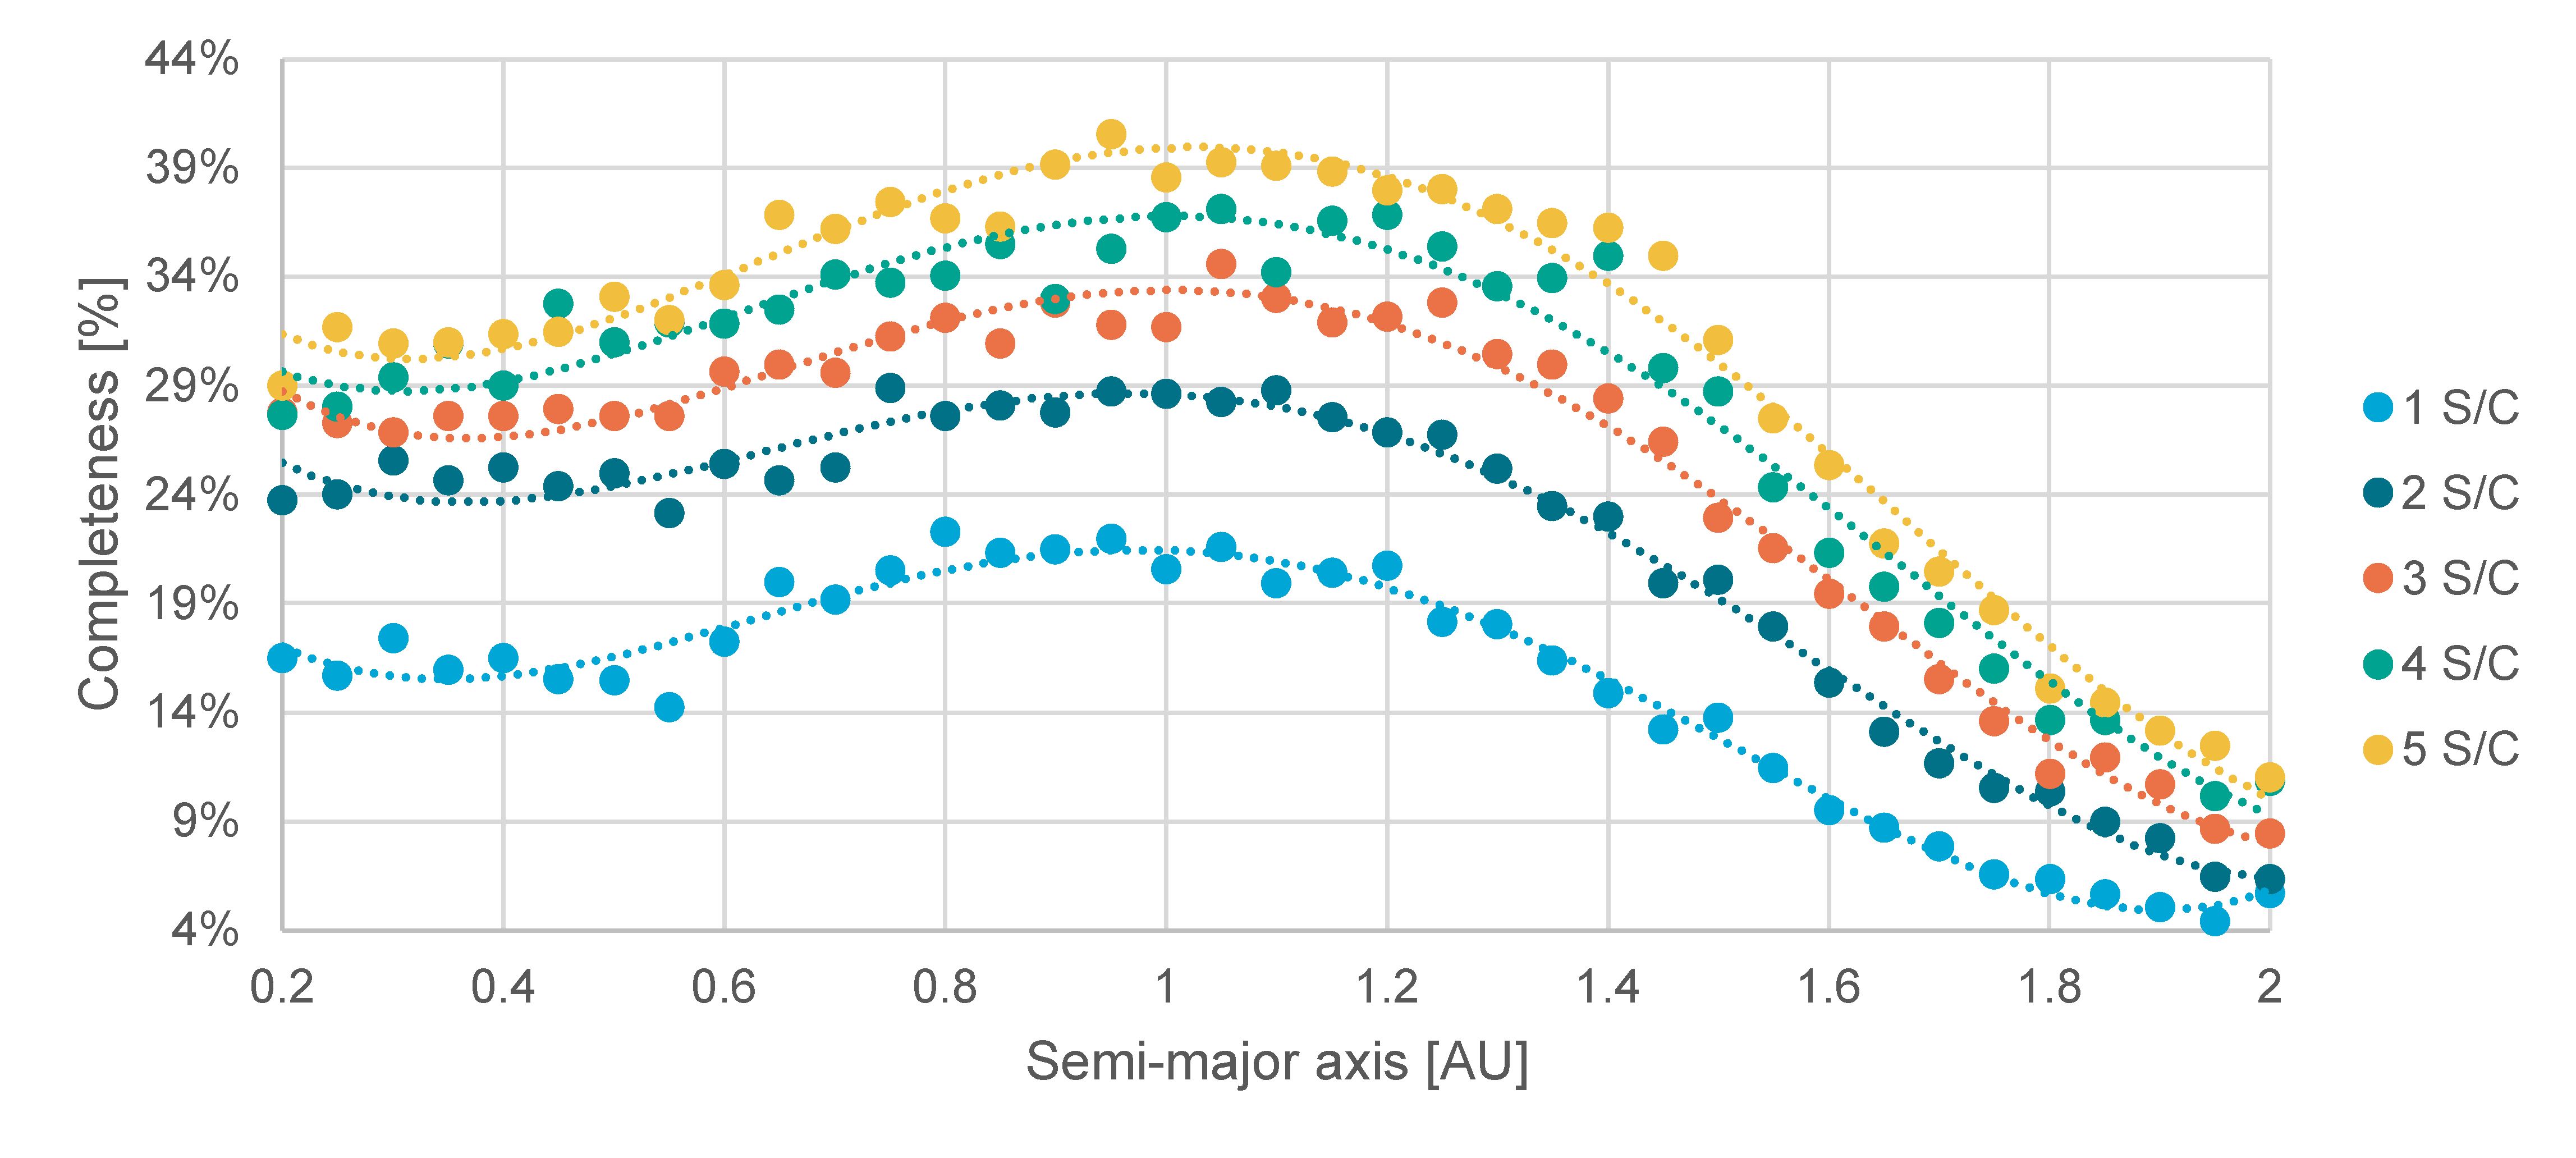
\includegraphics[width=0.8\textwidth]{img/tir_semi_maj.pdf}
 \caption{Thermal infrared survey performance as a function of semi-major axis for 1 to 5 spacecraft. Corresponding eccentricity and angular separation of spacecraft are optimized using a grid search for each point.}
 \label{fig:tir_semi_maj}
\end{figure}

In \autoref{fig:vis_semi_maj}, the expected survey performance as a function of semi-major axis is shown for visual light systems, and in \autoref{fig:tir_semi_maj} for thermal infrared systems. It can be clearly observed that the semi-major axis has an optimal value, which is dependent on the number of spacecraft. In addition, the region surrounding the optimum is very flat. Thus, locally, the solution is not sensitive to changes in semi-major axis up to a distance of approximately 0.1 AU from the optimum. There is however some variance present in the results due to the stochastic elements of the simulation. Two important conclusions are drawn here: Firstly, a wide range of semi-major axes lead to a well performing system. Secondly, due to the variance in results, it is difficult to pinpoint an exact optimal value. Therefore, in mission design, other considerations can and should be prioritized to determine a more precise semi-major axis. \\

The second factor of note is the change in the optimal semi-major axis as the number of spacecraft increases. It can be observed that increasing the number of spacecraft in the system leads to an increase in the optimal semi-major axis where the system should be positioned. This is further illustrated in \autoref{fig:semi_maj_function_of_n}, where the optimal semi-major axis is given as a function of the number of spacecraft explicitly. Here, it can also be seen that there is a large range of values possible for the semi-major axis. In addition, the semi-major axis becomes larger for higher numbers of spacecraft: E.g., a thermal infrared-equipped system comprising a single spacecraft should utilize a 0.9-1.0 AU orbit, but this increases to 1.0-1.1 for 3-5 spacecraft. Further increases in the number of spacecraft yield further increases. An explanation for this phenomenon is proposed in \autoref{sec:results_explanation}.

\begin{figure}[htbp]
 \centering
 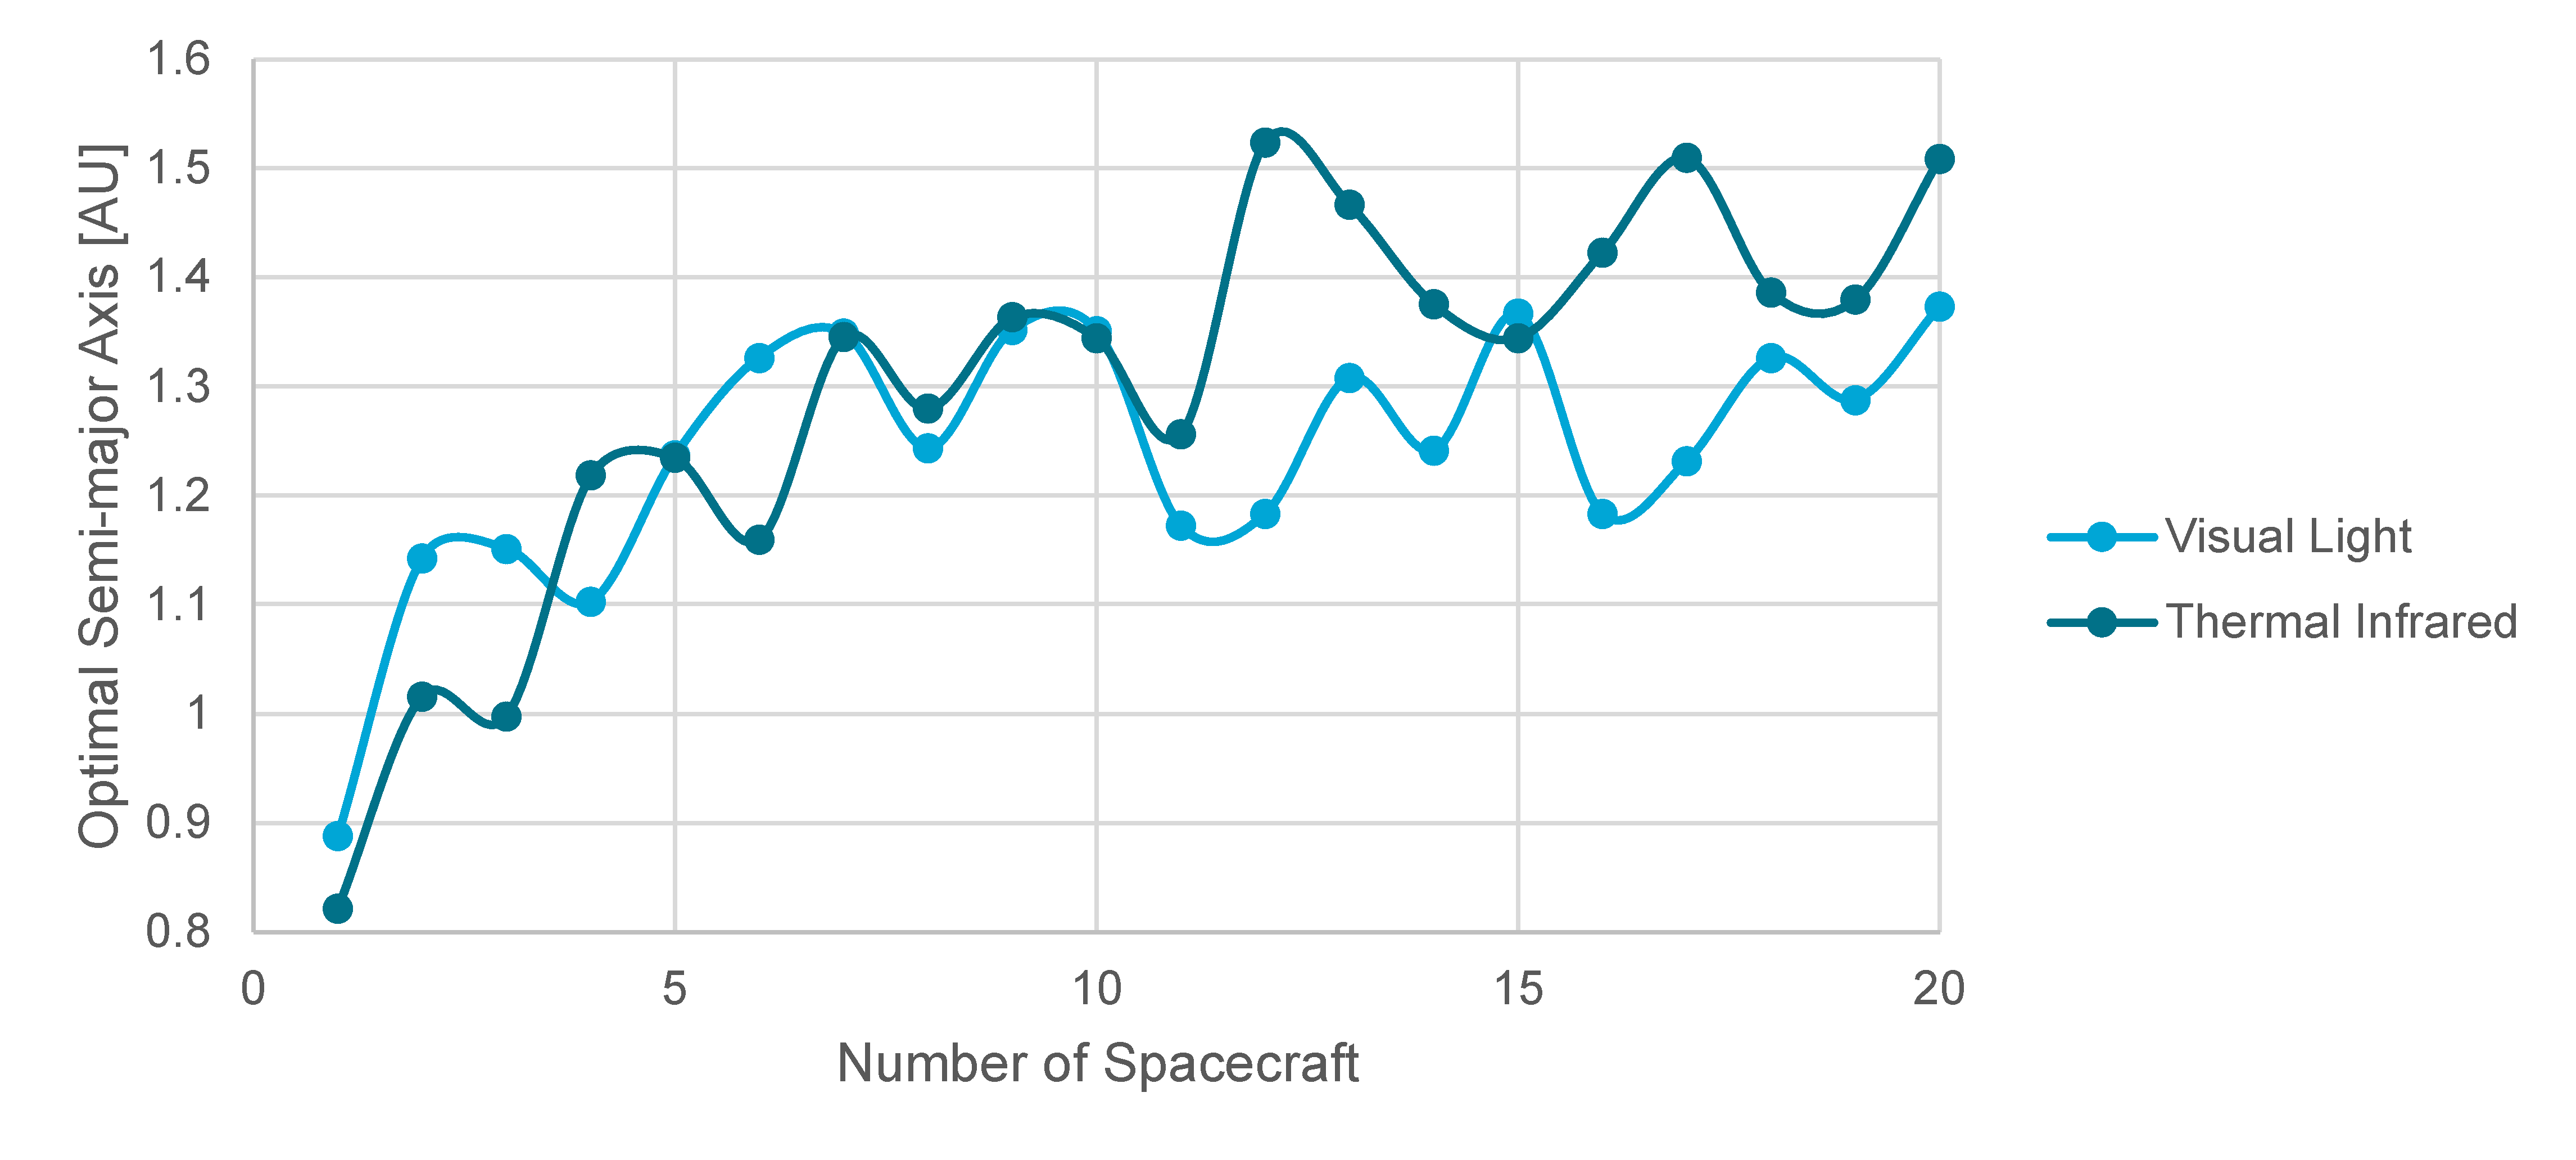
\includegraphics[width=0.8\textwidth]{img/semi_maj_function_of_n.pdf}
 \caption{Optimal semi-major axis as a function of the number of spacecraft in the system, including standard deviation bars. The eccentricity is zero, and the spacecraft are spread out equally. All values were optained using surrogate optimization, using 10 iterations to obtain the mean and standard deviation.}
 \label{fig:semi_maj_function_of_n}
\end{figure}



\subsection{Eccentricity}
\begin{figure}[htbp]
 \centering
 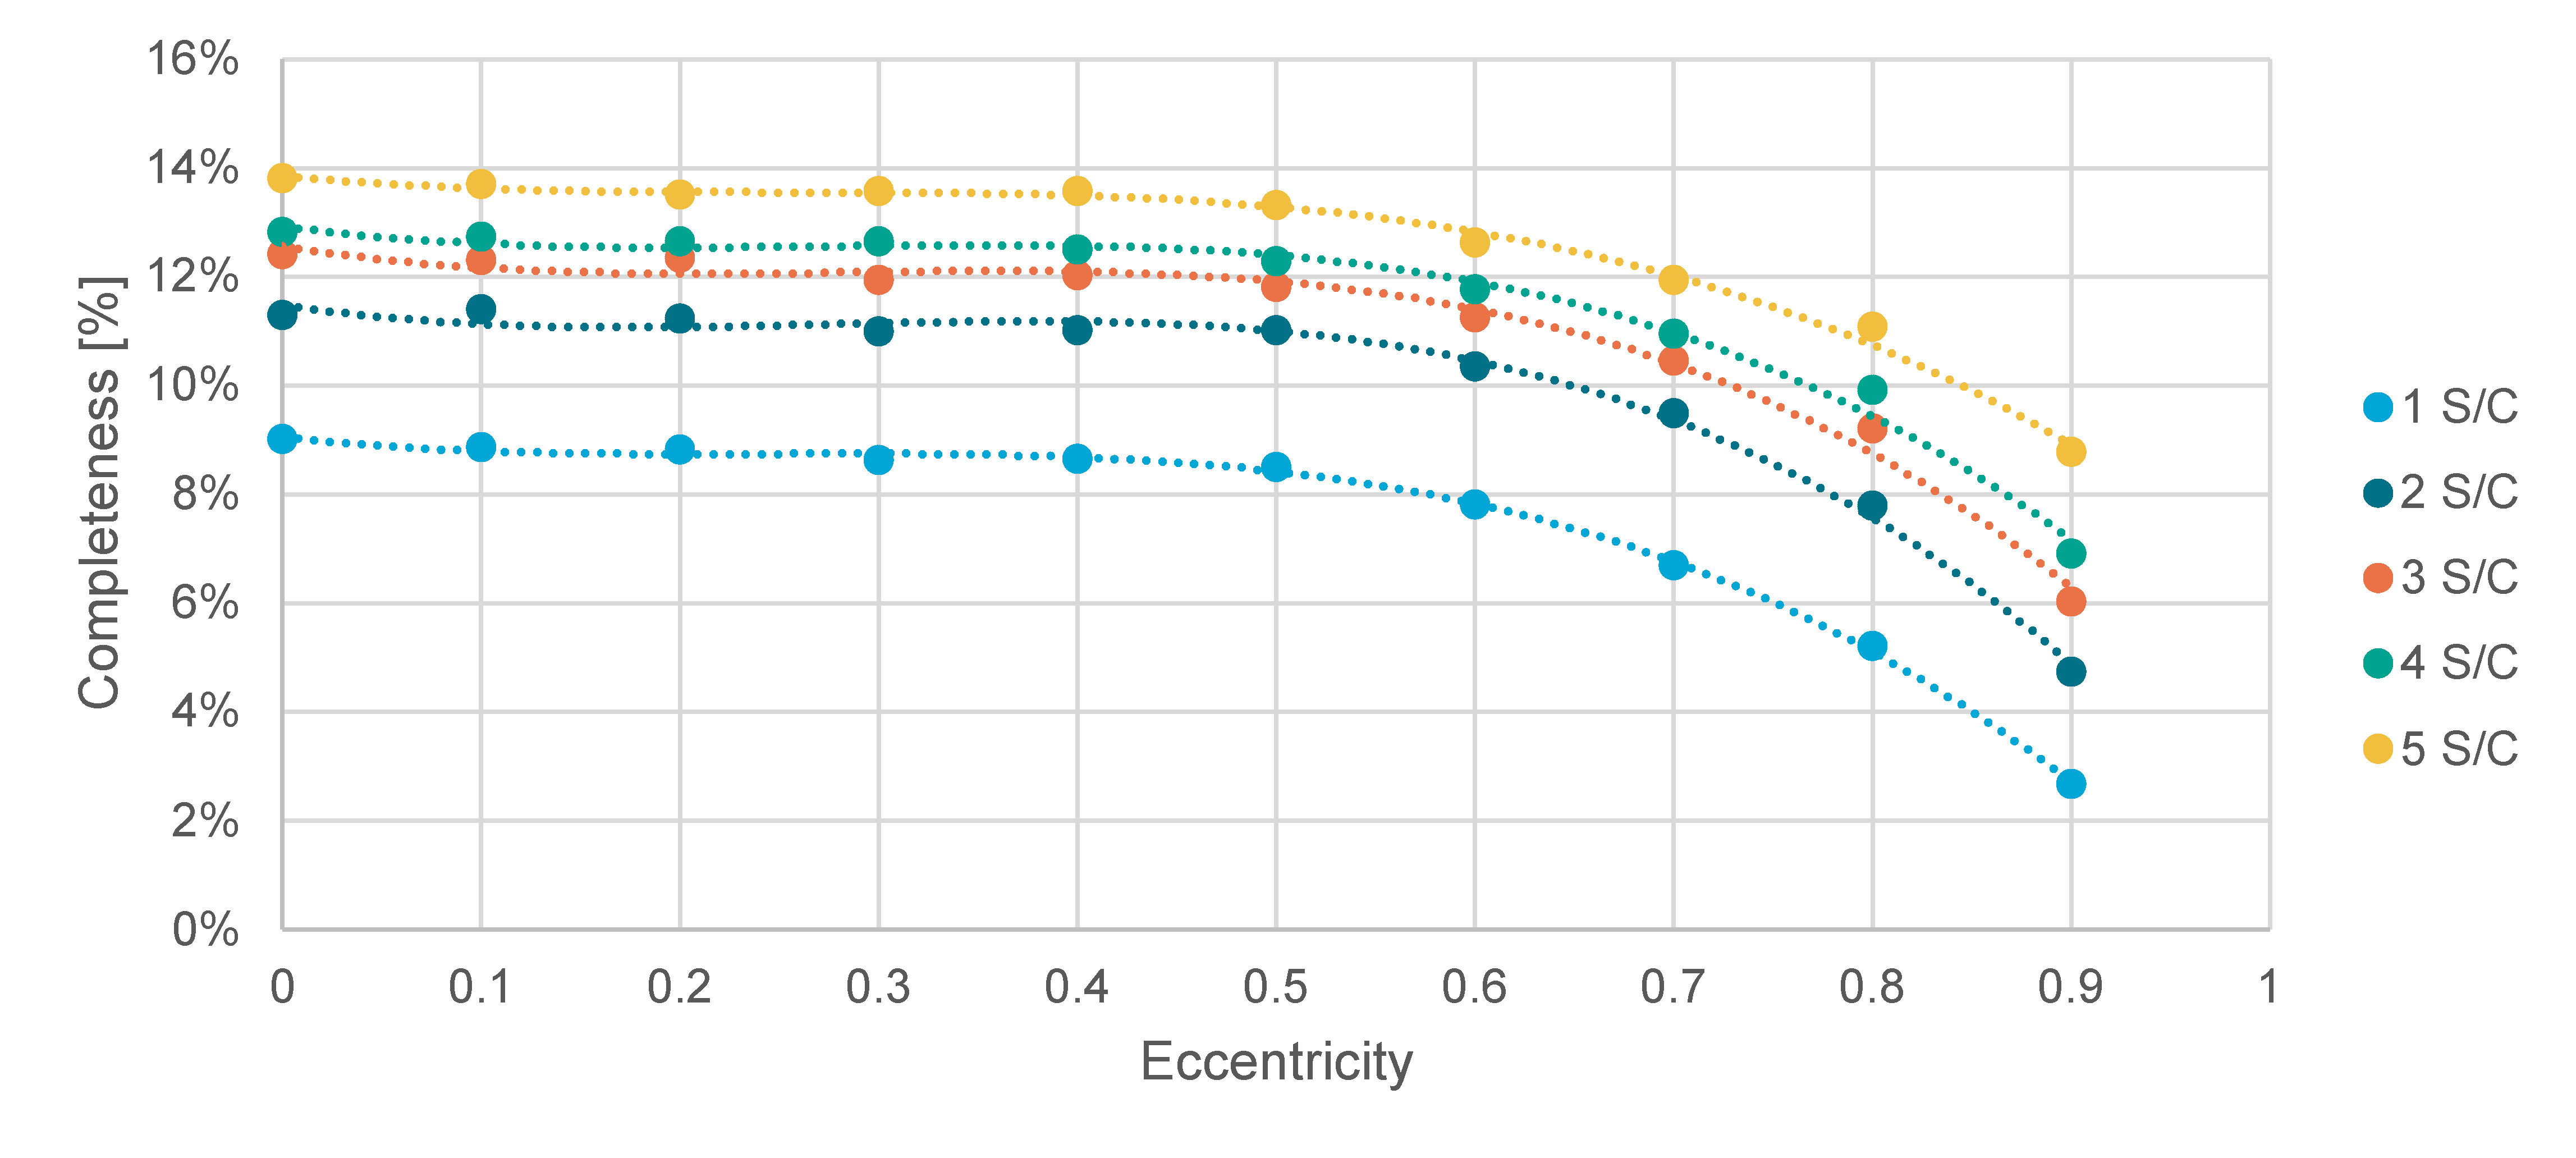
\includegraphics[width=0.8\textwidth]{img/vis_ecc.pdf}
 \caption{Visual light survey performance as a function of eccentricity for 1 to 5 spacecraft. Corresponding semi-major axis and angular separation of spacecraft are optimized using a grid search for each point.}
 \label{fig:vis_ecc}
\end{figure}

\begin{figure}[htbp]
 \centering
 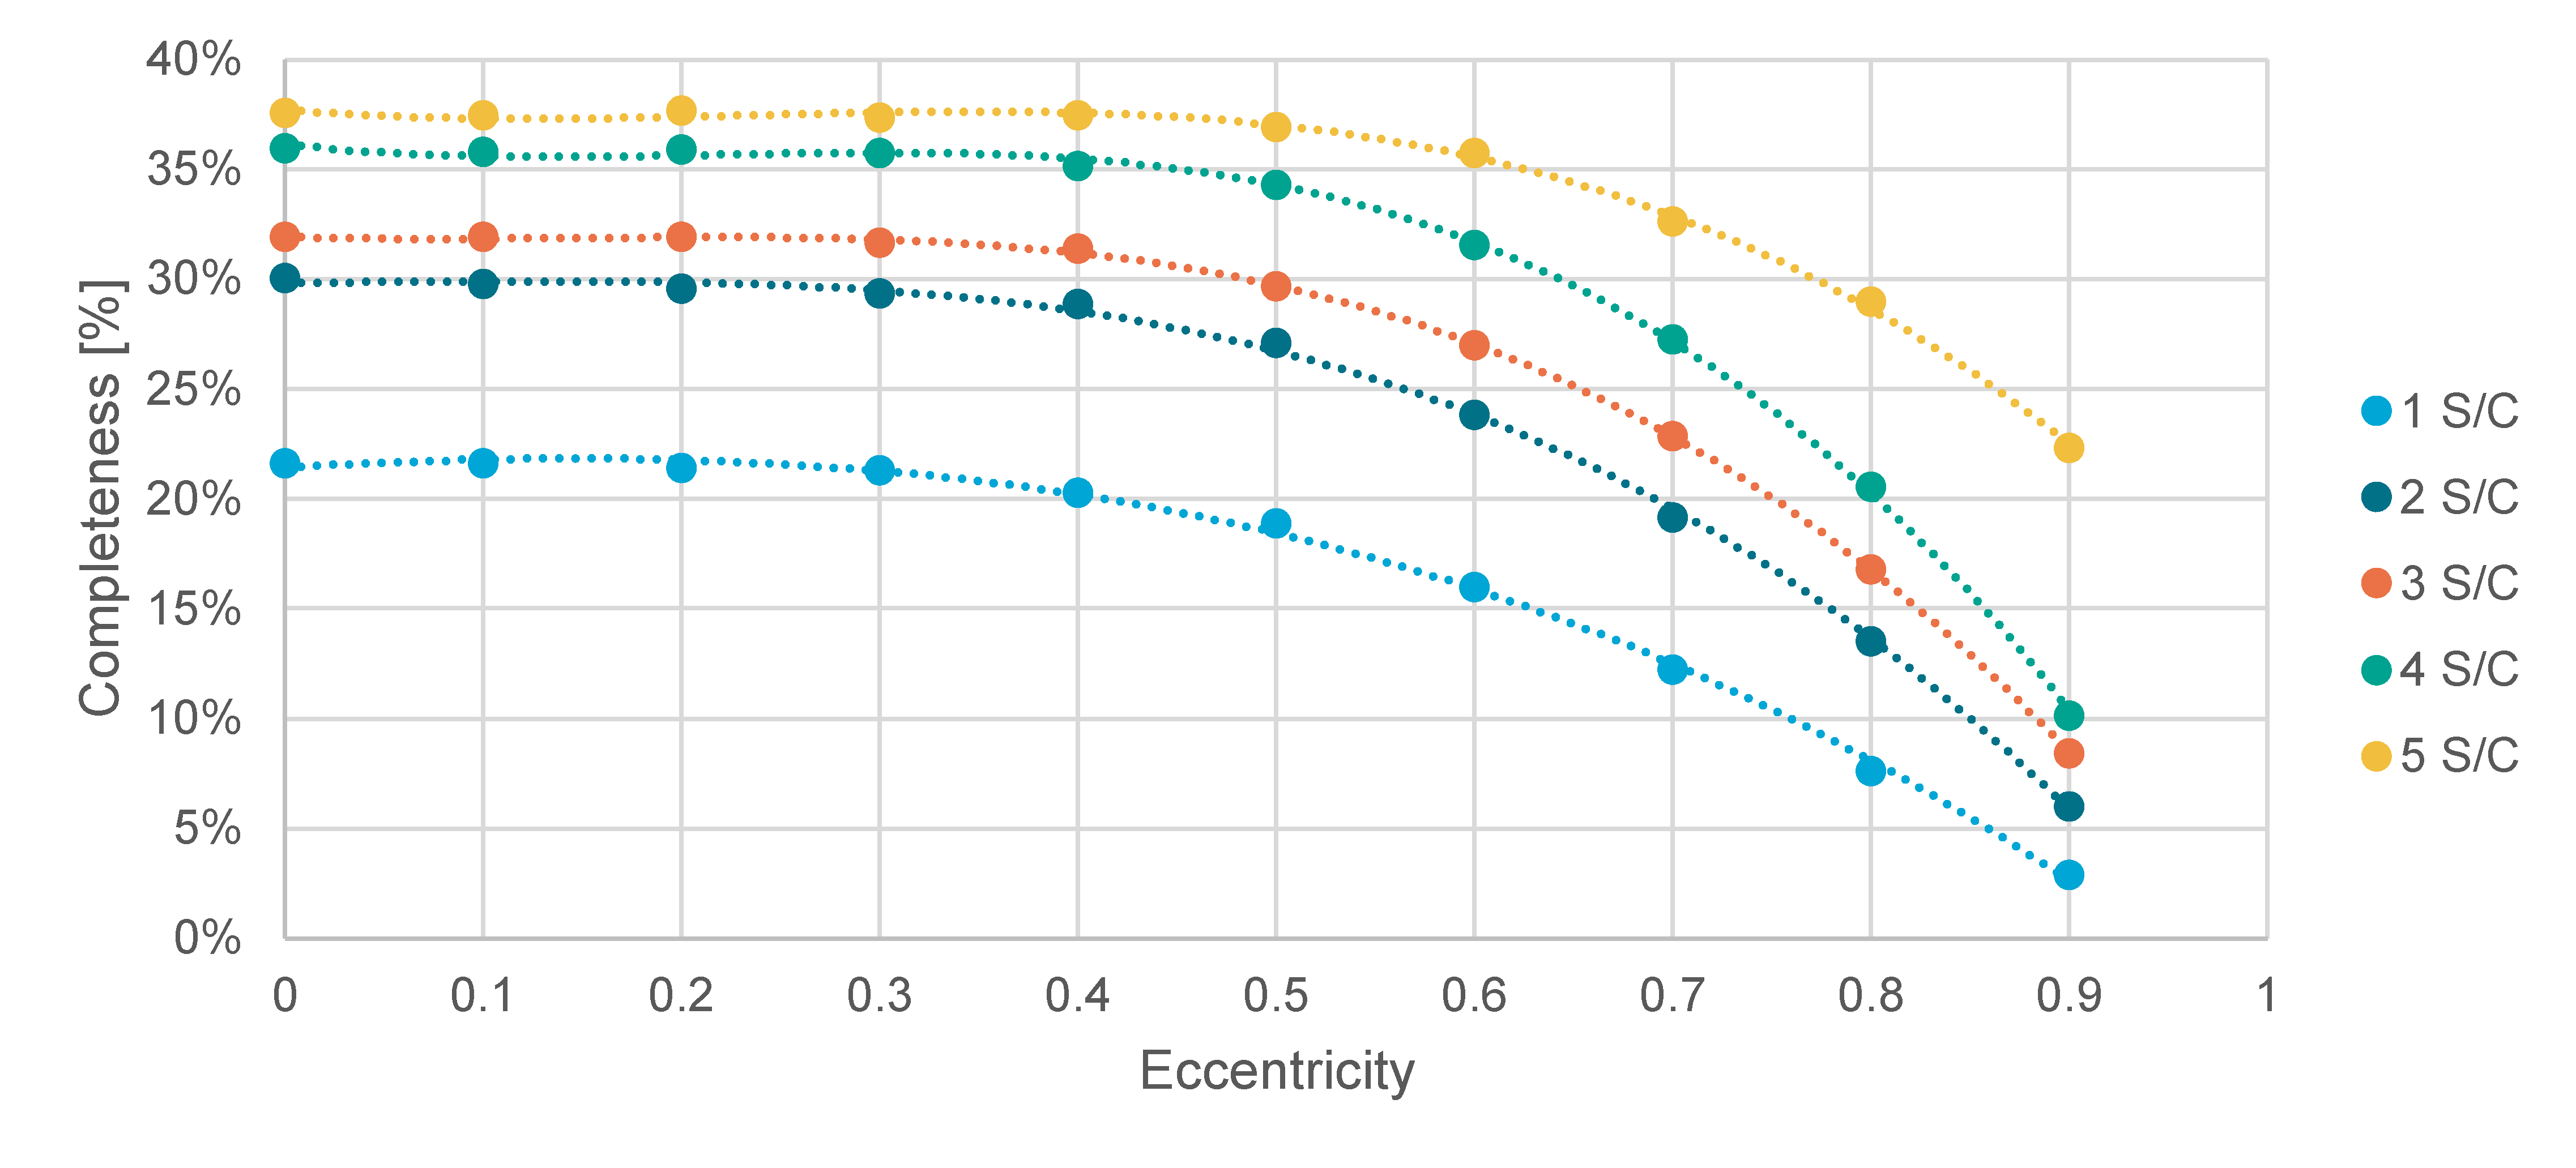
\includegraphics[width=0.8\textwidth]{img/tir_ecc.pdf}
 \caption{Thermal infrared survey performance as a function of eccentricity for 1 to 5 spacecraft. Corresponding semi-major axis and angular separation of spacecraft are optimized using a grid search for each point.}
 \label{fig:tir_ecc}
\end{figure}

Results with regards to varying the eccentricity are shown in \autoref{fig:vis_ecc} for visual light systems and \autoref{fig:tir_ecc} for thermal infrared systems. It is readily apparent that for both systems, a circular orbit is preferred. It is hypothesized that this is the case because eccentricity causes the system to deviate from the optimal semi-major axis found in the previous subsection. This is further supported by the empirical finding that the optimal semi-major axis at a given eccentricity results in an apohelion distance roughly equal to the optimal semi-major axis at 0 eccentricity. That is:
\begin{equation}
 a_{opt}(e) \approx \frac{a_{opt}(0)}{1+e}
\end{equation}
This is further illustrated in \autoref{fig:eccentricity_optimal}. This result is theorized to occur because the spacecraft will, in this solution, still spend a large portion of its orbit in the optimal semi-major axis range. However, not enough data are available to establish statistical significance for this finding.

\begin{figure}[htbp]
 \centering
 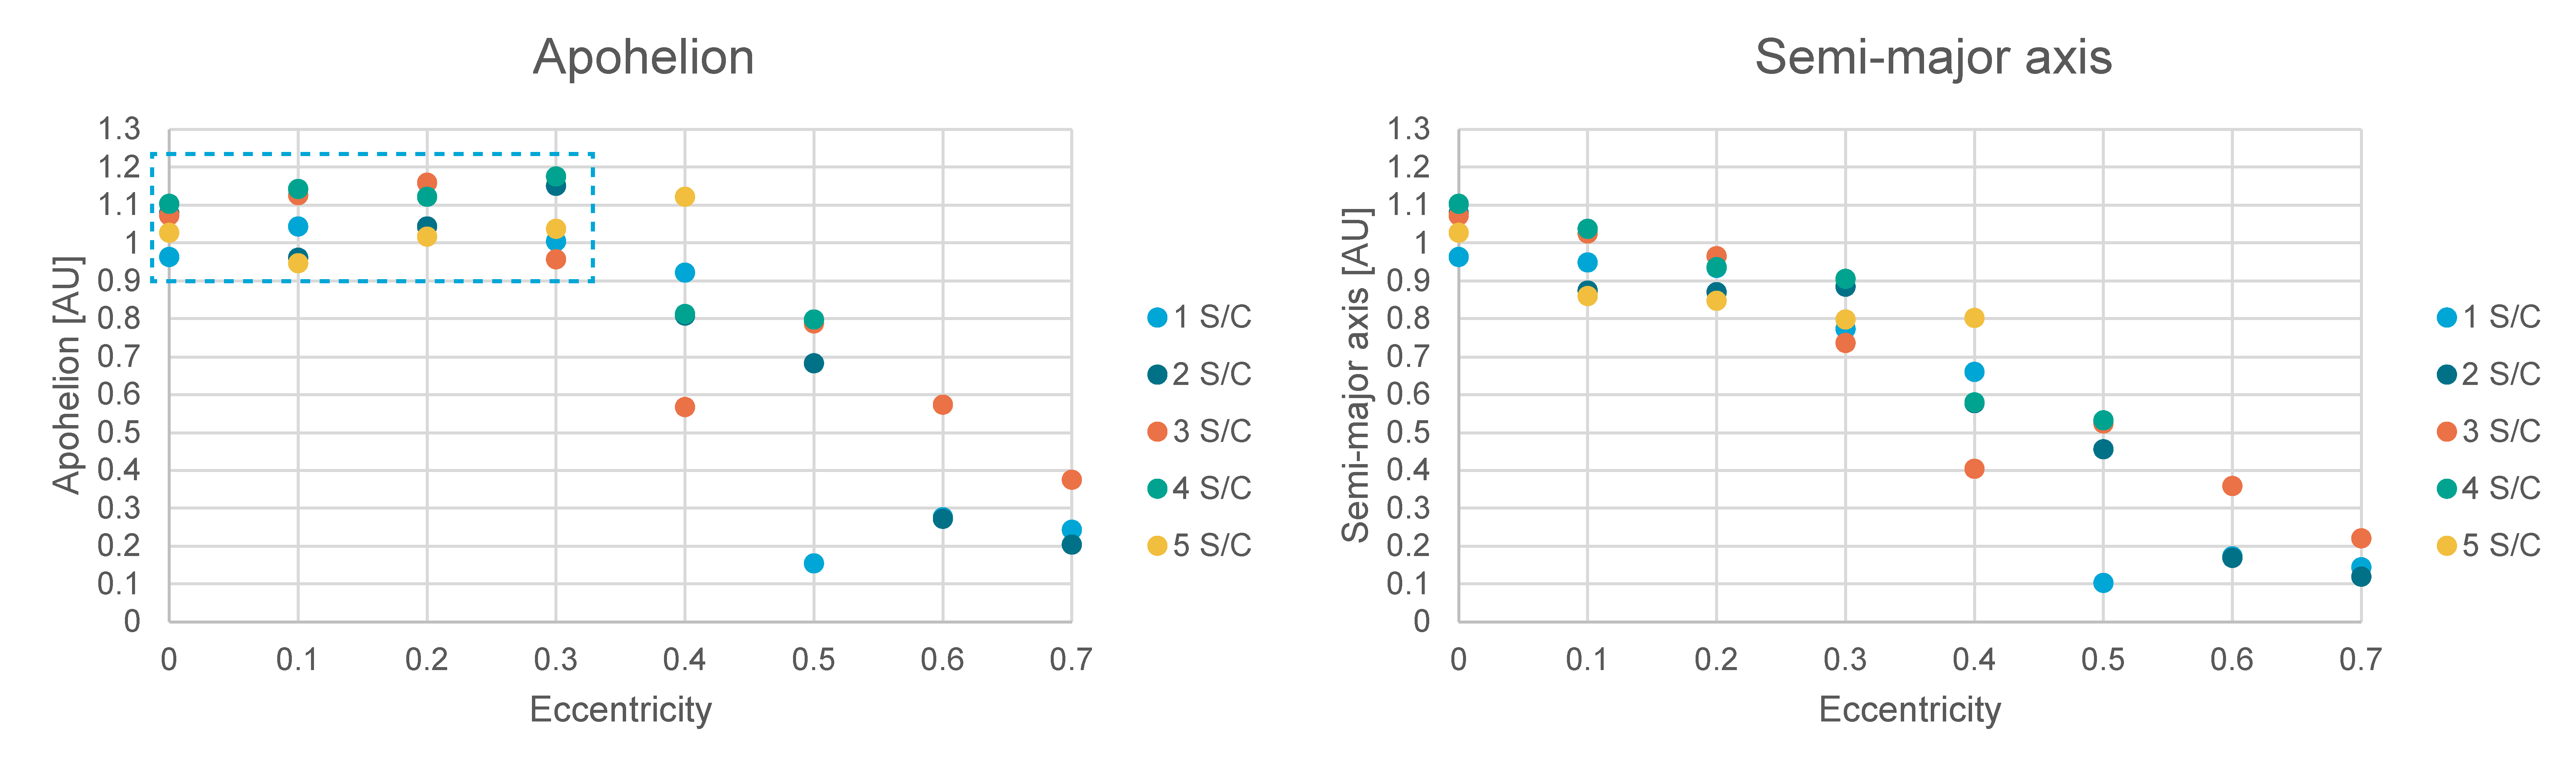
\includegraphics[width=1.0\textwidth]{img/eccentricity_optimal.pdf}
 \caption{Relationship between optimal semi-major axis, eccentricity, and the resulting apohelion for 1-5 spacecraft. It can be seen that the system attempts to maintain the same apohelion for low eccentricities. Corresponding semi-major axis and angular separation of spacecraft are optimized using a grid search for each point.}
 \label{fig:eccentricity_optimal}
\end{figure}


\subsection{Mean Anomaly at Epoch}
\begin{figure}
 \centering
 \includegraphics[width=1.0\textwidth]{img/spread_illustration.png}
 \caption{Illustration of a high ($2\pi/5~\mathrm{rad}$) and a low ($0.3~\mathrm{rad}$) inter-spacecraft distance.}
 \label{fig:spread_illustration}
\end{figure}

The last parameter to be considered for the co-orbital solutions is the mean anomaly at epoch. As previously explained, the mean anomaly will not be considered for each spacecraft separately. Instead, the concept of inter-spacecraft spread is introduced. This inter-spacecraft spread is simply defined as the difference in anomaly at epoch of one spacecraft to the next, in such a way that the formation is centered around $\theta=0$. This means that, with inter-spacecraft spread $\Delta \theta$, the mean anomaly at epoch $\theta$ of spacecraft $n$ in a system of $N$ spacecraft is:
\begin{equation}
 \theta_n = (n-1) \cdot \Delta \theta - \frac{N-1}{2}\Delta \theta
\end{equation}
This equation and the resulting formation is shown in \autoref{fig:spread_illustration}. A lower boundary of 0.3 rad ($\approx 17.2^\circ$) was chosen to ensure triangulation would remain possible. In addition, to maintain the separation between all spacecraft, the full formation can not span more than $2\pi$ rad. This results in the boundaries $0.3 \leq \Delta \theta \leq 2\pi/N$. The hypothesized effect of changing the spread is composed of two effects: On the one hand, spreading out the spacecraft more allows for viewing a larger portion of the sky simultaneously, and reduces blind spots, as explained in \autoref{sec:researchmultispacecraft}. On the other hand, as spacecraft are closer together, the chances of obtaining a simultaneous detection of the same asteroid - and thereby achieving triangulation - is increased, thereby leading to a faster detection.\\

\begin{figure}[htbp]
 \centering
 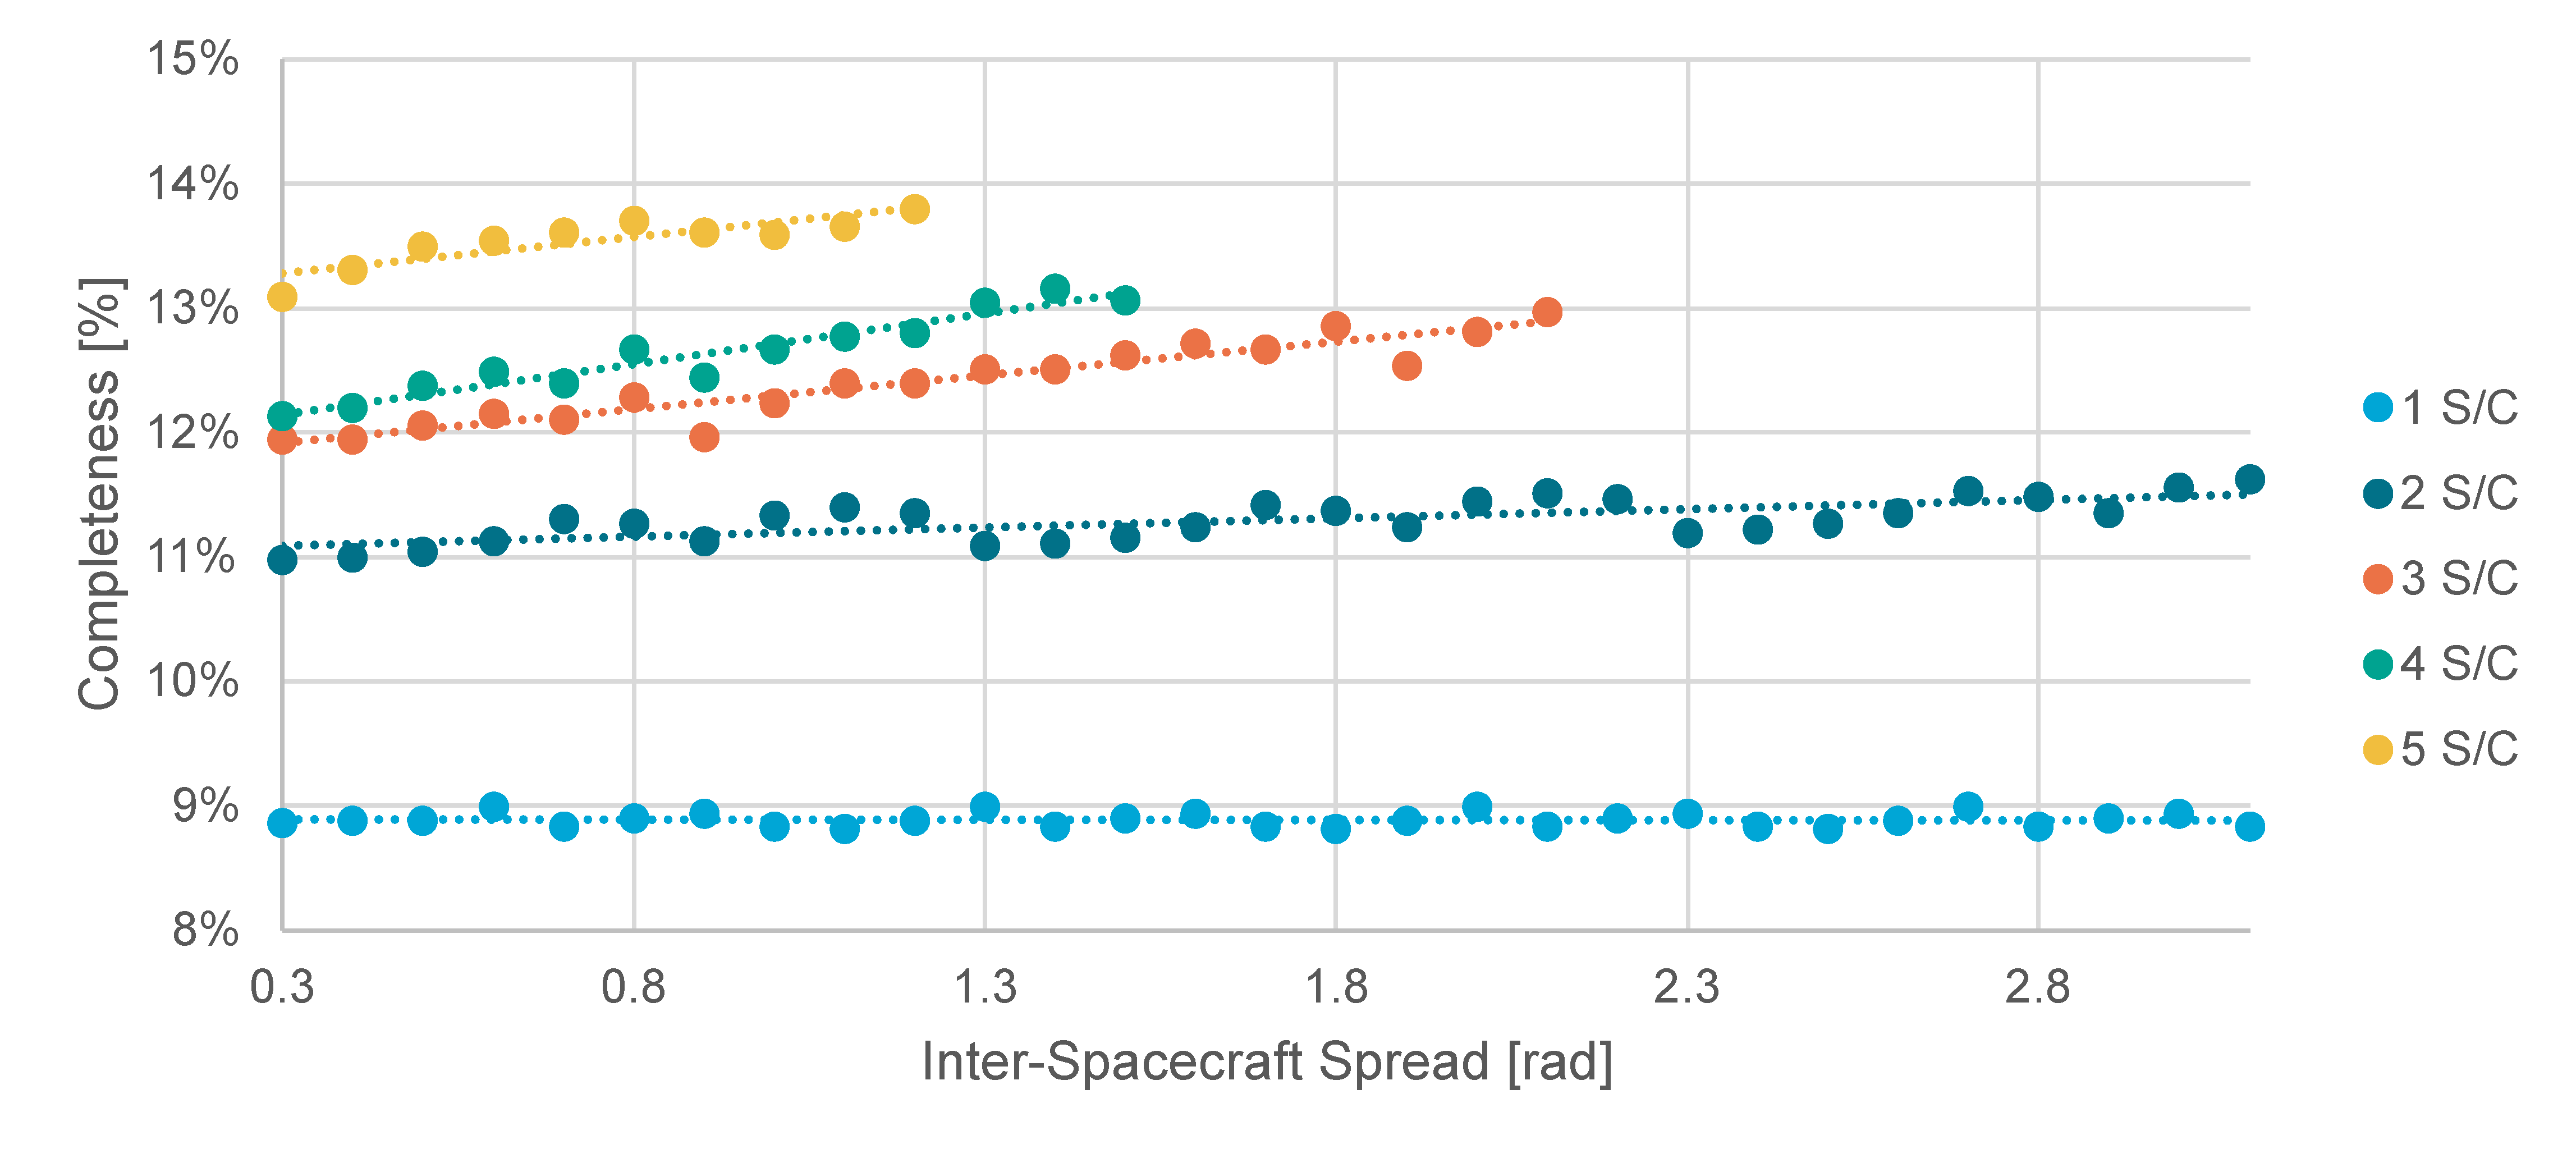
\includegraphics[width=0.8\textwidth]{img/vis_spread.pdf}
 \caption{Visual light survey performance as a function of angular separation between spacecraft for 1 to 5 spacecraft. Corresponding semi-major axis and eccentricity are optimized using a grid search for each point.}
 \label{fig:vis_spread}
\end{figure}

\begin{figure}[htbp]
 \centering
 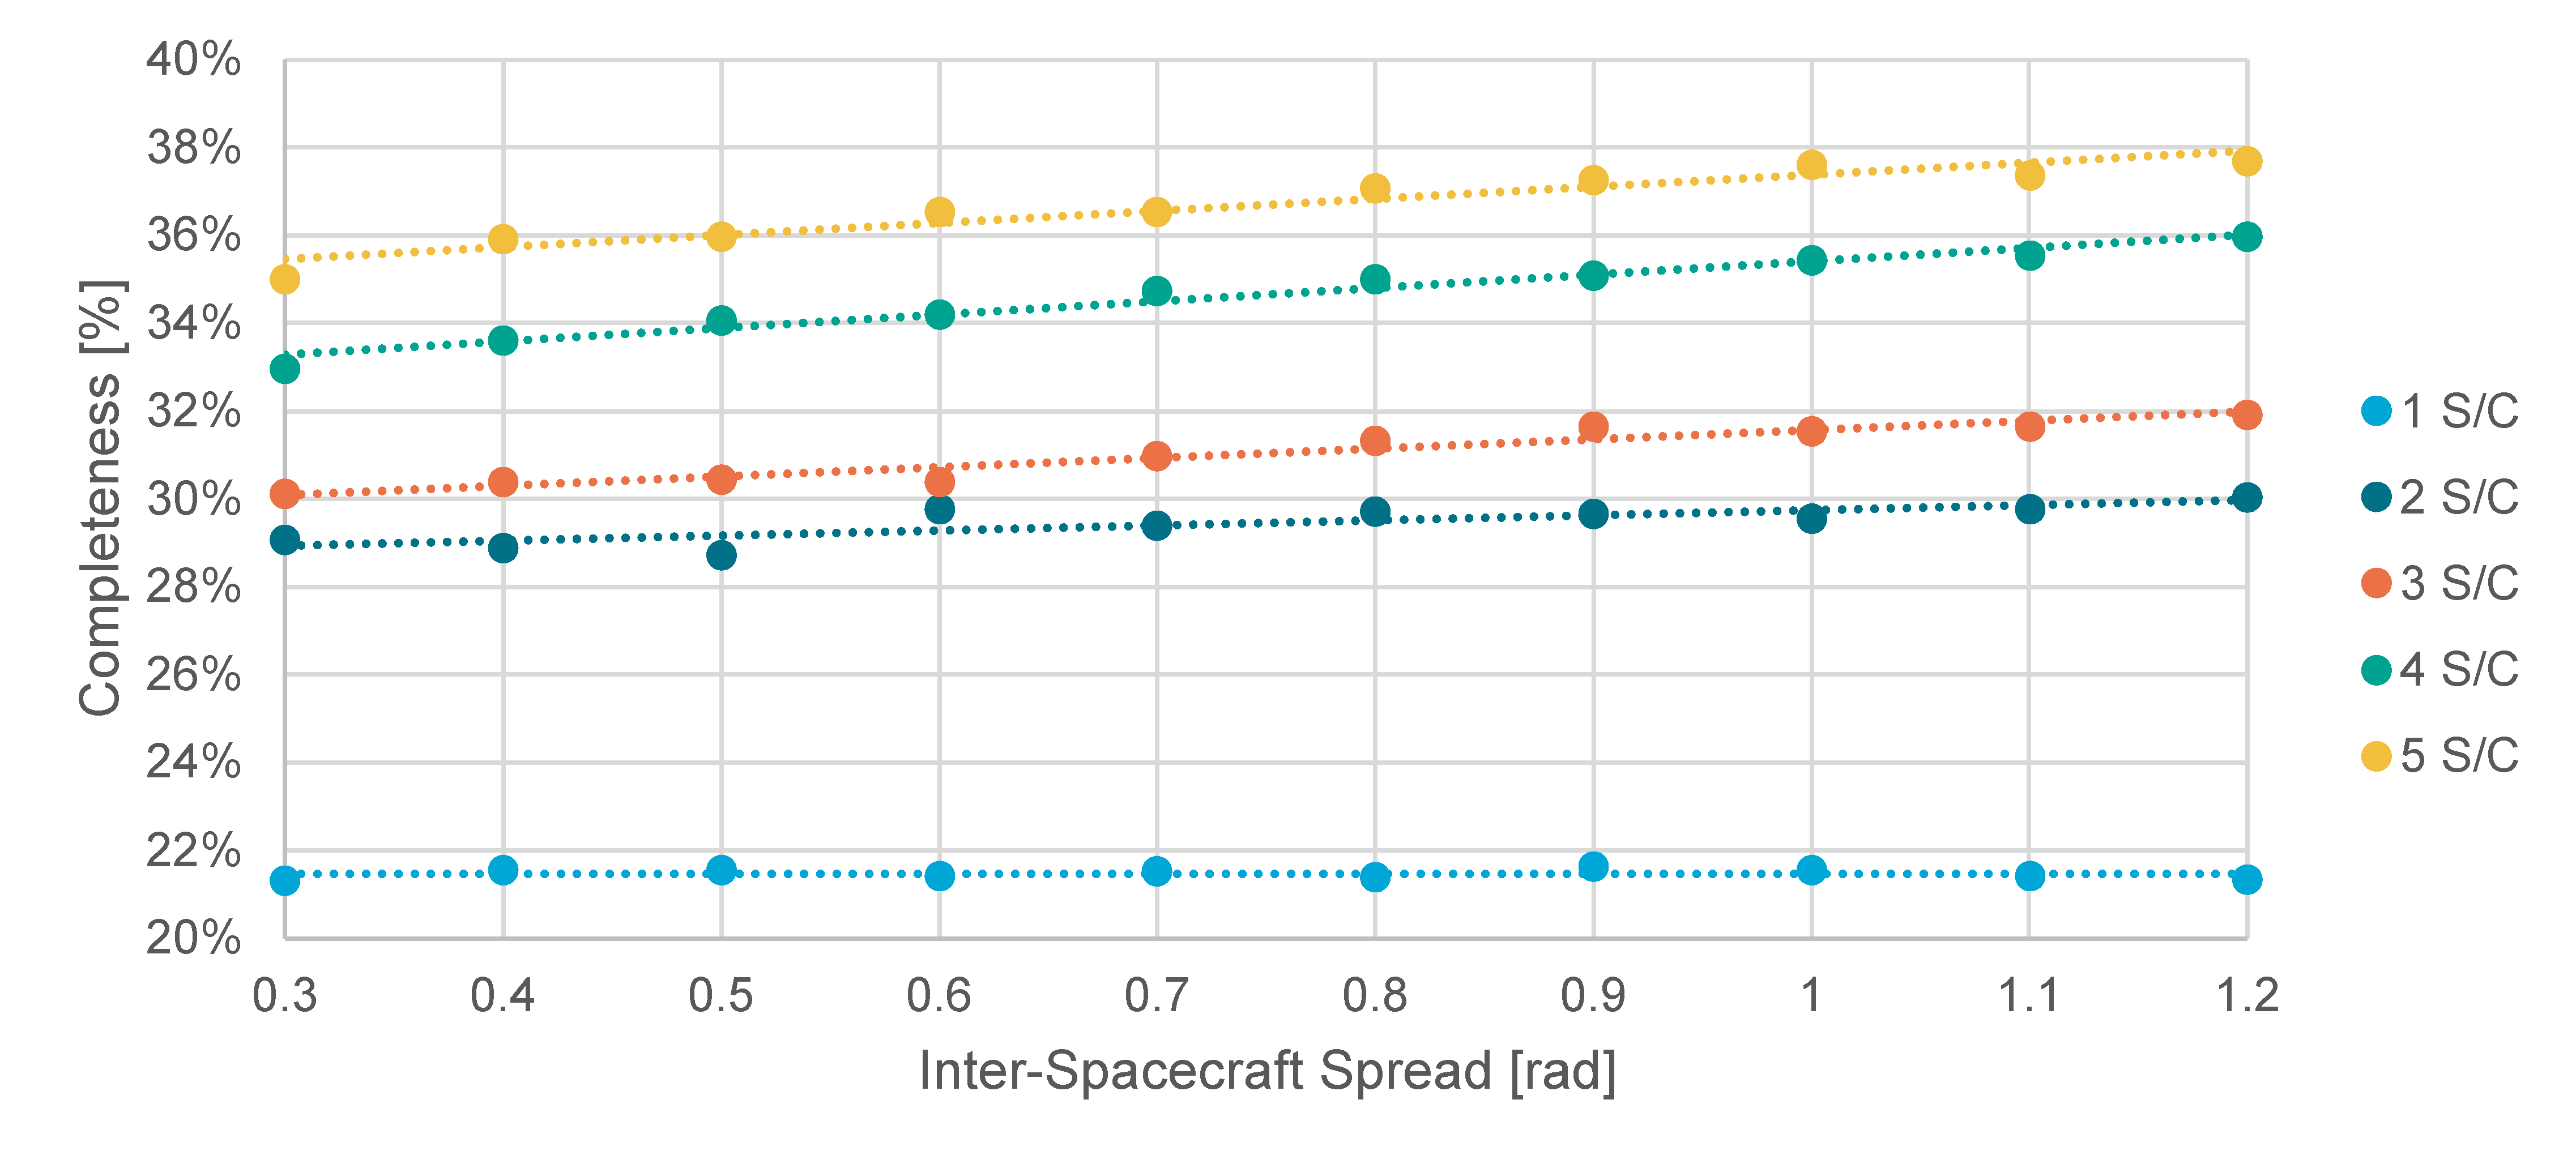
\includegraphics[width=0.8\textwidth]{img/tir_spread.pdf}
 \caption{Thermal infrared survey performance as a function of angular separation between spacecraft for 1 to 5 spacecraft. Corresponding semi-major axis and eccentricity are optimized using a grid search for each point.}
 \label{fig:tir_spread}
\end{figure}

Results for visual light and thermal infrared are shown in \autoref{fig:vis_spread} and \autoref{fig:tir_spread}, respectively. It is observed that an increase in the angular distance between the spacecraft will increase the performance of the system. Therefore, the effect of observing a larger part of the sky effectively is stronger than the increased chance at succesful triangulation. Practically, this implies that a multi-spacecraft survey should aim to distribute the spacecraft as much as possible over the orbit, even if e.g. communications requirements do not allow the system to be spread out over the entire orbit. In the next section, a hypothesis will be developed to explain the observed phenomena, and provide a basis for the prediction of the performance of the non-co-orbital systems to be considered later.

\section{Number of Spacecraft}
\label{sec:results_number}

\begin{figure}[htbp]
 \centering
 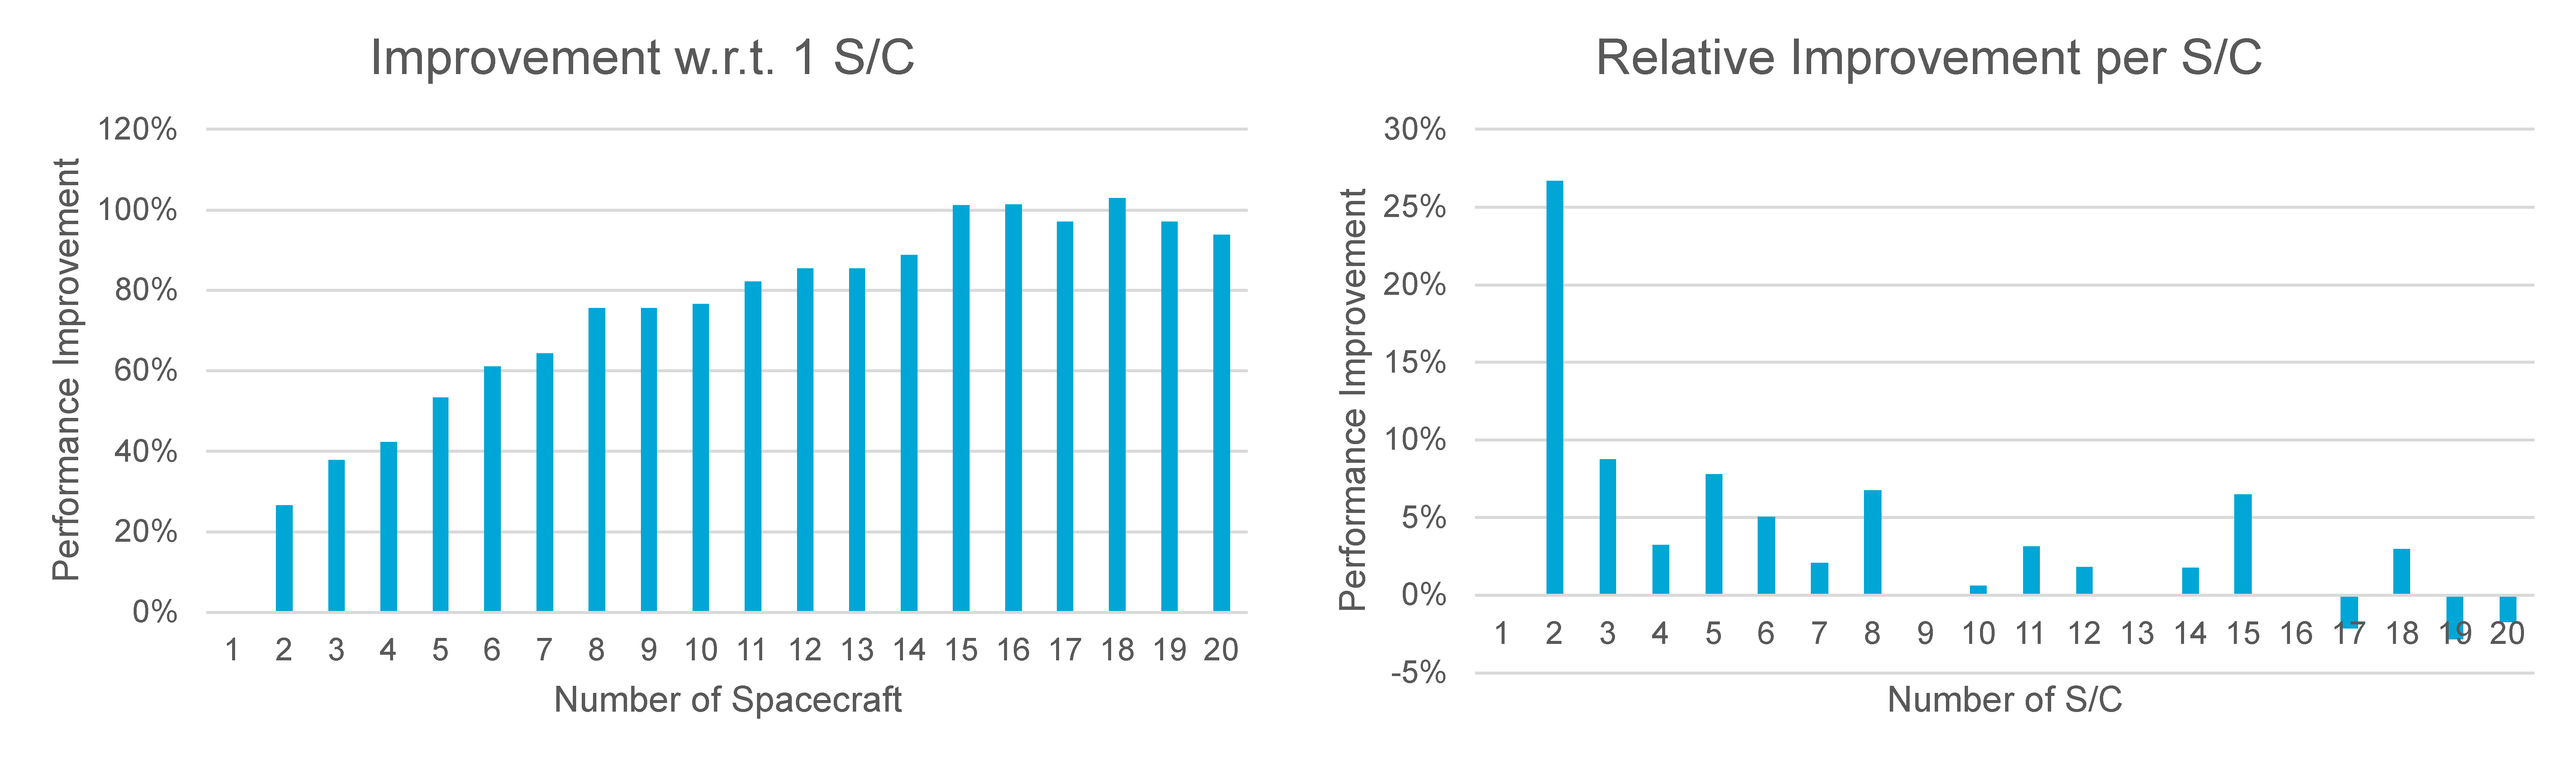
\includegraphics[width=1.0\textwidth]{img/number_sc_vis.pdf}
 \caption{Improvement in survey completeness gained by increasing the number of spacecraft in a purely visual light wavelength system, including standard deviation bars (from 10 iterations). The left graph shows the improvement of an $n$-spacecraft system with respect to a system of a single spacecraft, the right graph shows the improvement of an $n$-spacecraft system with respect to an $n-1$-spacecraft system.}
 \label{fig:results_number_vis}
\end{figure}


\begin{figure}[htbp]
 \centering
 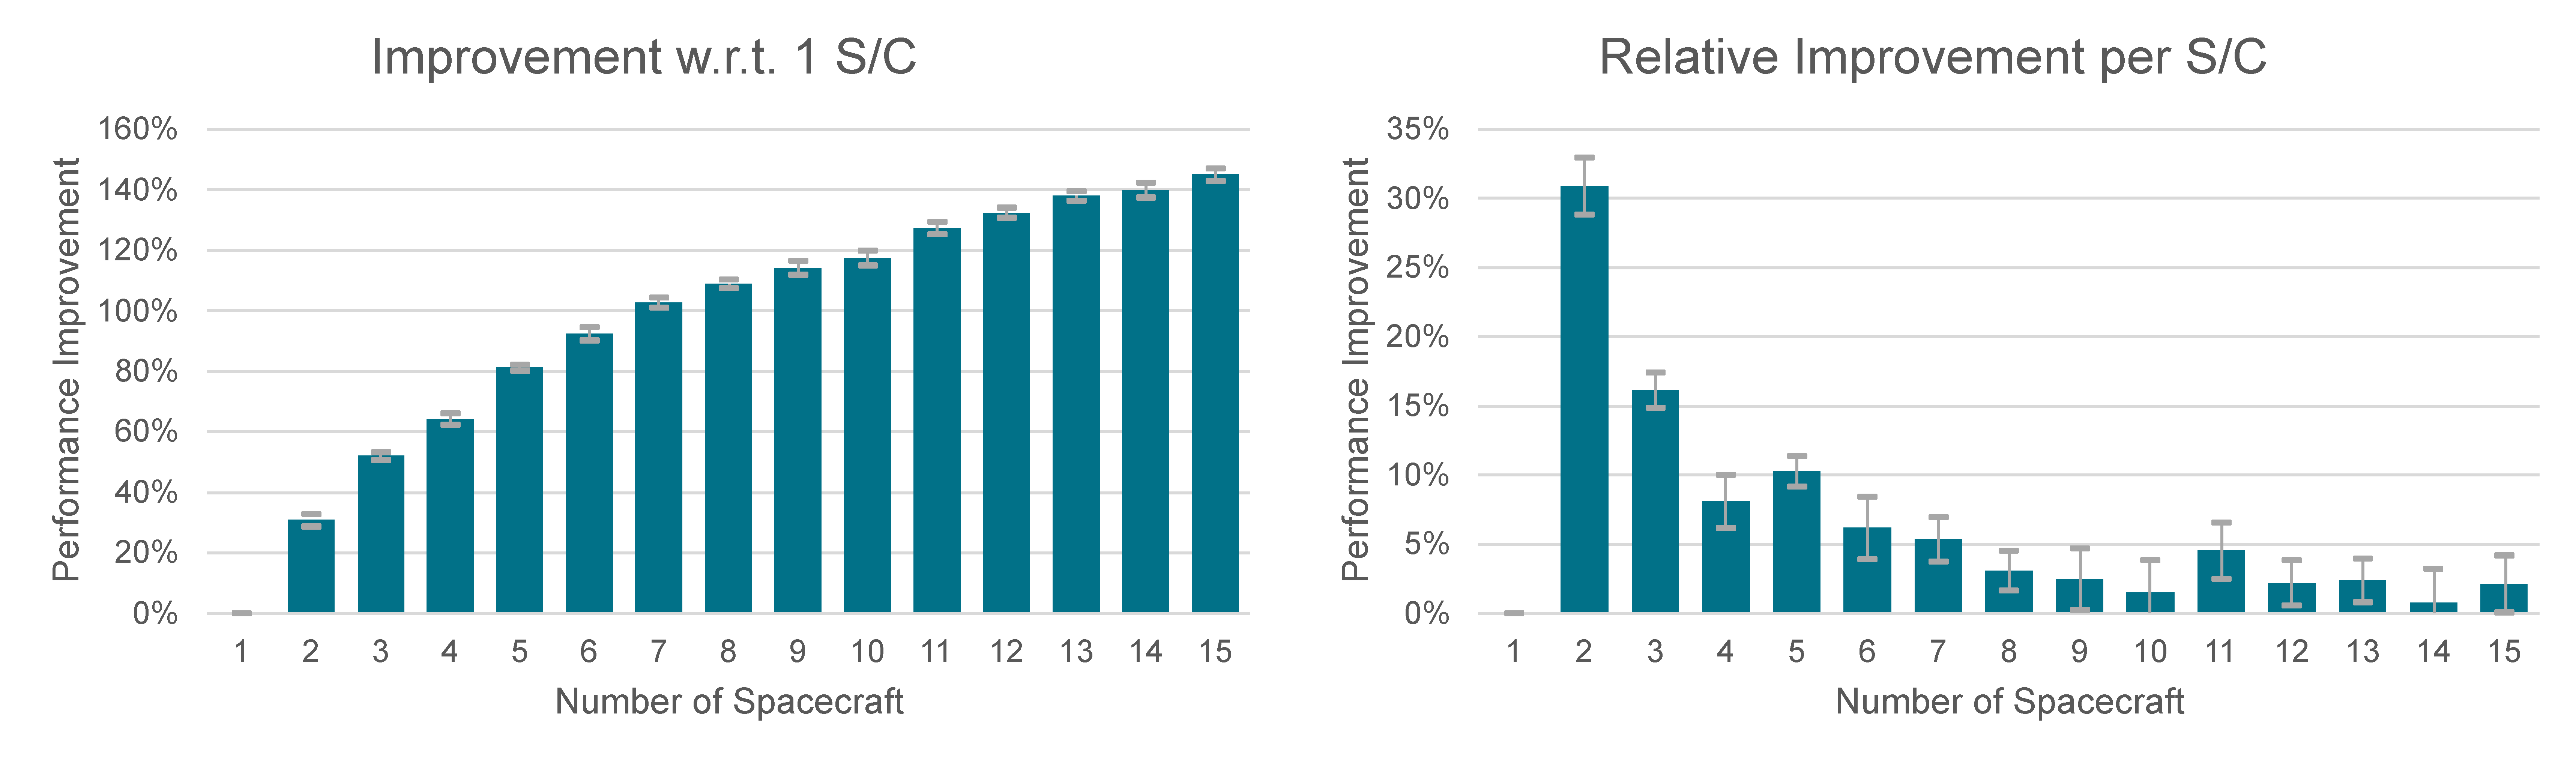
\includegraphics[width=1.0\textwidth]{img/number_sc_tir.pdf}
 \caption{Improvement in survey completeness gained by increasing the number of spacecraft in a purely thermal infrared wavelength system, including standard deviation bars (from 10 iterations). The left graph shows the improvement of an $n$-spacecraft system with respect to a system of a single spacecraft, the right graph shows the improvement of an $n$-spacecraft system with respect to an $n-1$-spacecraft system.}
 \label{fig:results_number_tir}
\end{figure}

As explained previously, the number of spacecraft in the system is a parameter that does not have an optimum with respect to the obtained survey completeness: adding additional spacecraft will logically never degrade the performance of the system. However, in practice other constraints (primarily economical) will be present. Therefore, the increase in performance resulting from such an increased investment is of particular interest. \autoref{fig:results_number_vis} and \autoref{fig:results_number_tir} show the performance increase obtained as a function of the number of spacecraft, for the visual spectrum and thermal infrared, respectively. All results were obtained using the optimal orbital elements deduced in the previous section. Several observations can be made, which will be listed and subsequently discussed below.\\

Firstly, significant diminishing returns present themselves for both spectra; the additional value of an extra spacecraft decreases exponentially with the number of spacecraft already present in the system. Performance increases gained per additional spacecraft fall to around 5\% when surpassing 5 spacecraft in the system. Beyond 10 spacecraft, the increases start to become smaller than the standard deviation in the results. This means that, although large initial improvements in performance can be gained from utilizing a multi-spacecraft system, simply increasing the number of survey spacecraft can not bring us arbitrarily close to 100\% survey completeness; when increasing beyond approximately 5 spacecraft, it is recommended to focus efforts on improving other areas of the system for the mission to remain efficient. \\

This fact compounds the second finding: even the most efficient addition - adding a second spacecraft to a single spacecraft survey system - does not come close to increasing the system performance by 100\%. In other words: increasing the number of spacecraft will \textit{decrease} the number of asteroids detected \textit{per spacecraft}. While this finding might seem irrelevant from a mission design point-of-view - the overall performance still increases - it is nevertheless important to consider in the context of other mission constraints, such as budget. \\

The third result is that thermal infrared systems feature a larger relative improvement to survey performance as the number of spacecraft increases, i.e. thermal infrared systems benefit more from additional spacecraft. This trend continues for higher numbers of spacecraft, with thermal infrared systems reaching a 100\% improvement around 7-8 spacecraft, compared to visual light systems requiring 15-16 spacecraft to achieve a similar performance gain. This, combined with the fact that thermal infrared systems have been shown to be the best choice for future NEA missions using a single spacecraft (see e.g. \cite{2017NEOSDT}, \cite{ThesisOlga}), suggests a multi-spacecraft system should also comprise thermal infrared telescopes. This will be investigated in more detail in \autoref{sec:results_payload}.\\

Finally, it is evident that a variance of around 1-2\% is present in the survey performance results, relative to a smooth exponentially decreasing curve. It was found that this variance is also present when repeatedly sampling the simulation using the same input parameters. Therfore, in these and subsequent results, it will be assumed that this is simply a result of the stochasticity in the model. Possible other explanations will be ruled out further in \autoref{ch:vandv}.

\section{Payload}
\label{sec:results_payload}
\begin{figure}[htbp]
 \centering
 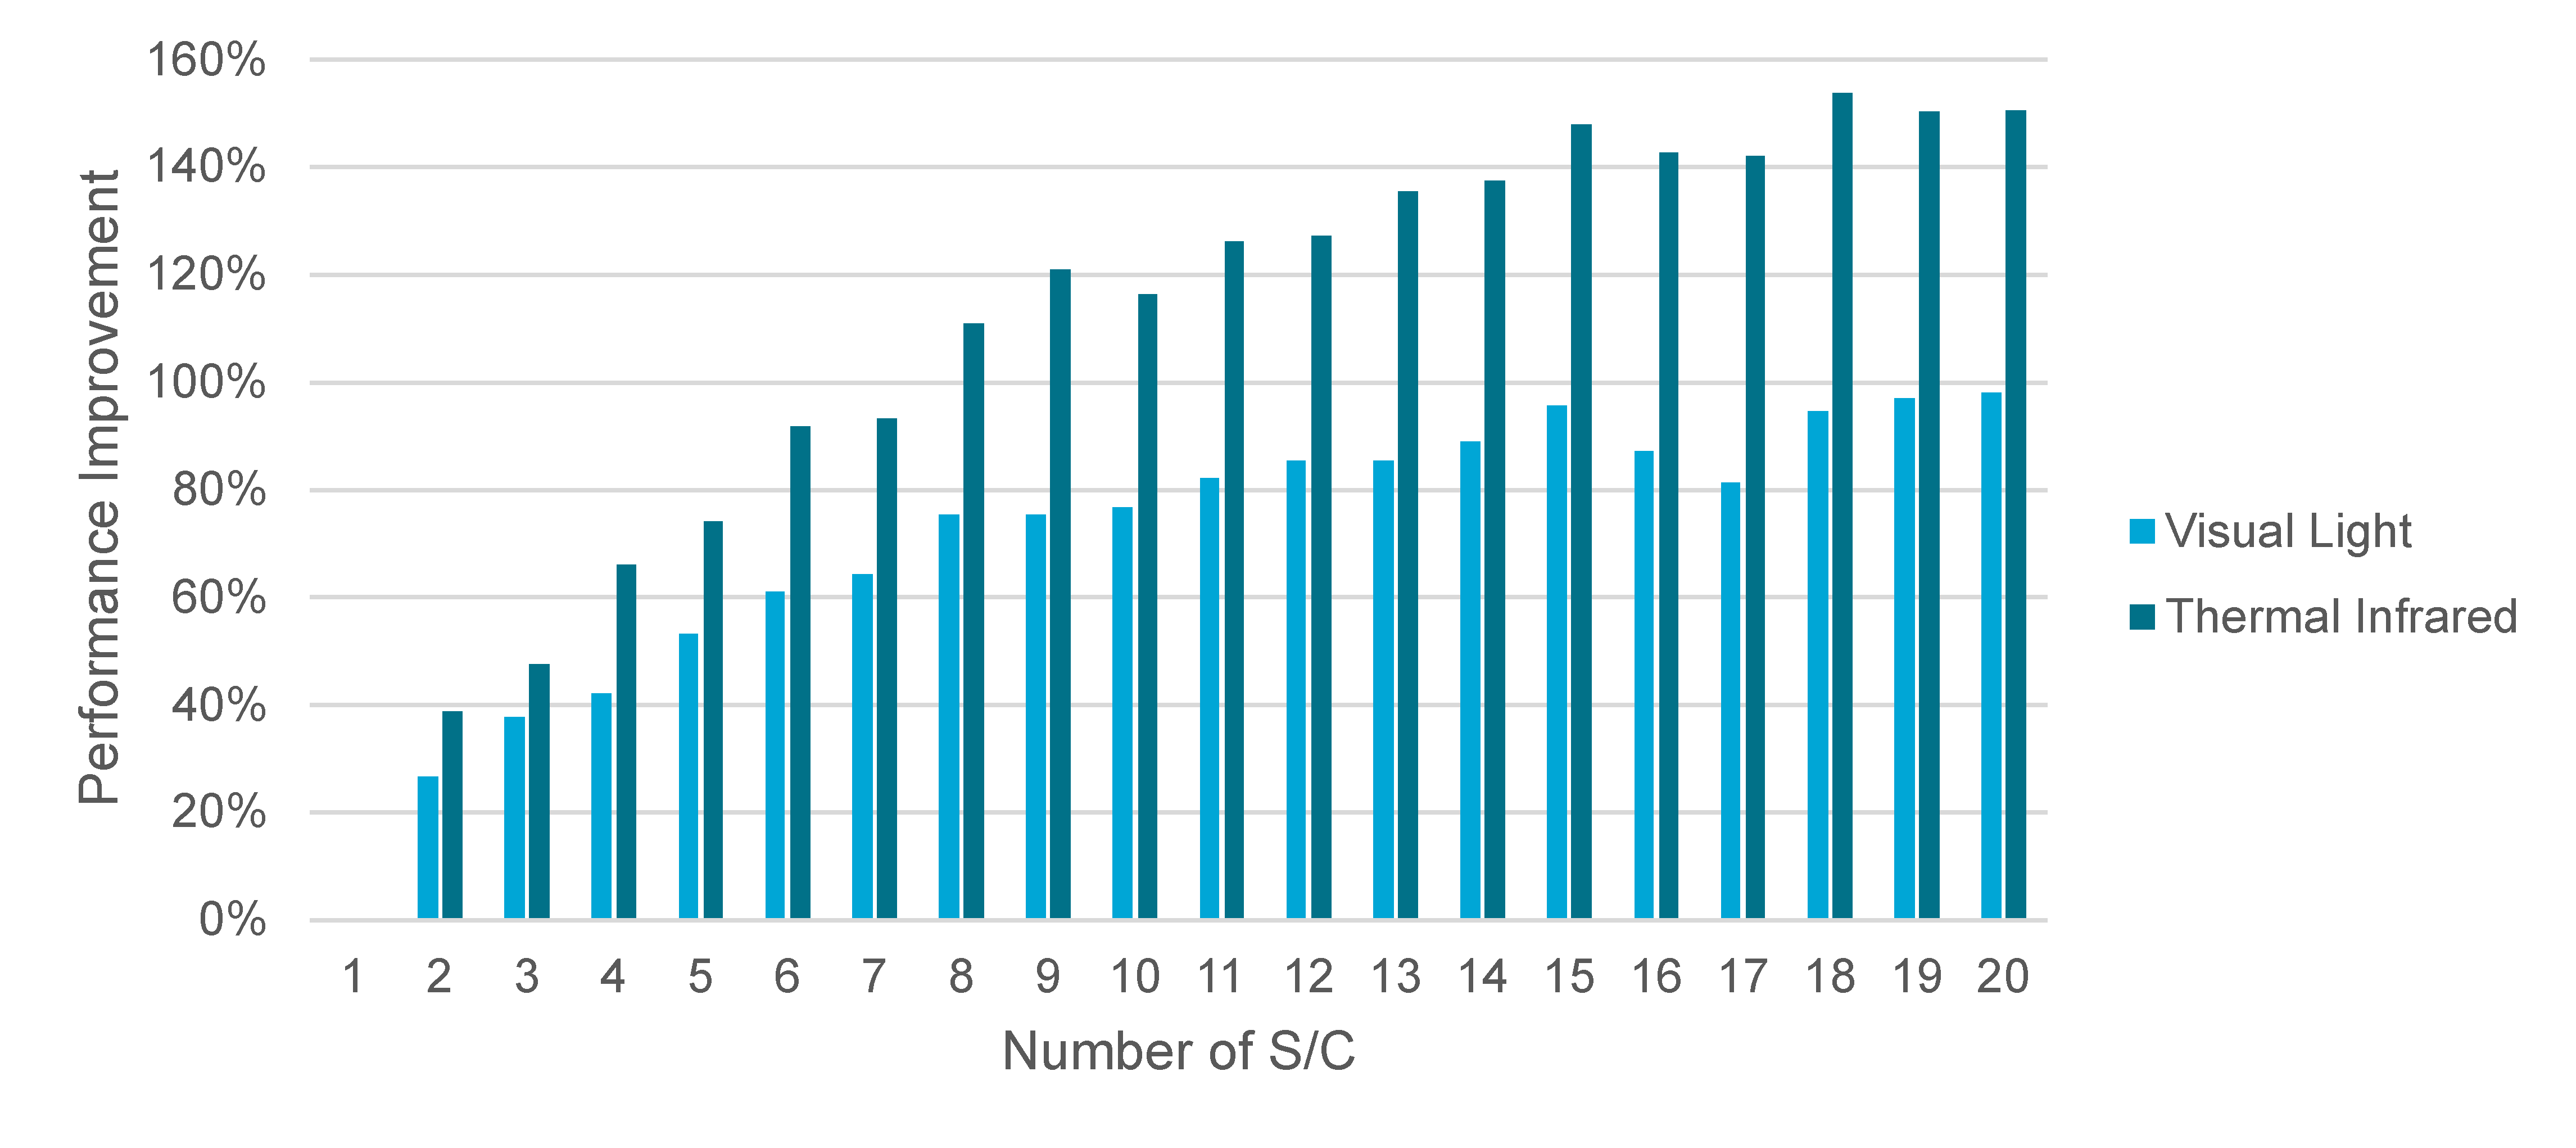
\includegraphics[width=0.8\textwidth]{img/tir_vs_vis_many.pdf}
 \caption{Comparison of relative increase in performance gained relative to a single spacecraft system for visual and thermal infrared systems.}
 \label{fig:tir_vs_vis_many}
\end{figure}

\begin{figure}[htbp]
 \centering
 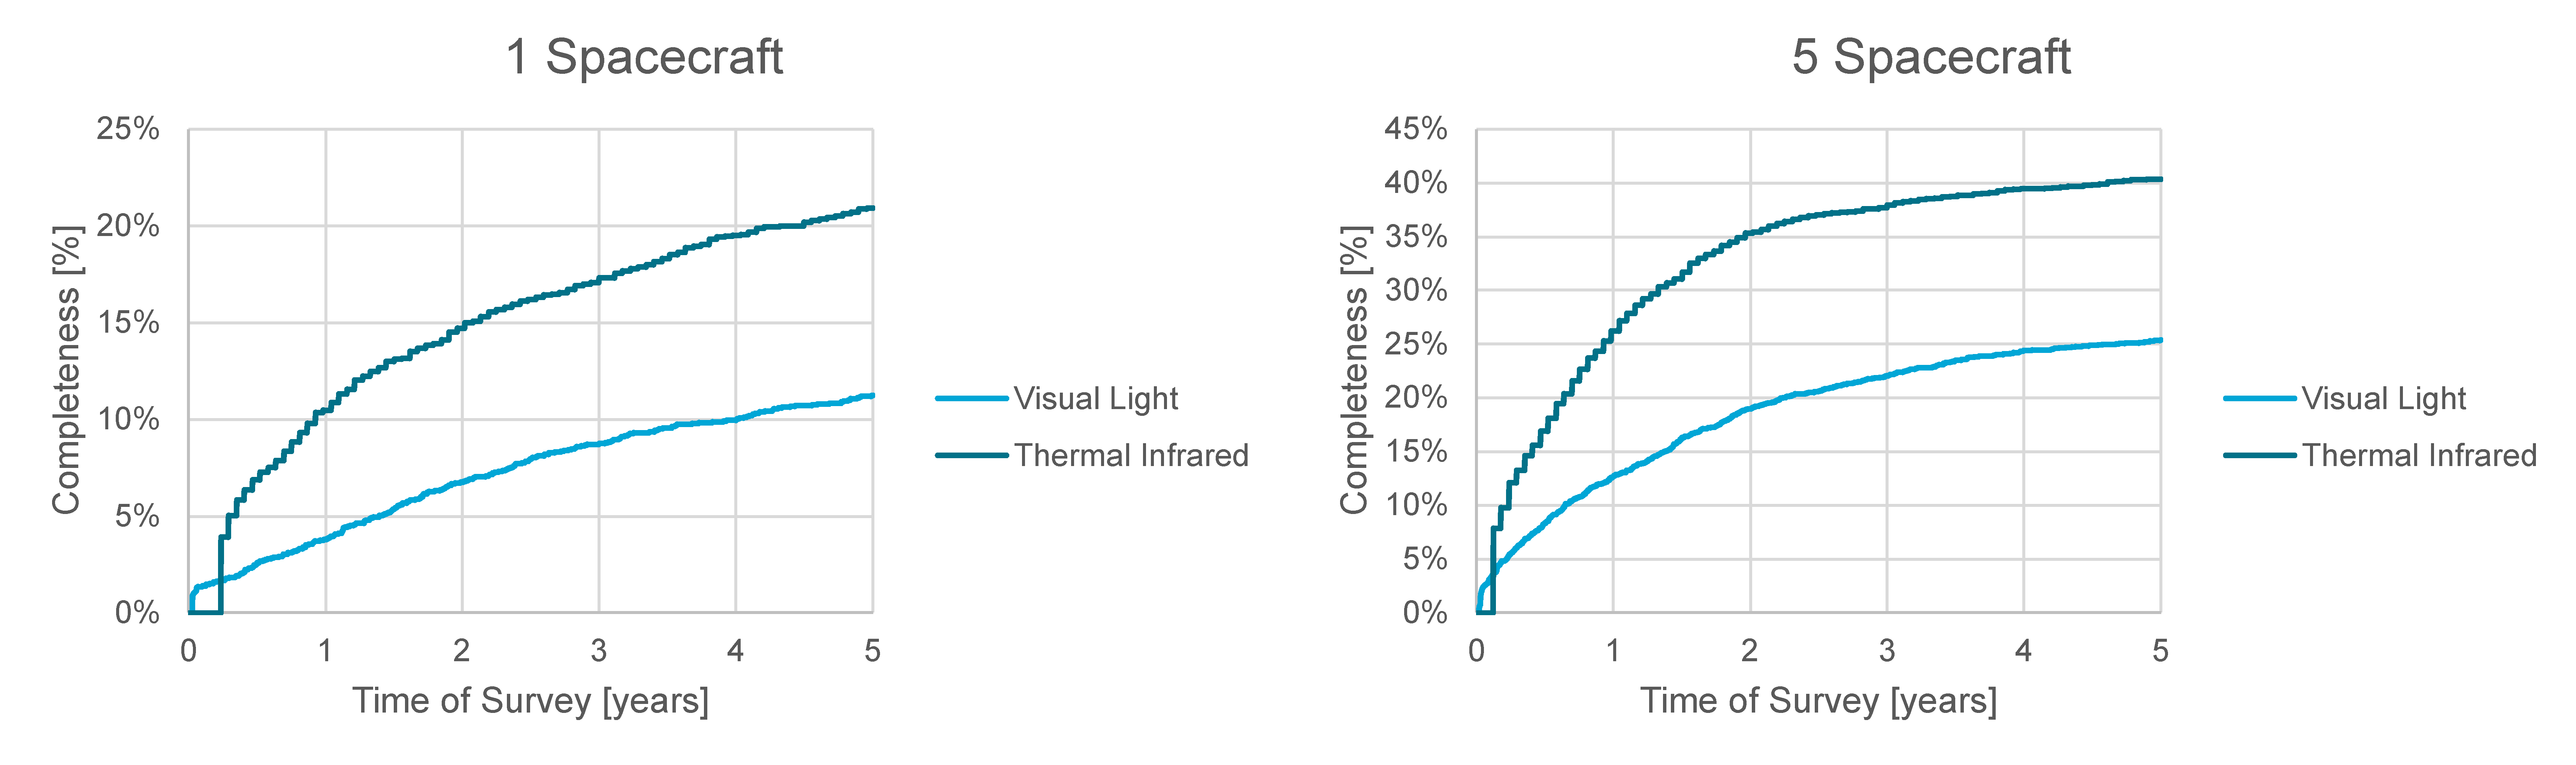
\includegraphics[width=1.0\textwidth]{img/tir_vs_vis_1_5.pdf}
 \caption{Progress of survey completeness over a five year survey for a 1-spacecraft and 5-spacecraft system, in systems where either all spacecraft are equipped with visual light telescopes, or all spacecraft are equipped with thermal infrared telescopes.}
 \label{fig:tir_vs_vis_nohybrid}
\end{figure}


As mentioned in the previous section, initial result suggest thermal infrared systems to be the optimal choice for multi-spacecraft systems because of their predicted higher performance in single-spacecraft systems, and higher benefit from increasing the number of spacecraft. The latter effect is shown in \autoref{fig:tir_vs_vis_many}. In this section, the payload composition will be investigated in more detail. Particular interest is placed in the performance as a function of time - visual light systems feature a faster cadence - and in possible synergistic effects in systems featuring both visual light and thermal infrared telescopes. When interpreting the results of this chapter, it is important to keep in mind the fact that these simulations were carried out assuming contemporary hardware (as listed in \autoref{tab:hardwareproperties}). Advances in either type of telescope or sensor might warrant a future reassessment.\\

Firstly, the performances for systems featuring only one payload type were modelled. For comparison, this analysis was carried out for a 1-spacecraft and a 5-spacecraft system. Because, as shown in the previous section, the payload types exhibit similar behavior when the number of spacecraft is altered, this was assumed to be representative of other numbers of spacecraft as well. The resulting survey performance as a function of time can be seen in \autoref{fig:tir_vs_vis_nohybrid}. Note that, contrary to previous figures, these graphs show the \textit{absolute} survey completeness, not the completeness relative to a benchmark. In the results, it can be observed that initially, the visual light system features a higher completeness due to its faster cadence. However, the thermal infrared system quickly surpasses it as time progresses. This means that the faster cadence granted by the lower integration times and larger sensor sizes of the visual light system does not weigh up to the increased sensitivity of the thermal infrared system on the timescales of survey missions; not only is the final survey completeness more than 10\% higher for a thermal infrared system, it also manages to achieve the same performance as a 5-year visual light survey in only a single year in both examined cases. This agrees with the findings of \cite{ThesisOlga} that for systems where quick detections are important, such as impact last-warning, thermal infrared is also a superior option. \\

\begin{figure}[htbp]
 \centering
 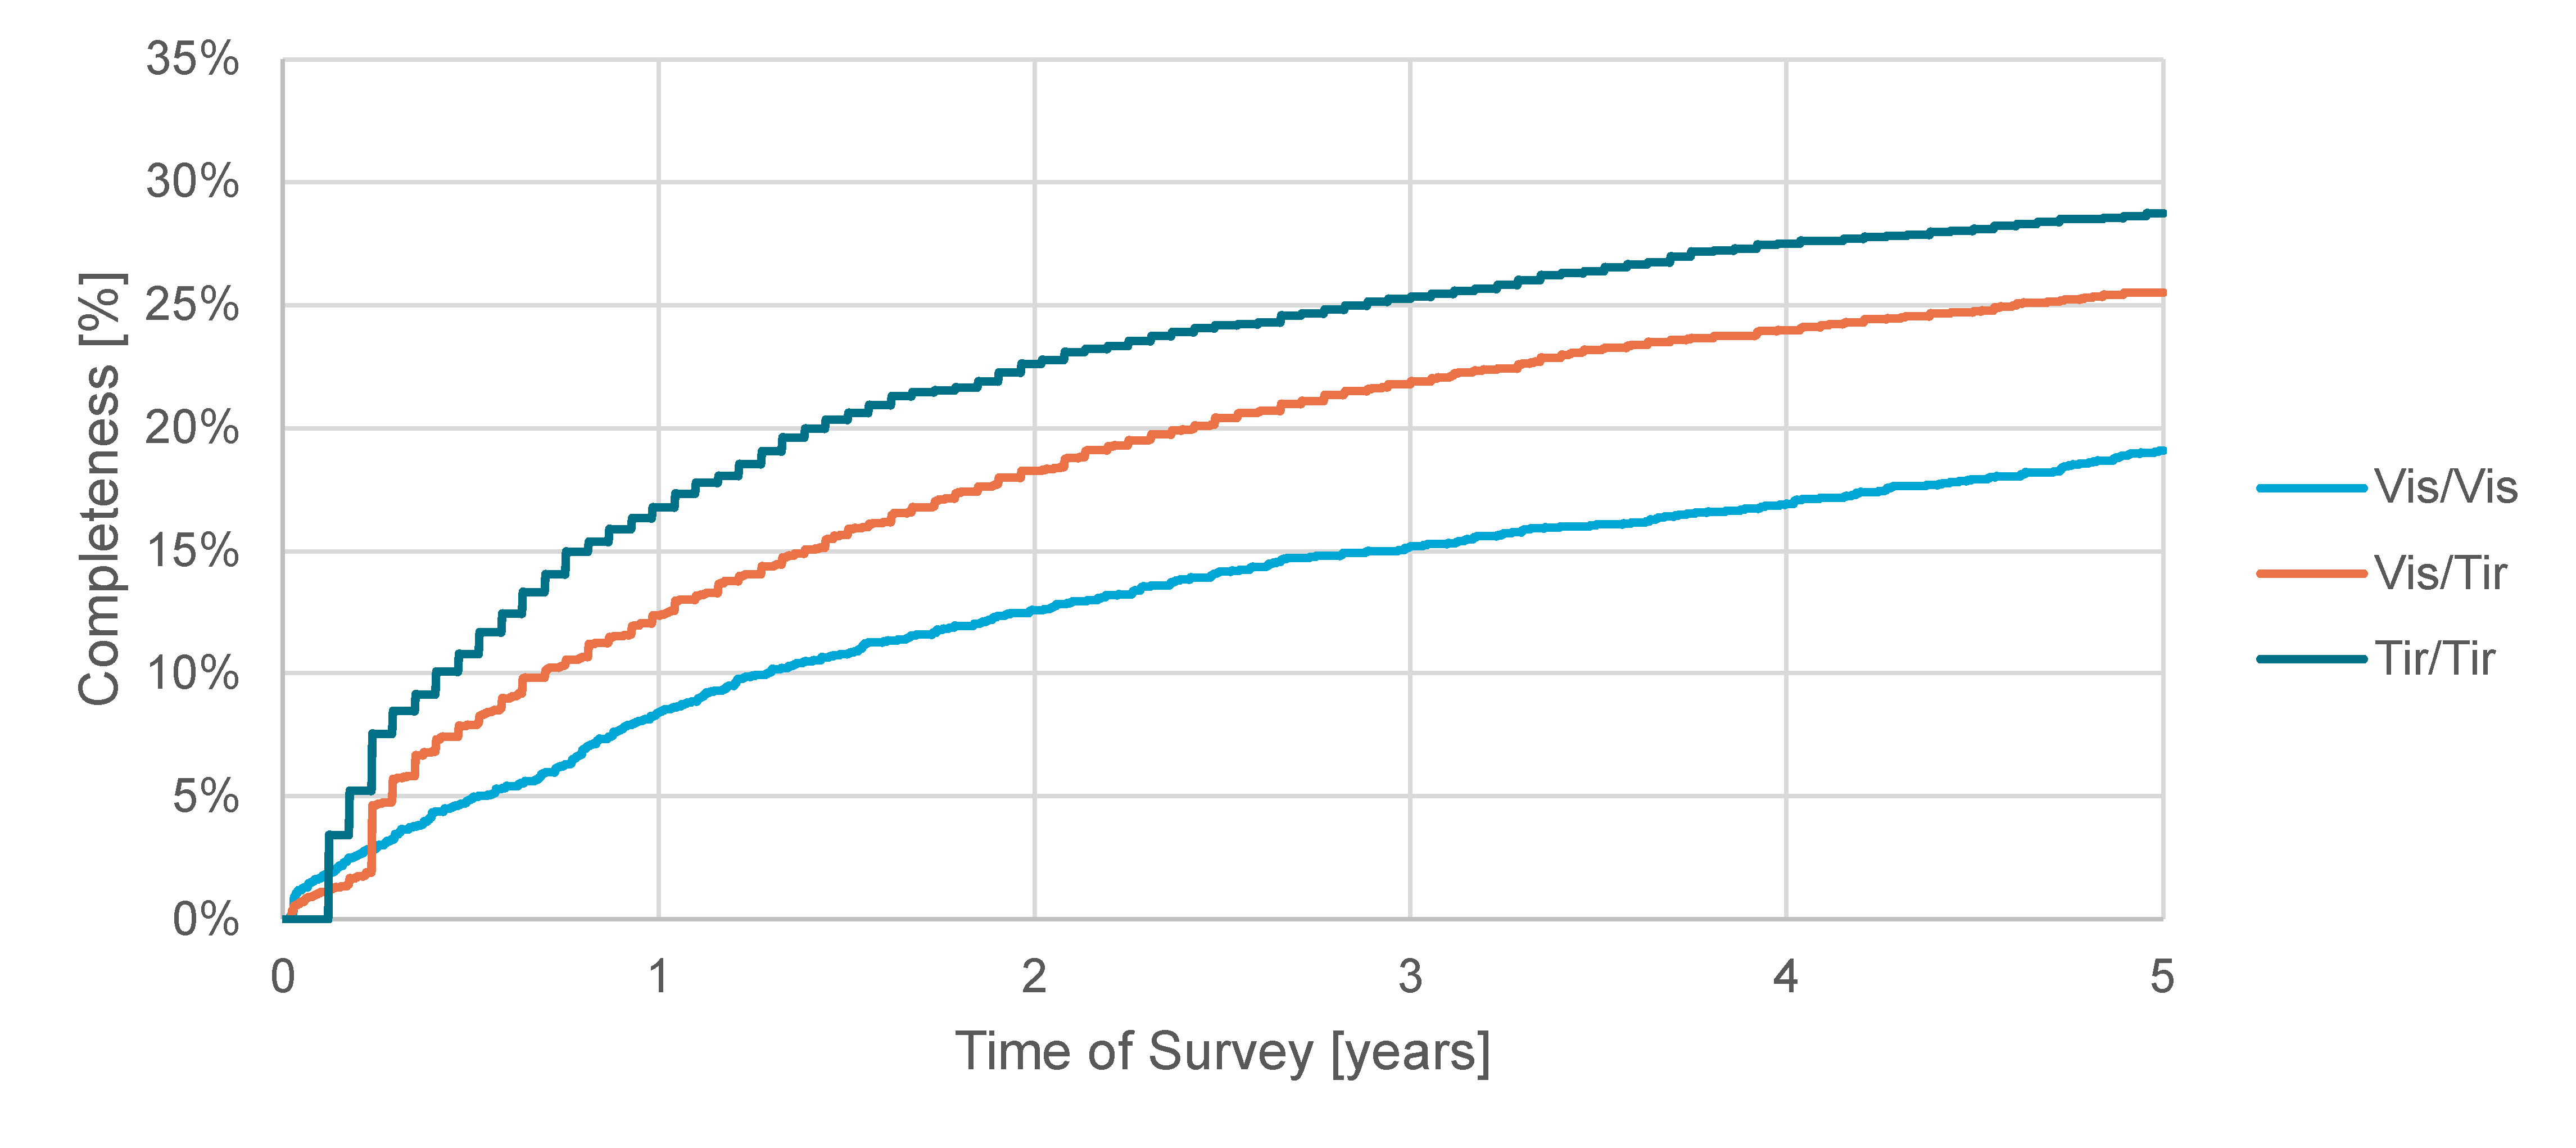
\includegraphics[width=0.8\textwidth]{img/tir_vs_vis_2_hybrid.pdf}
 \caption{Progress of survey completeness over a five year survey for all possible payload combinations in a 2-spacecraft system.}
 \label{fig:payload_hybrid_one}
\end{figure}

\begin{figure}[htbp]
 \centering
 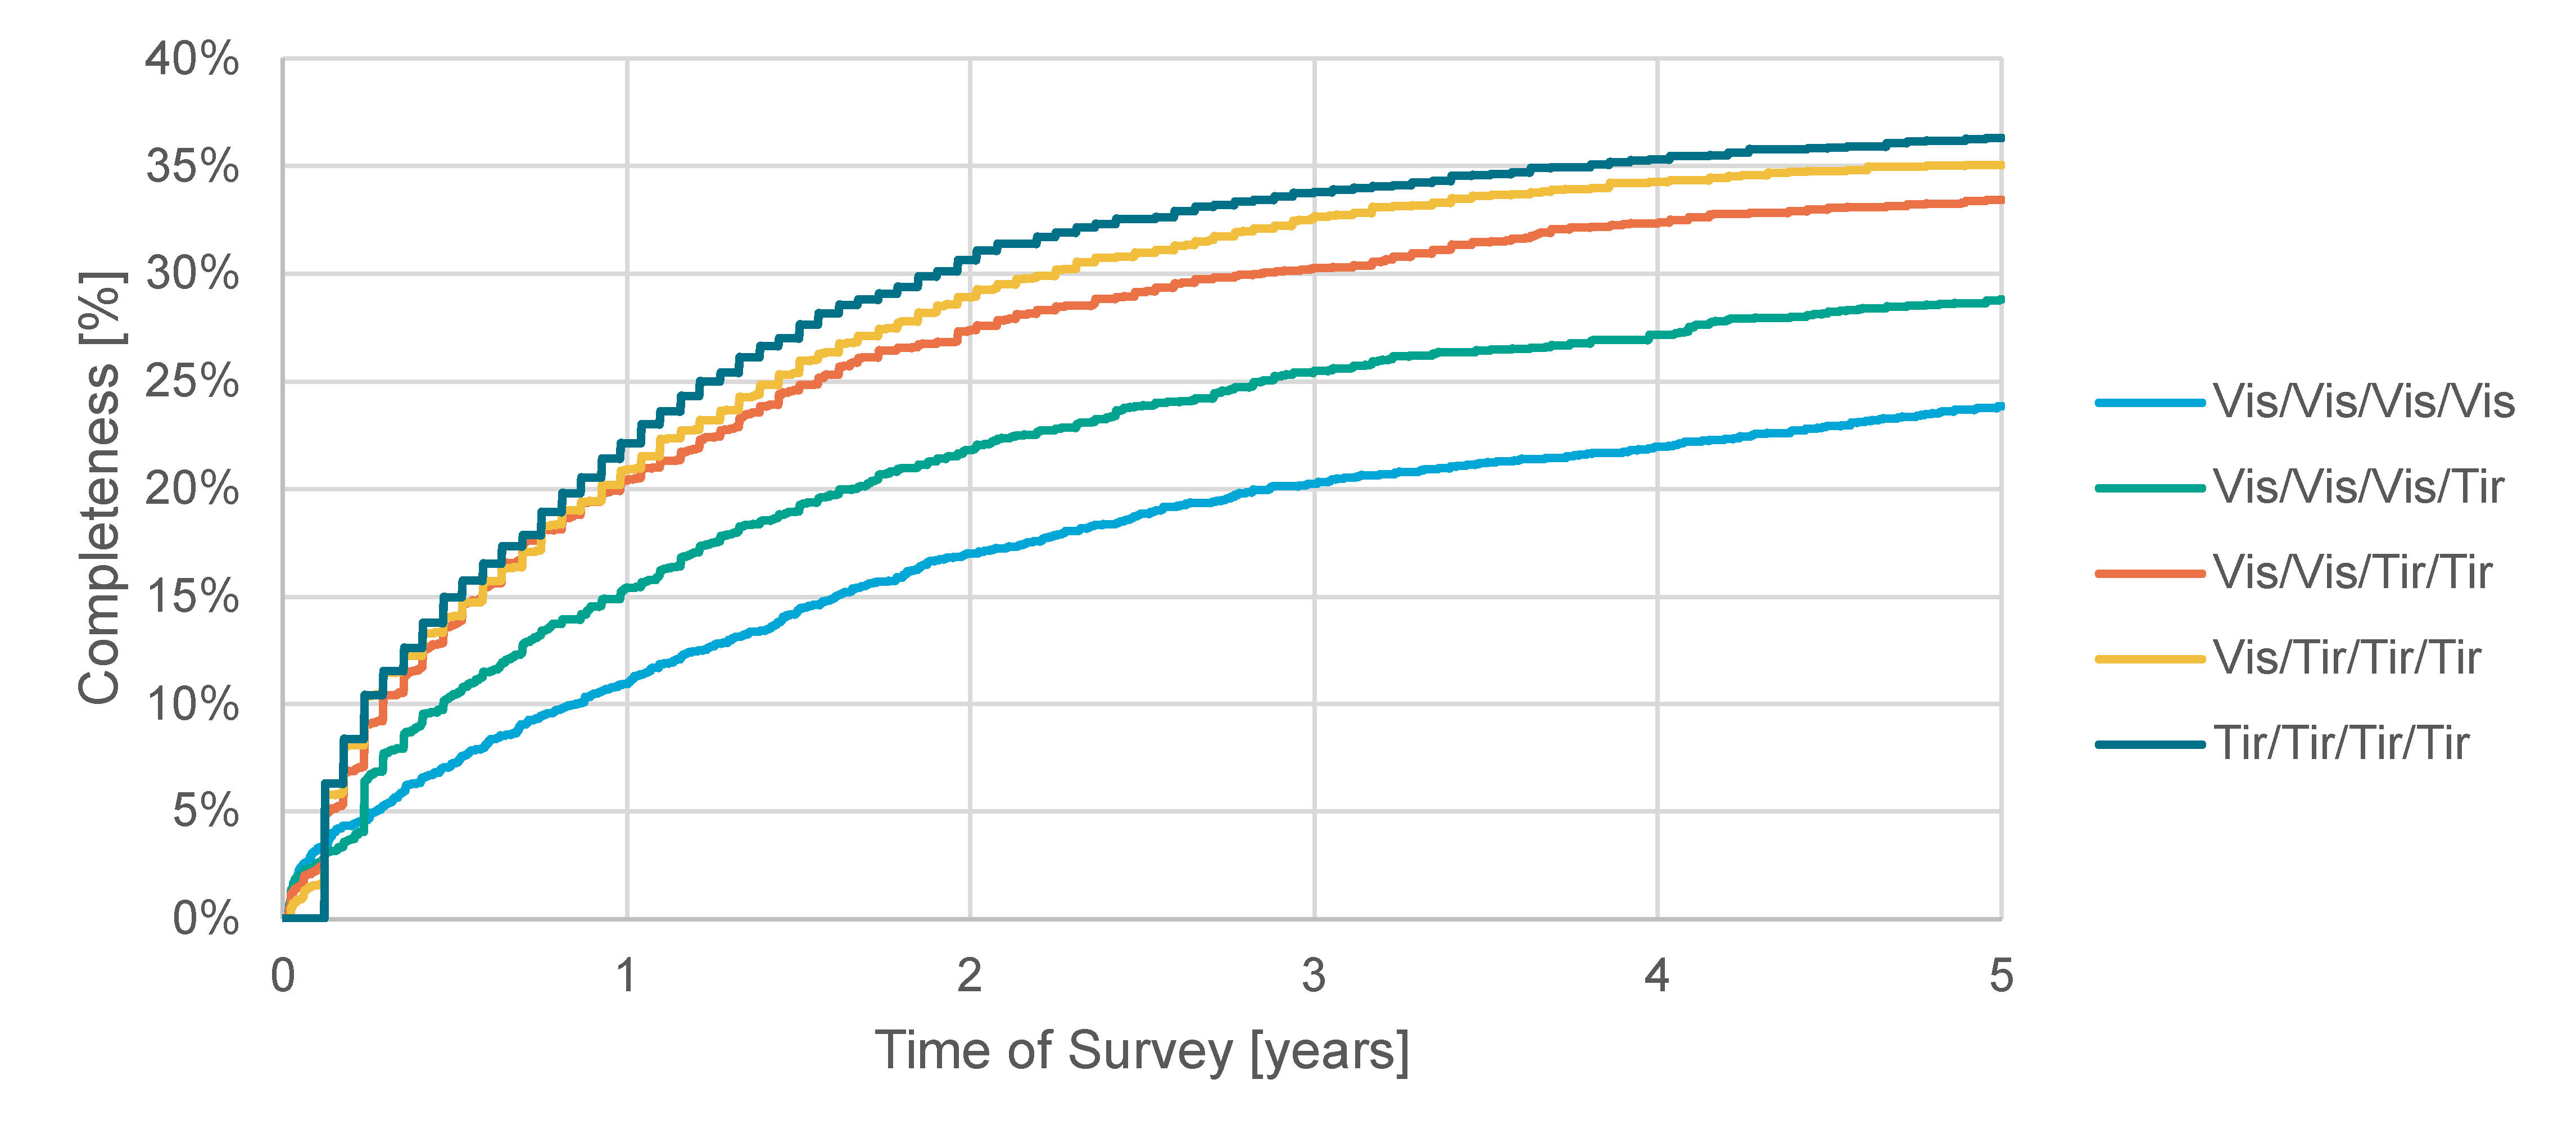
\includegraphics[width=0.8\textwidth]{img/tir_vs_vis_4_hybrid.pdf}
 \caption{Progress of survey completeness over a five year survey for all possible payload combinations in a 4-spacecraft system.}
 \label{fig:payload_hybrid_two}
\end{figure}

In continuation of the payload analysis, systems utilizing a combination of visual light and thermal infrared telescopes were examined. The reasoning is that the higher sensitivity of thermal infrared systems combined with the higher cadence of visual light systems might result in a synergistic effect where the system performs better than the performance of the individual components would suggest. However, as can be seen from the results for 2- and 4-spacecraft systems in \autoref{fig:payload_hybrid_one} and \autoref{fig:payload_hybrid_two}, respectively, this is not the case. A system comprising purely infrared telescopes yields the best results, and performance increases progressively as the number of thermal infrared telescopes in the system increases. This means that in general thermal infrared is the preferred payload type for deep space multi-spacecraft systems aimed at increasing the survey completeness. Note however that this assertion is made under the assumption of a simplistic search strategy, where the system repeatedly images the entire sky. Possible applications of fast visual light telescopes as follow-up telescopes - as demonstrated by the Catalina Sky Survey - might still be a feasible option, although this would first require research into such advanced search strategies.



\section{Explanation of Observed Phenomena}
\label{sec:results_explanation}
To complement and support the previously obtained results, in this section an explanation is proposed to the observed phenomena. Specifically, an attempt will be made to explain the performance increase gained by spreading the spacecraft apart, the increase in optimal semi-major axis as a function of number of spacecraft, and the fact that eccentric orbits yield worse results. In addition, an hypothesis will be drafted for the performance of the non-co-orbital systems, which are analysed in the next section. \\

The proposed mechanism which drives the witnessed performance is through the volume of space which can be covered by the telescope. In other words: A system which can obtain a good SNR on targets in a larger volume of space will outperform a system which has a smaller area where that SNR can be achieved. Simulations were performed on the ecliptic plane, from -5 to +5 AU in both directions, and the limiting magnitude required to achieve an SNR $\geq$ 5 was determined for each point on the plane. \autoref{fig:coverageexplanation} shows an example calculation, with annotation to aid in understanding the illustration. Next to the Sun, spacecraft, and the spacecraft's orbit, the graph shows \textit{the limiting absolute magnitude} (i.e., the smallest NEA) which can be detected at SNR $\geq$ 5 at a specified location.\\

\begin{figure}[htbp]
 \centering
 \includegraphics[width=0.8\textwidth]{img/coverage_explanation_text.png}
 \caption{Explanation of the resulting diagram of coverage area. The color of the area indicates the limiting absolute magnitude of NEA which can still be successfully detected in a given area. Also shown are the Sun, spacecraft, and the orbit of the spacecraft. Several expected phenomena are indicated in the image. Coordinates in the $e$ frame, viewing in the negative $Z_e$-direction.}
 \label{fig:coverageexplanation}
\end{figure}


\begin{figure}[htbp]
 \centering
 \includegraphics[width=1.0\textwidth]{img/coverage_spread.png}
 \caption{Illustration of the observable area for a system of 1, 3 and 5 spacecraft, spread out over the orbit. Coordinates in the $e$ frame, viewing in the negative $Z_e$-direction.}
 \label{fig:coverage_spread}
\end{figure}

In \autoref{fig:coverage_spread} the results of this simulation can be seen for 1, 2 and 5 spacecraft in a 1 AU circular orbit, spread out equally. Several things should be noted about the results here before continuing: Firstly, it can be seen that increasing the number of spacecraft allows for covering the ``blind spots'' caused by Solar glare already at low numbers of spacecraft. The blind area in line with the Sun which can be seen in the diagram with only a single spacecraft is almost completely covered by three spacecraft. Secondly, already at low numbers of spacecraft, a large area is covered at low absolute magnitude (i.e., large asteroids). Lastly, asteroids with a high absolute magnitude (i.e., small asteroids) can only be detected very close to a spacecraft. \\

\begin{figure}[htbp]
 \centering
 \includegraphics[width=1.0\textwidth]{img/coverage_tight.png}
 \caption{Illustration of the observable area for a system of 1, 3 and 5 spacecraft, spread apart by 0.2 rad ($\approx 11.5^\circ$). Coordinates in the $e$ frame, viewing in the negative $Z_e$-direction.}
 \label{fig:coverage_tight}
\end{figure}


The findings here can be constrasted with the results obtained when the spacecraft are not spread out, as can be seen in \autoref{fig:coverage_tight}. Three things here are noted: the reduction in blind spots is less effective, still leaving a large area obstructed by the Sun. Secondly, the system is no longer capable of detecting large asteroids in almost the entire search volume. The actual size of the ``bubble'' grows only marginally with additional spacecraft. Lastly, even for the areas where small NEAs can be detected, some overlap is present which will also decrease the performance. Therefore, the actual volume where NEAs can be effectively detected is decreased by a sizeable amount when not spreading apart the spacecraft, and the performance gains are instead only caused by an increase in the number of times the sky is imaged (effectively speeding up the cadence).\\

\begin{figure}[htbp]
 \centering
 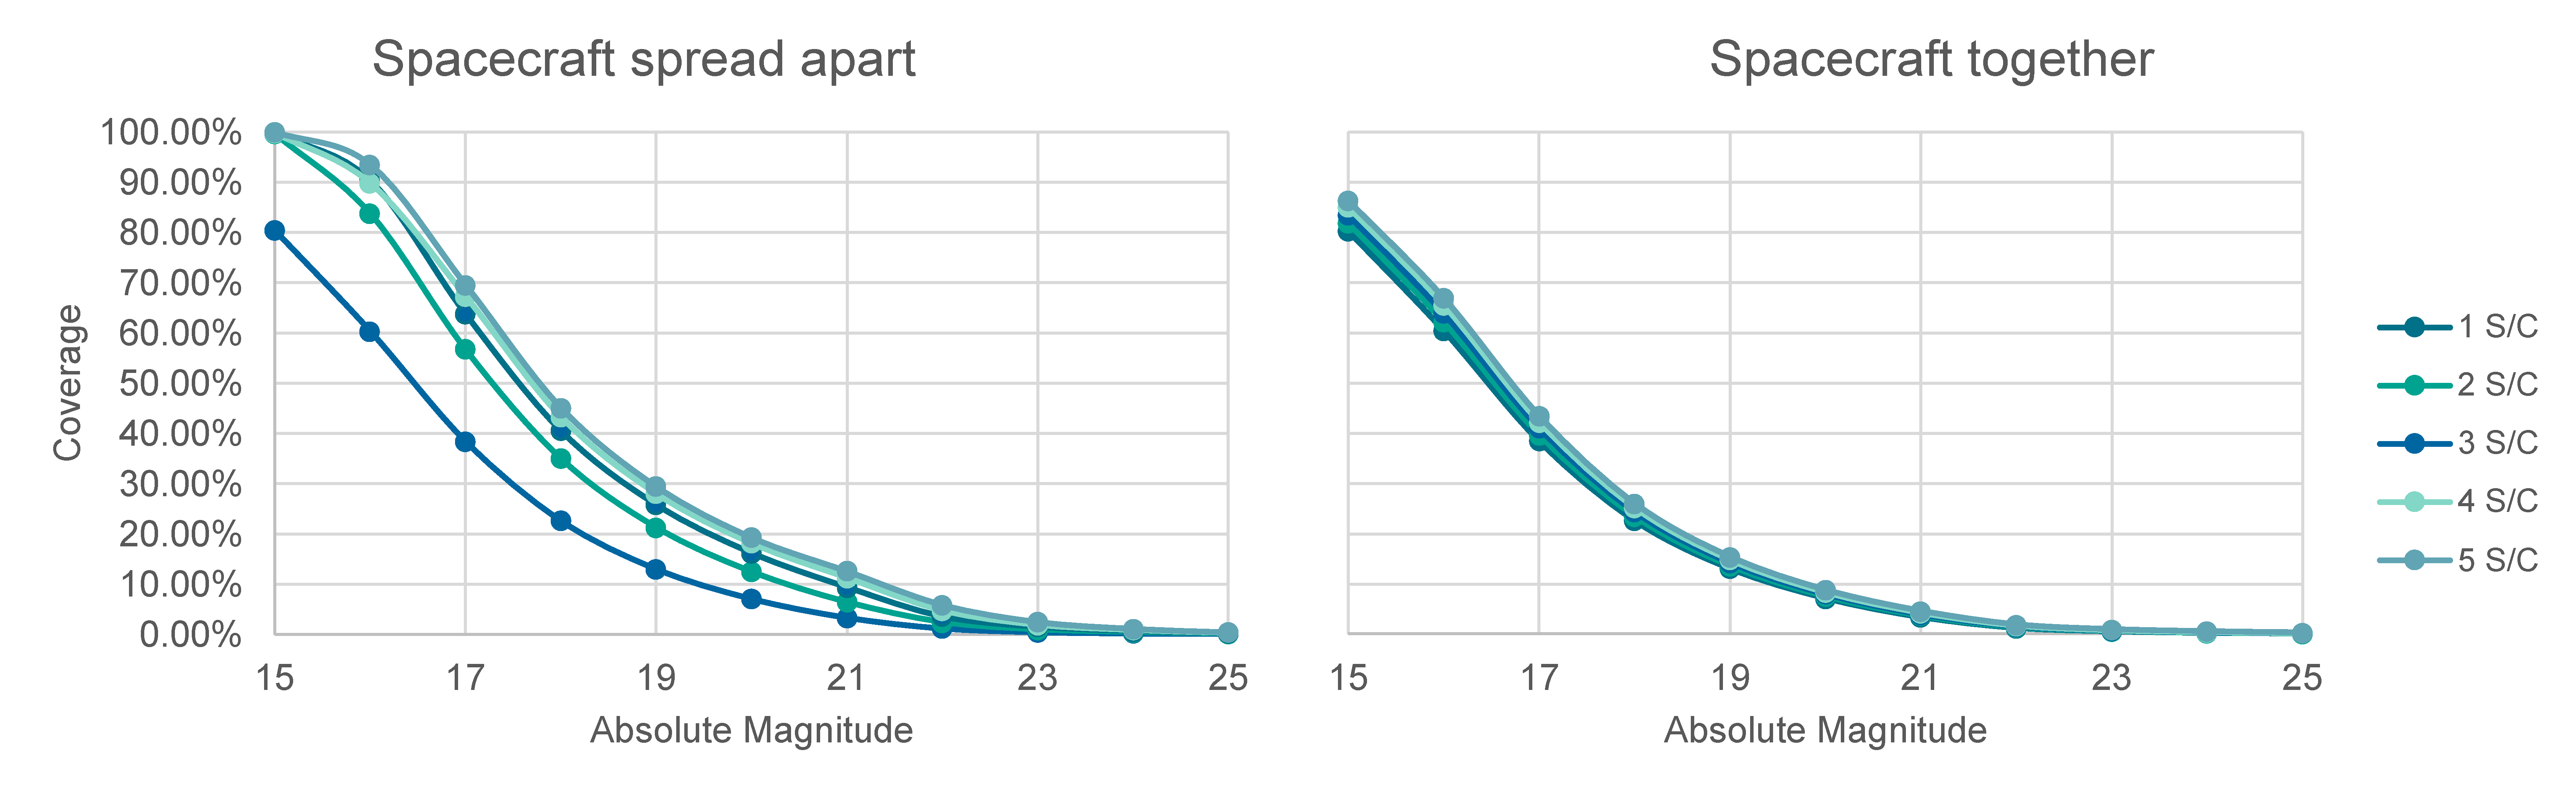
\includegraphics[width=1.0\textwidth]{img/spread_coverage.pdf}
 \caption{Relationship between coverage and asteroid absolute magnitude for spacecraft spread maximally apart, or spread only 0.2 rad}
 \label{fig:spread_coverage}
\end{figure}

The witnessed relationship was investigated numerically, to confirm whether a statistically significant relationship exists, or the effect is merely empirical in nature. For this, a numerical scoring for the coverage was established. This score was set to be the mean of the fraction of the entire area where a certain absolute magnitude can be observed, for absolute magnitude 17-25. That is, with $A_{H}$ the area where an asteroid with absolute magnitude $H$ can be detected at SRN $\geq 5$, and $A_{total}$ the total area, the coverage is defined as:
\begin{equation}
 \mathrm{Coverage} = \frac{1}{25-17}\Sigma_{H=17}^{H=25} \frac{A_{H}}{A_{total}}
\end{equation}
As an example, the coverages at various absolute magnitudes (thus, without the summation) for the above two examples are shown in \autoref{fig:spread_coverage}. It can be seen that indeed, the coverage at all magnitudes is larger for the spread-apart case. And, as established before, the performance is indeed higher for the case with the spacecraft spread apart. To confirm this finding further, a random sampling of a large number of solutions with different semi-major axes, inter-spacecraft spread, and eccentricity, was performed for 2 to 5 spacecraft, and the coverage and completeness was calculated. The results can be seen in \ref{fig:coverage_completeness}. Clearly, a very strong relationship is present between the coverage and the resulting completeness, in addition to a weaker relationship between the number of spacecraft and the completeness (caused by the aforementioned increase in cadence). In other words: the main driver of the survey performance is the volume in space where the system can effectively image asteroids. \\

\begin{figure}[htbp]
 \centering
 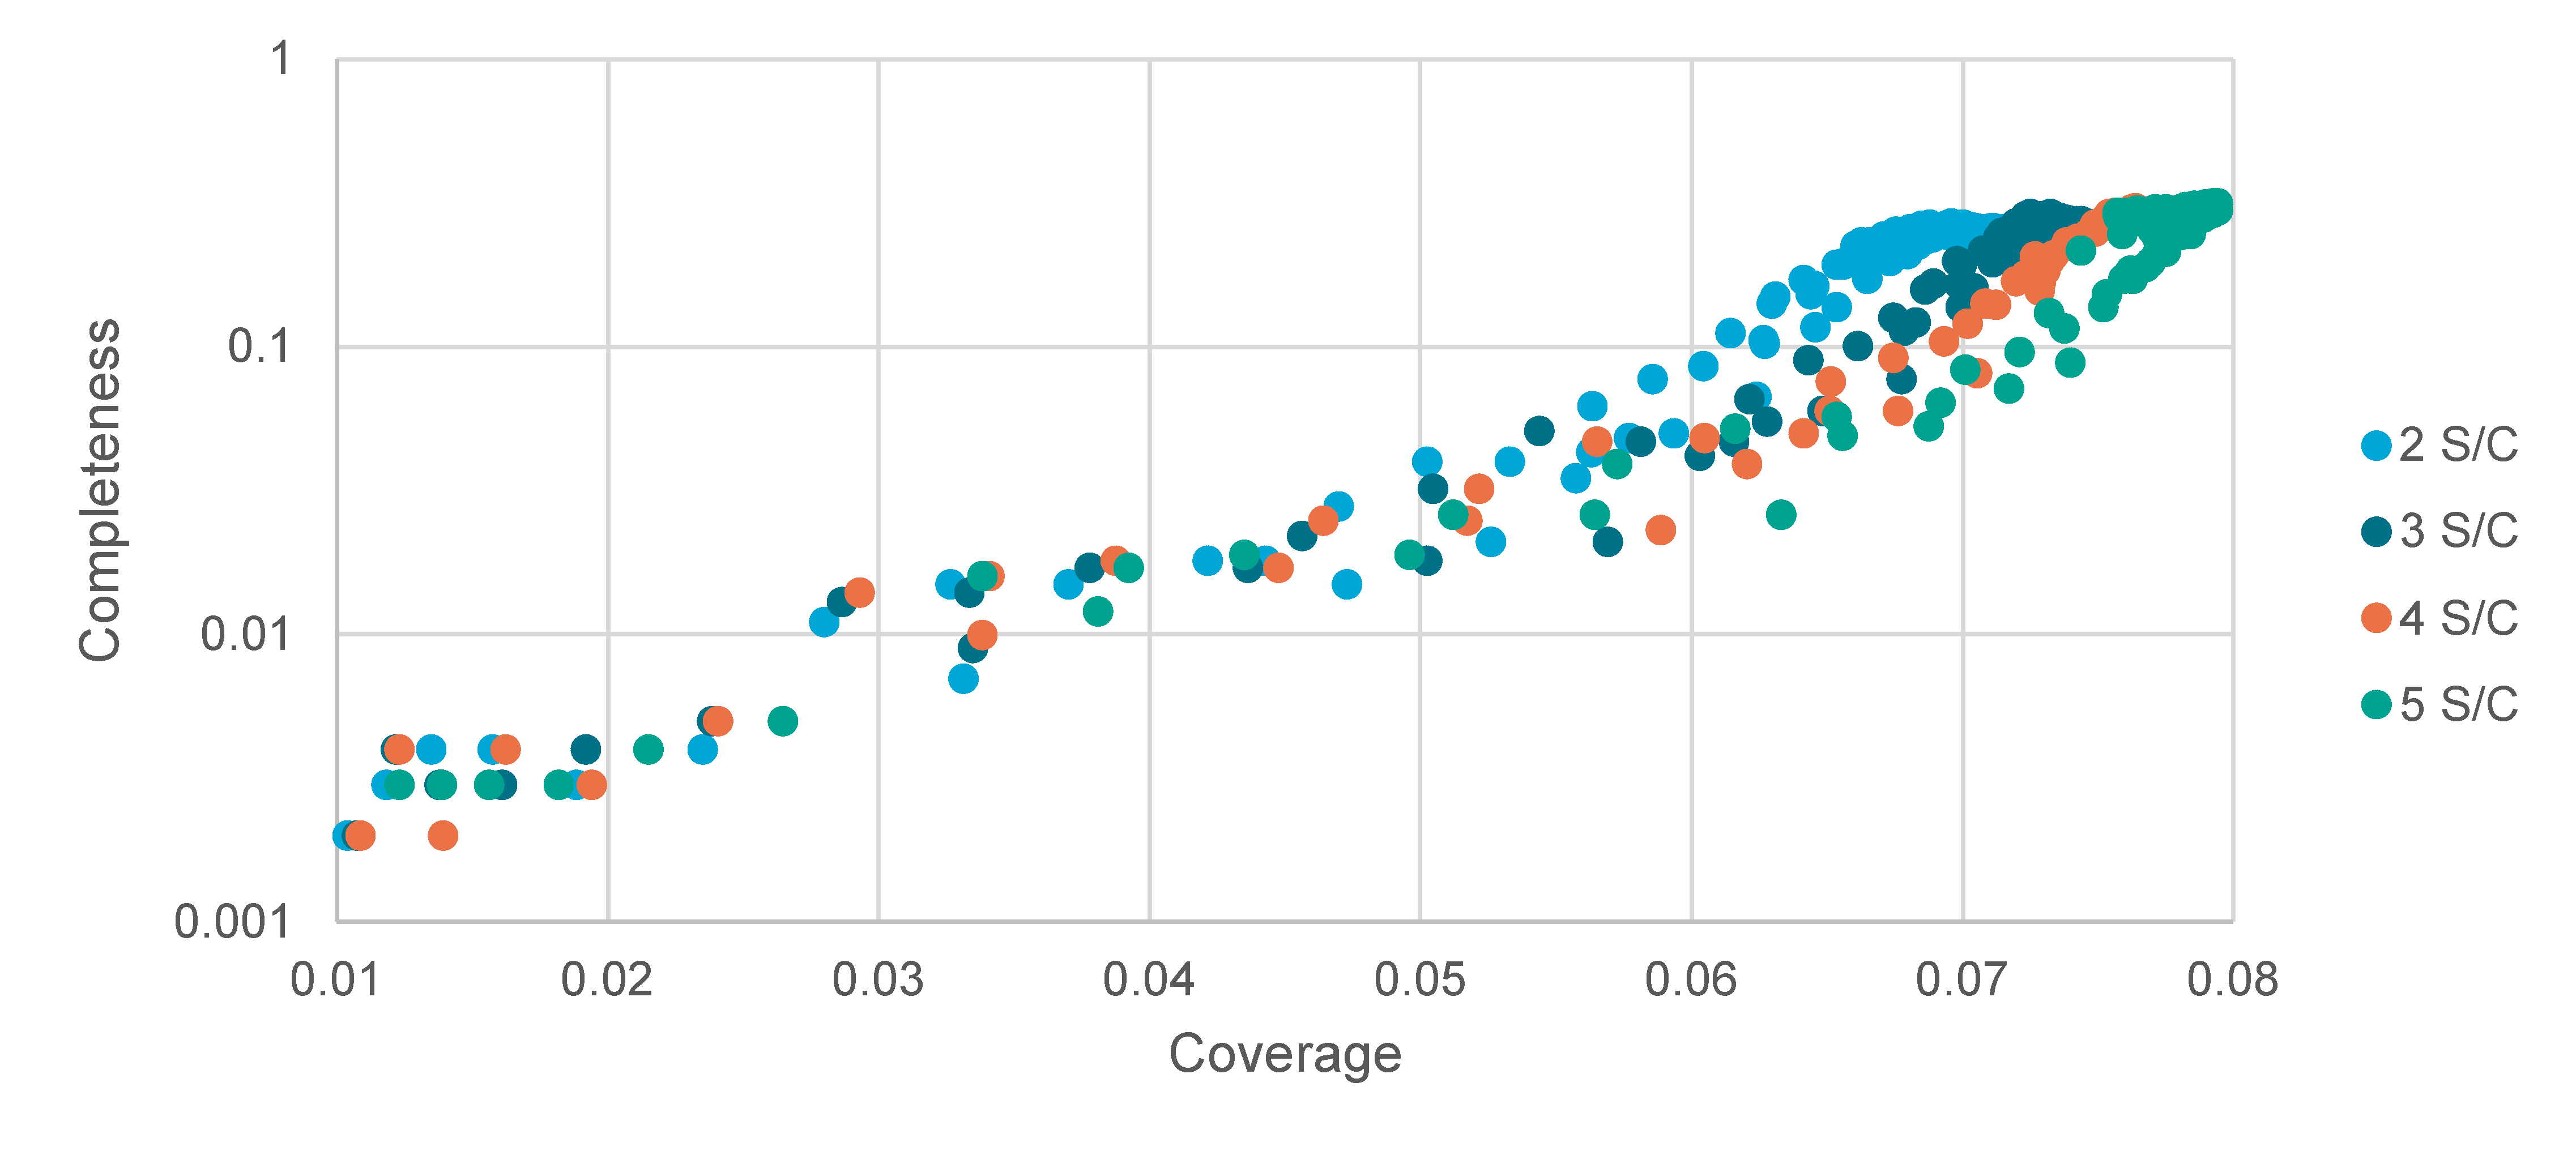
\includegraphics[width=1.0\textwidth]{img/coverage_completeness.pdf}
 \caption{Relationship between coverage and completeness for 2-5 spacecraft. }
 \label{fig:coverage_completeness}
\end{figure}

Working from this relationship, several of the phenomena observed so far can be explained. Firstly indeed the effect of spreading the spacecraft apart as much as possible to minimize the overlap in their search areas. This was already shown previously. Although no statistically significant data is available to confirm this, it is theorized that this is also the reasoning why eccentric orbits do not produce optimal results: As the orbital velocity of the spacecraft is lower near apohelion than near perihelion, the spacecraft in the system will tend to congregate near the apohelion. This then effectively decreases the spread between the spacecraft, increasing the overlap. Secondly, the phenomenon of increasing optimal semi-major axis with larger number of spacecraft can be explained in this way. \autoref{fig:coverage_high_n} shows the resulting coverage for a system of 15 spacecraft, compared to the aforementioned 5 spacecraft, which are shown for reference. It can be seen that as the semi-major axis remains constant, but $n$ increases, a large overlap in the coverage area develops. As the semi-major axis increases, the overlap decreases. Therefore, although individual spacecraft might no longer be in the optimal range, the entire system is capable of detecting asteroids in a larger volume of space, again increasing performance. \\

\begin{figure}[htbp]
 \centering
 \includegraphics[width=1.0\textwidth]{img/coverage_high_n.png}
 \caption{Illustration of the observable area for a system of 15 spacecraft, at a=1.0 AU and a=1.5AU, spread out over the orbit. The 5 spacecraft case is shown for comparison. Coordinates in the $e$ frame, viewing in the negative $Z_e$-direction.}
 \label{fig:coverage_high_n}
\end{figure}

Lastly, this theory can be utilized to provide a prediction about what change in performance is to be expected when optimizing non-co-orbital systems. Such a base prediction is important, as it will help frame the results of the optimizer.  Consider \autoref{fig:coverage_free}: A system is modelled with the semi-major axes of all spacecraft 0.2 AU apart (middle image). Initially, this might seem to cover a larger area than the co-orbital system shown in the left image. Therefore, one would expect it to perform better. However consider the dynamical behavior of the system: As the orbital period of the spacecraft is now different for each spacecraft, they will no longer remain equally spread in space. Over time, spacecraft ``line up'' in a single location, as shown in the right image. It is clear that such a case would be far less preferable than the system in which all spacecraft are situated in the same orbit. Therefore, it is hypothesized that these non-co-orbital solutions will not significantly outperform the co-orbital solutions considered in the previous section.\\

\begin{figure}[htbp]
 \centering
 \includegraphics[width=1.0\textwidth]{img/coverage_free.png}
 \caption{Illustration of the observable area for a system of 5 spacecraft, spread out over the orbit. The left case has the spacecraft co-orbital. In the middle case, the spacecraft are in different orbits, but spread out. On the right, they have lined up in their orbital motion.}
 \label{fig:coverage_free}
\end{figure}

Overall, this theory suggests that the best approach to organizing NEA surveys is to position the spacecraft in such a way as to maximize the volume in which NEAs can be observed. Although this might logically lead to the theory that more complicated orbital arrangements yield better results, this fact is doubtful due to the dynamic behavior of the system reducing the effectiveness over time. One topic here is highlighted which could be investigated for further research: Lagrange points, specifically $L_1$/$L_2$/$L_3$. These points allow the system to utilize slightly different semi-major axes around the Sun, while still maintaining the same orbital periods as other spacecraft in the system, thereby maintaining the distance between the spacecraft. However, due to the additional complication involved in modelling orbits around Lagrange points, modelling of this is left as a recommendation for future research.

\section{Orbital Elements II: Non Co-orbital Spacecraft}
\label{sec:results_orbits_two}

\begin{table}[htbp]
\caption{Overview of optimization parameters for the three investigated optimization cases.}
\label{tab:optimizationcases}
\begin{tabulary}{1.0\textwidth}{L|L|L|L|L}
\textbf{Case}                & \textbf{Semi-major axis}             & \textbf{Eccentricity}            & \textbf{Anomaly at epoch}        & \textbf{Number of parameters} \\ \hline
Circular, co-orbital         & 1 optimization parameter for all S/C & 0                                & Spread evenly over the orbit     & 1                             \\
Circular, non-co-orbital     & 1 optimization parameter per S/C     & 0                                & 1 optimization parameter per S/C & 2n                            \\
Non-circular, non-co-orbital & 1 optimization parameter per S/C     & 1 optimization parameter per S/C & 1 optimization parameter per S/C & 3n
\end{tabulary}
\end{table}

Although the aforementioned analysis predicts a detrimental effect on performance, it is nevertheless logical to extend the analysis presented in \autoref{sec:results_orbits_one} to non-co-orbital configurations. This complicates the analysis significantly, as the dimensionality of the problem rapidly increases. Therefore, special attention has to be paid to the performance of the optimizer, and validation tests should be run on its results. In addition, to aid in comparison, three sets of optimization parameters were analysed. Firstly, a circular, co-orbital case: a system which has all spacecraft spread out as much as possible, in a single circular orbit. From the results in the previous section, it follows that this is the optimal co-orbital solution. Secondly, a circular, non-co-orbital case: a system in which each spacecraft can have a distinct semi-major axis and anomaly at epoch. Because spacecraft with different semi-major axes have different orbital periods, the spacecraft can not be spread out equally a priori. Therefore, the optimizer has to take care of this task as well, and not just the semi-major axes. Lastly, a non-circular, non-co-orbital case: a similar set of parameters is analysed, but with orbits that are allowed to be non-circular. In that case, the parameter space comprises a semi-major axis, true anomaly at epoch, and eccentricity for each spacecraft. An overview of the different optimization cases is given in \autoref{tab:optimizationcases}.\\

\begin{figure}[htbp]
 \centering
 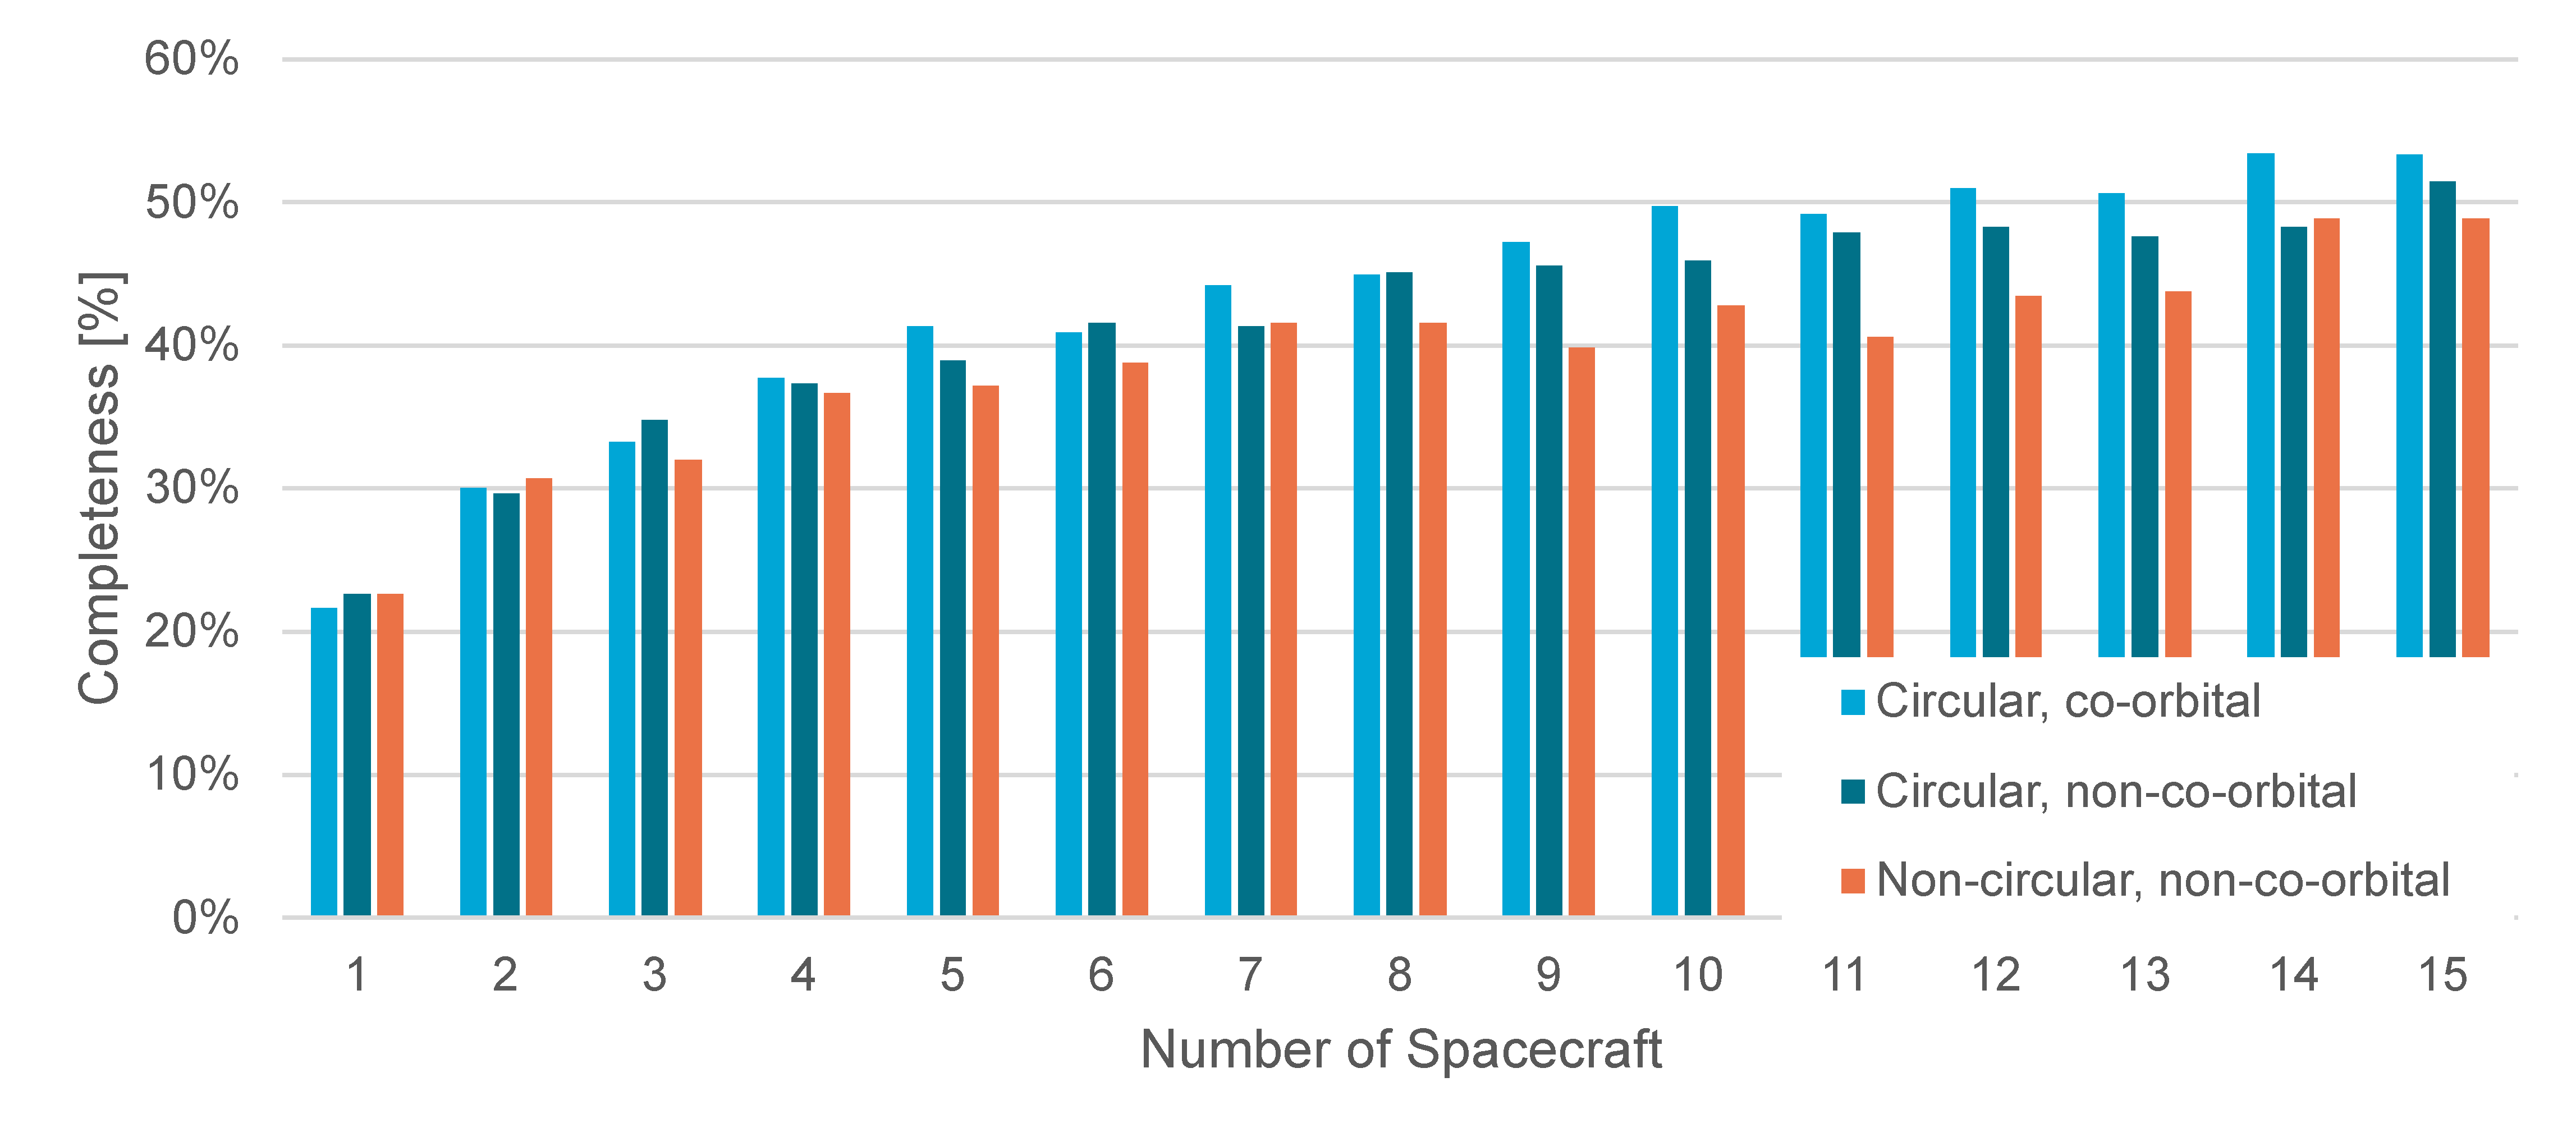
\includegraphics[width=1.0\textwidth]{img/performance_free.pdf}
 \caption{Performances for systems optimized for either a single semi-major axis, distinct semi-major axes and anomalies per spacecraft, or distinct semi-major axes, anomalies and eccentricities per spacecraft.}
 \label{fig:performance_free}
\end{figure}

The results of the optimization processes can be seen in \autoref{fig:performance_free}. It can be seen that several performance breakpoints are present: for low numbers of spacecraft, approximately $1 \leq n \leq 5$, all three methods result in similar performances. Then, for approximately $6 \leq n \leq 10$, the performance of the optimization for the non-circular, non-co-orbital case starts degrading relative to the other two. Lastly, for $n > 10$, the circular, co-orbital solution is superior to the other two methods. These results might be surprising to some readers: one would expect the performance to either increase, or stay equal, as more parameters become available to the optimizer. After all, all solutions found for a circular, co-orbital system of spacecraft (i.e. only a single semi-major axis gets determined by the optimizer), can be recreated by the other two optimizers, and therefore they can reach the same performance. The source of this discrepancy is twofold. The first aspect is the problem of the optimizer overfitting to the noise in the system. The second aspect is related to the actual performance benefits obtainable through these more complex solutions. Although the results here might seem inconclusive, the combination of both aspects will allow supporting the hypothesis presented in the previous section.\\

\begin{figure}[htbp]
 \centering
 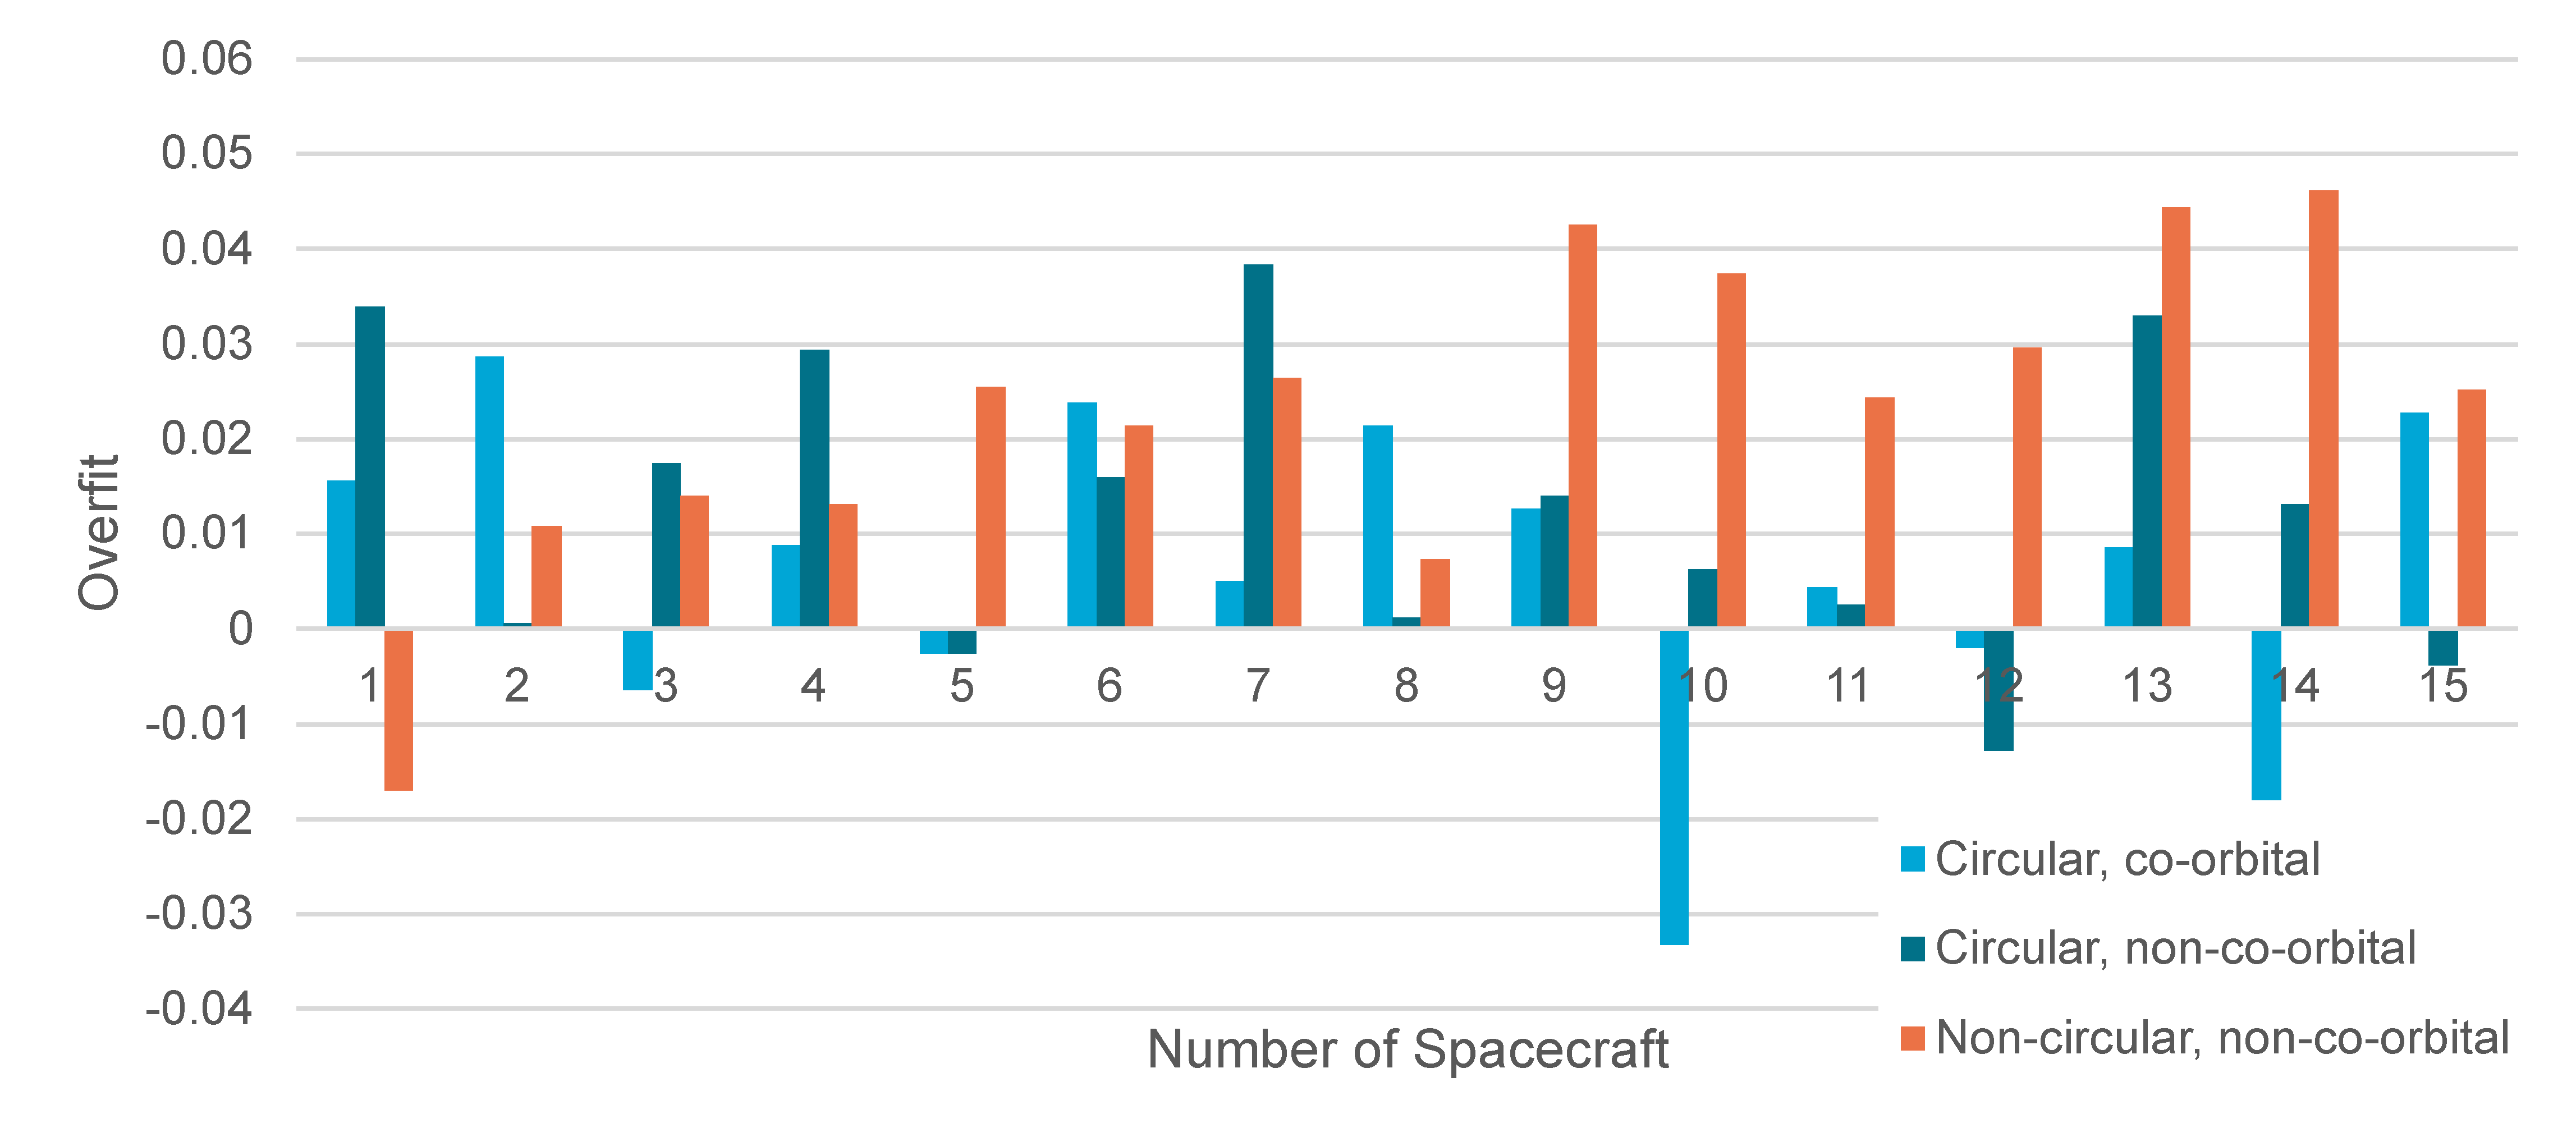
\includegraphics[width=1.0\textwidth]{img/overfit_free.pdf}
 \caption{Overfit of the optimizer per number of spacecraft.}
 \label{fig:overfit_free}
\end{figure}
\begin{figure}[htbp]
 \centering
 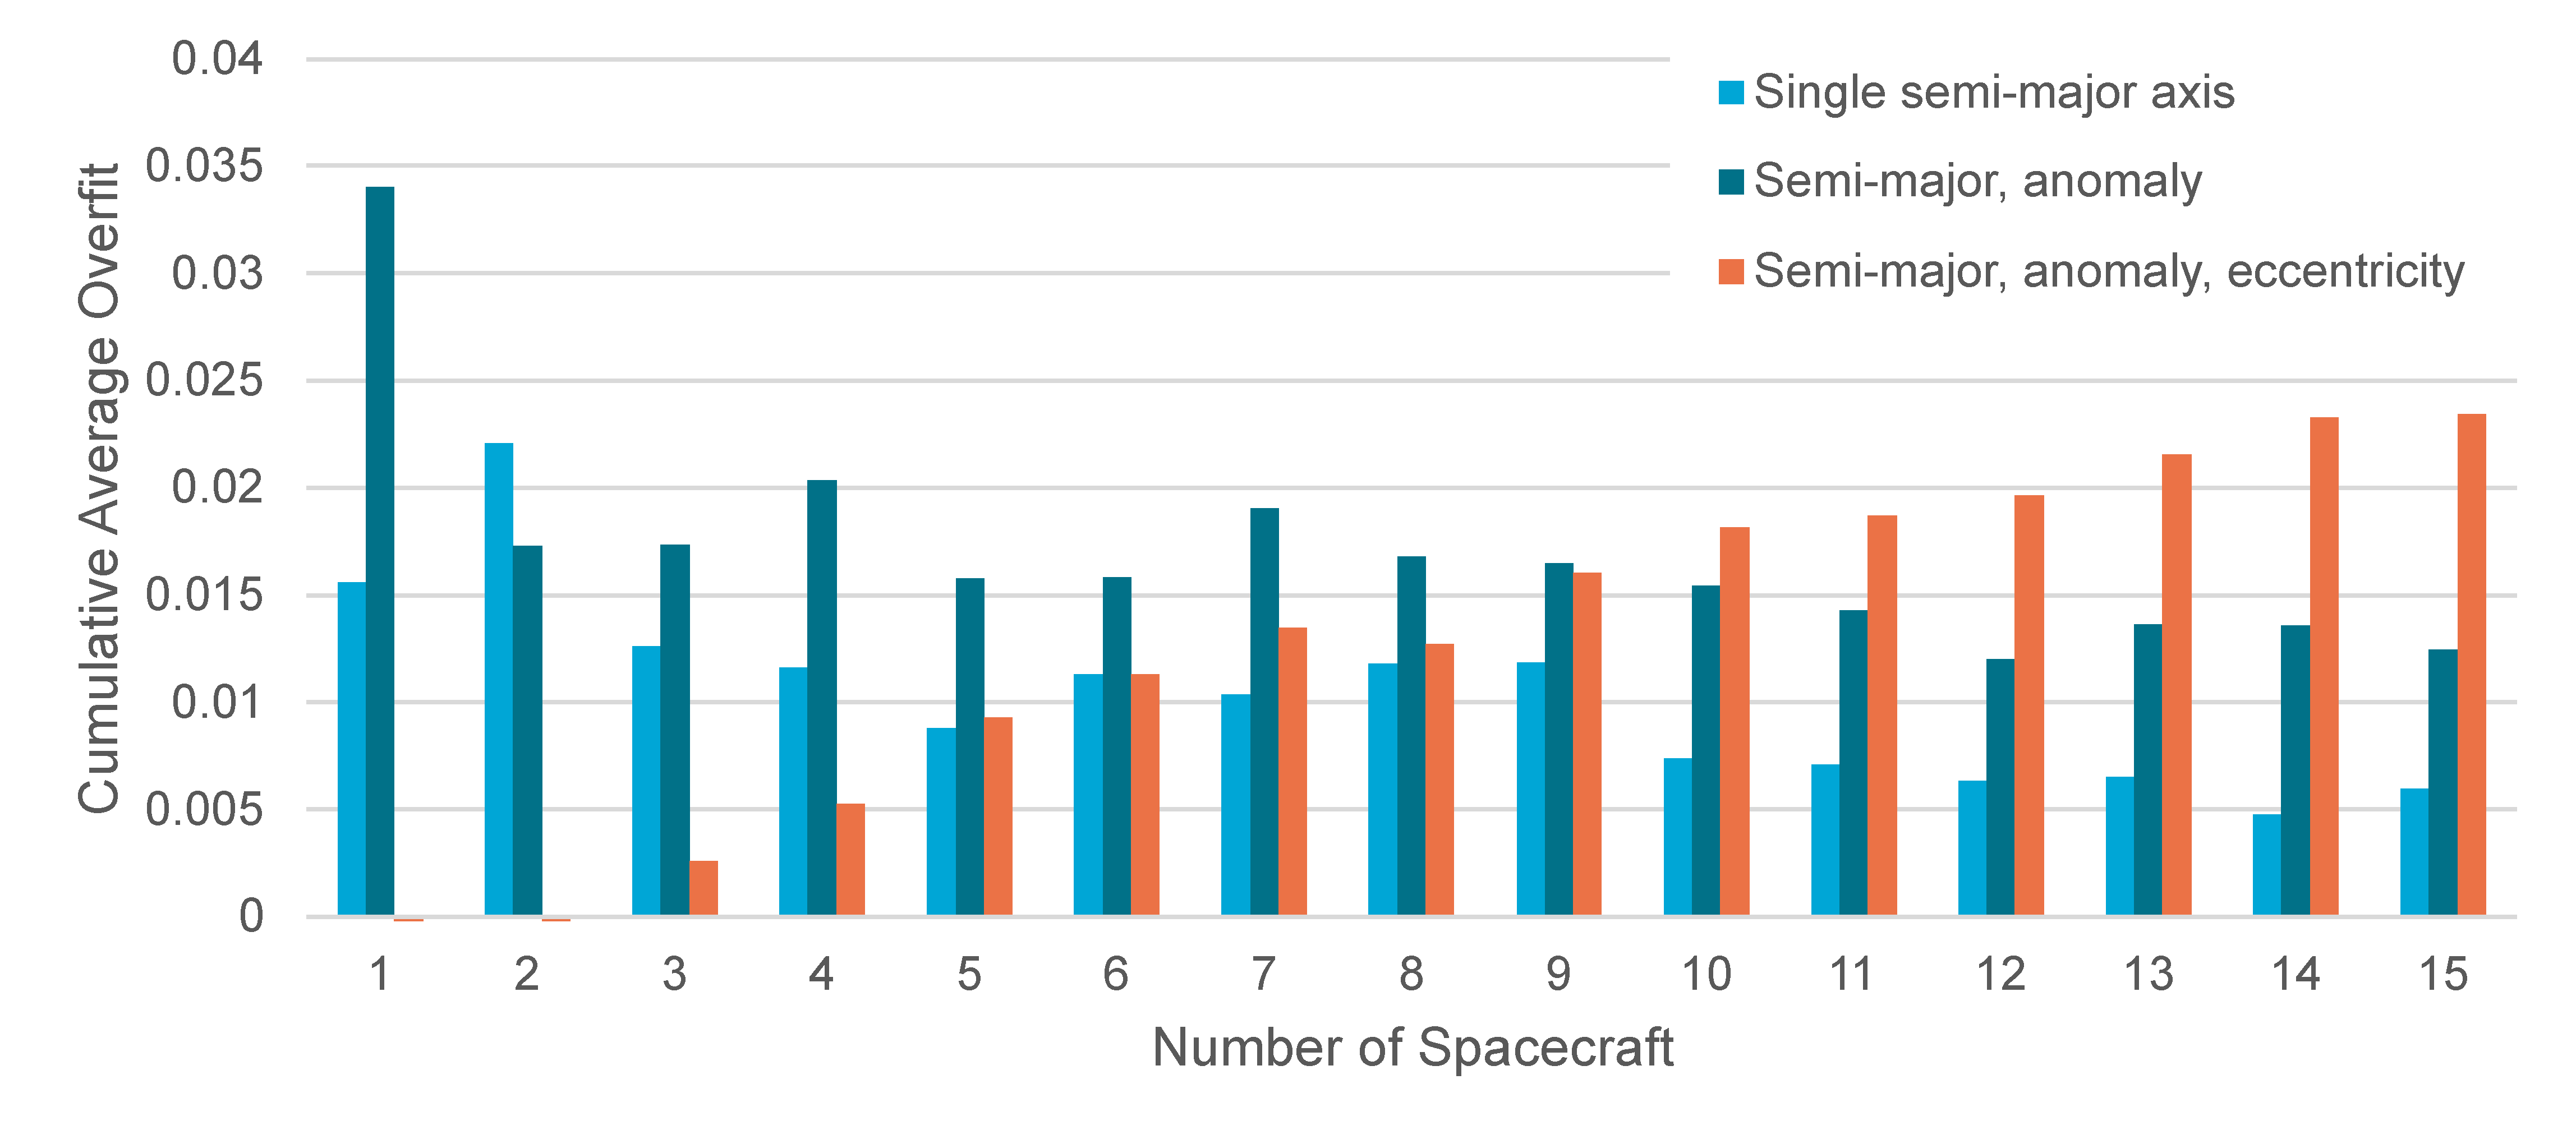
\includegraphics[width=1.0\textwidth]{img/overfit_free_cumulative_average.pdf}
 \caption{Cumulative average of the overfit of the optimizer per number of spacecraft.}
 \label{fig:overfit_free_cumulative_average}
\end{figure}

First, the problem of overfit will be adressed. To illustrate the occurence of overfit at higher dimensionalities, \autoref{fig:overfit_free} gives the overfit for each optimization problem, per spacecraft. Overfit is defined simply as the difference between the learning performance (i.e. the performance predicted by the optimizer for its solution) and the validation performance (the actual performance which can be expected at the solution). As \autoref{fig:overfit_free} is hard to interpret directly, \autoref{fig:overfit_free_cumulative_average} provides the cumulative average up to and including a certain number of spacecraft. Several observations are made here:
\begin{itemize}
 \item As the number of spacecraft increases, the average overfit of the circular, co-orbital system decreases. In other words, for a higher number of spacecraft, the optimizer performs better. This occurs because, in this system, the dimensionality does not increase (as can be seen in \autoref{tab:optimizationcases}, the total number of optimization parameters in this case is always 1), and therefore the task of the optimizer is equally hard. However, as the distribution of spacecraft becomes more uniform, the system will overfit less to the population as the importance of the starting position of each spacecraft becomes smaller: As the population is not exactly radially symmetric, a difference in performance can be expected based on the start position. However, for higher numbers of spacecraft, the variation which is possible with regards to the system becomes smaller, as the angular distance between the spacecraft (and therefore the possible radial asymmetry) is smaller. Therefore, a higher number of spacecraft incurs a regularizing effect on the optimizer.
 \item Secondly, the average overfit of the circular, non-co-orbital system, exhibits no statistically significant slope. The degree of overfit levels out around 1-1.5\%. At this degree of overfitting, the optimizer is capable of finding a solution to the problem.
 \item Lastly, the non-circular, non-co-orbital system shows an \textit{increase} in overfitting. I.e., the optimizer is not capable of keeping up with the increasing dimensionality of the problem, and the quality of the result continually decreases.
\end{itemize}
Before investigating the second point, first some of the solutions of the optimizer will be examined, along with their training progress. Note that in the learning/validation graphs, ``epoch'' refers to the step in the learning process, not the datum of the astronomical coordinate system. The solutions to be investigated are two, six and eleven spacecraft. The one spacecraft case is omitted as the optimal solution is already known from previous analysis to be the optimal solution to the single semi-major axis system. The six and eleven spacecraft cases were chosen as they represent the first solution after the performance breakpoints discussed earlier. Optimization solutions for all numbers of spacecraft investigated, along with the learning/validation curves, can be found in \autoref{ch:appendix}.
\begin{figure}[htbp]
 \centering
 \includegraphics[width=1.0\textwidth]{img/orbits_2.png}
 \caption{Optimization results for systems with two spacecraft.}
 \label{fig:orbits_2}
\end{figure}
\begin{figure}[htbp]
 \centering
 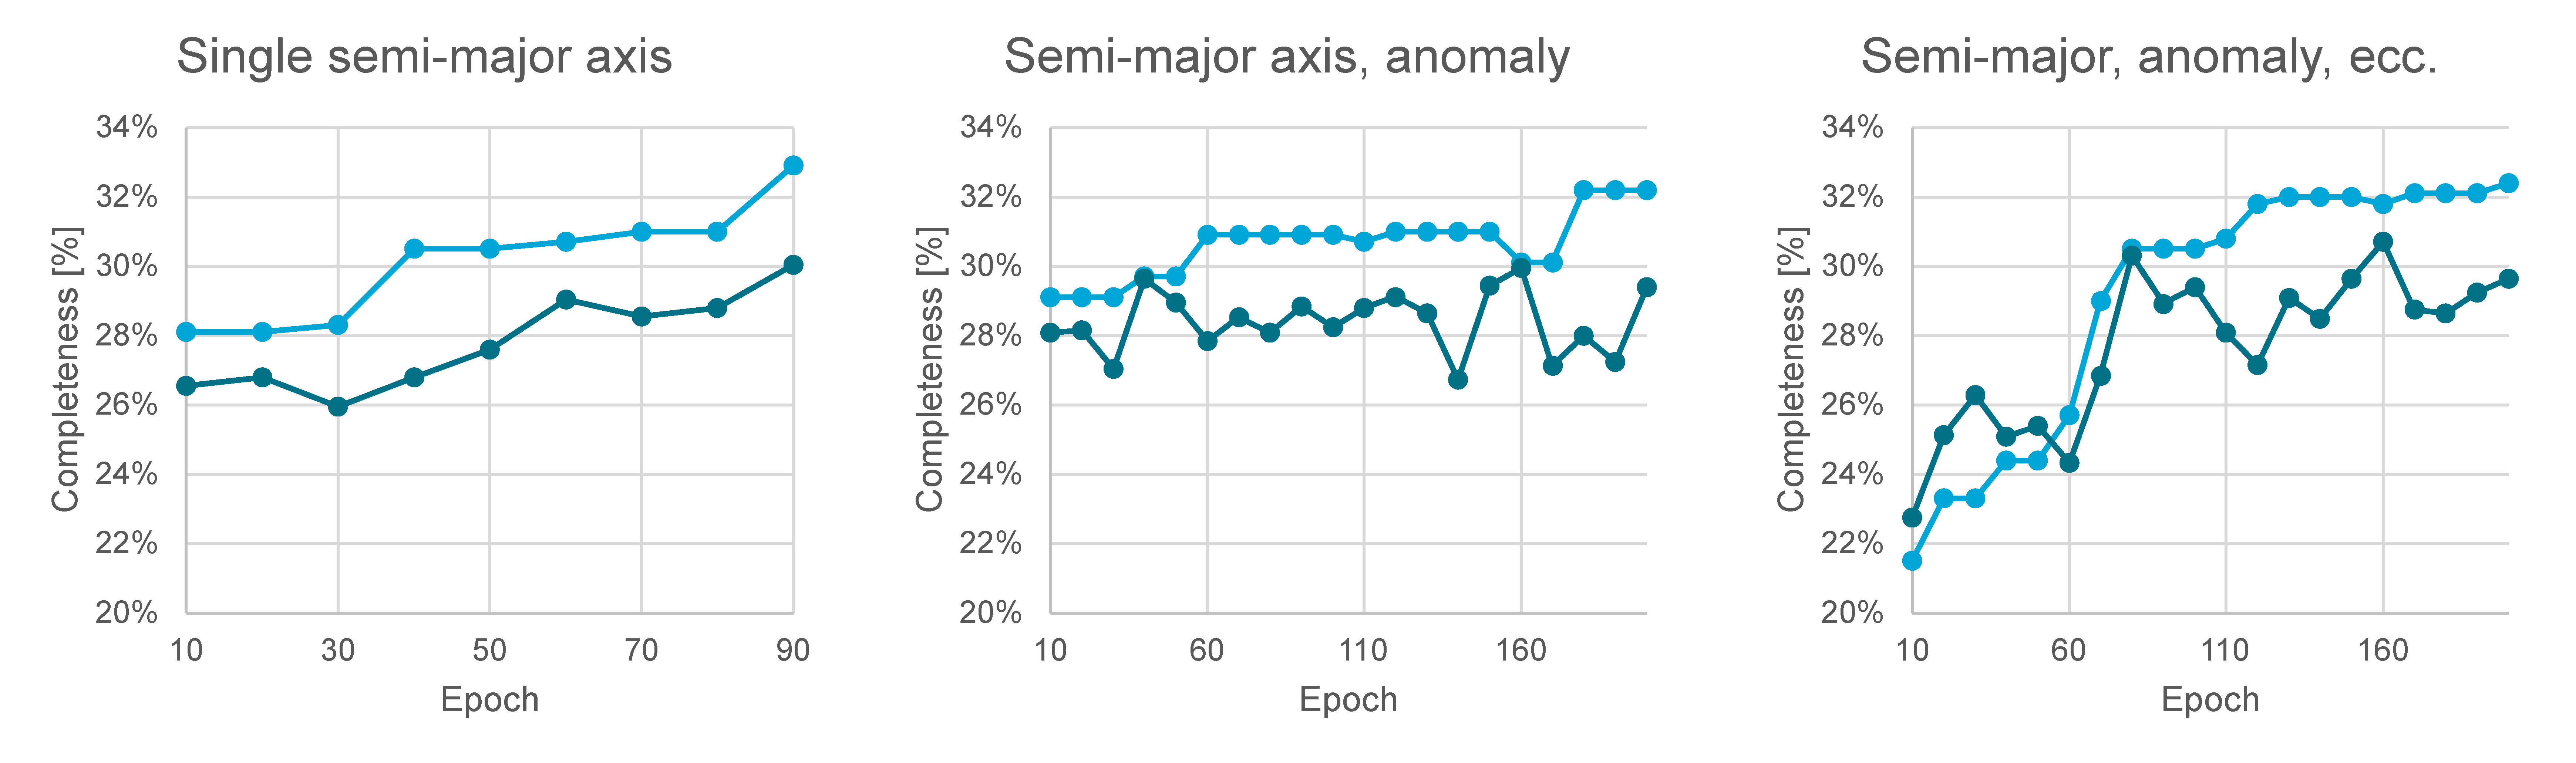
\includegraphics[width=1.0\textwidth]{img/val_orbits_2.pdf}
 \caption{Learning/validation results for systems with two spacecraft.}
 \label{fig:val_orbits_2}
\end{figure}

\begin{table}[htbp]
\centering
\caption{Optimization results for 2 spacecraft.}
\label{tab:opt_2}
\begin{tabulary}{1.0\textwidth}{L|LLL}
                             & $a$   & $e$   & $\theta$ \\ \hline
circular, co-orbital         & 0.922, 0.922 & 0.000, 0.000 & 0.000, 3.142   \\
circular, non-co-orbital     & 0.941, 0.941 & 0.000, 0.000 & 2.486, 2.891   \\
non-circular, non-co-orbital & 1.029, 0.964 & 0.012, 0.100 & 3.609, 3.488  
\end{tabulary}
\end{table}

Firstly, the case for two spacecraft. The solutions and associated learning and validation curves are shown in \autoref{fig:orbits_2} and \autoref{fig:val_orbits_2}. The orbital parameters can be found in \autoref{tab:opt_2}. The circular, co-orbital case can be seen to be optimizing well. The circular, non-co-orbital does place the spacecraft in the same orbit, but closer together. When examining the validation curve, it can be seen that later learning steps do not result in a better validation score, indicating overfitting. This is most likely because the increase in performance from spreading the spacecraft further apart is smaller than the variance in the results. Lastly, the non-circular, non-co-orbital case, which also has access to eccentricity, still behaves well. Instead of a circular solution, one of the spacecraft is placed on a slightly eccentric orbit. This yields a similar performance. In addition, although the optimizer is still well behaved, it takes a large number of steps to reach its eventual solution. \\

\begin{figure}[htbp]
 \centering
 \includegraphics[width=1.0\textwidth]{img/orbits_6.png}
 \caption{Optimization results for systems with six spacecraft.}
 \label{fig:orbits_6}
\end{figure}
\begin{figure}[htbp]
 \centering
 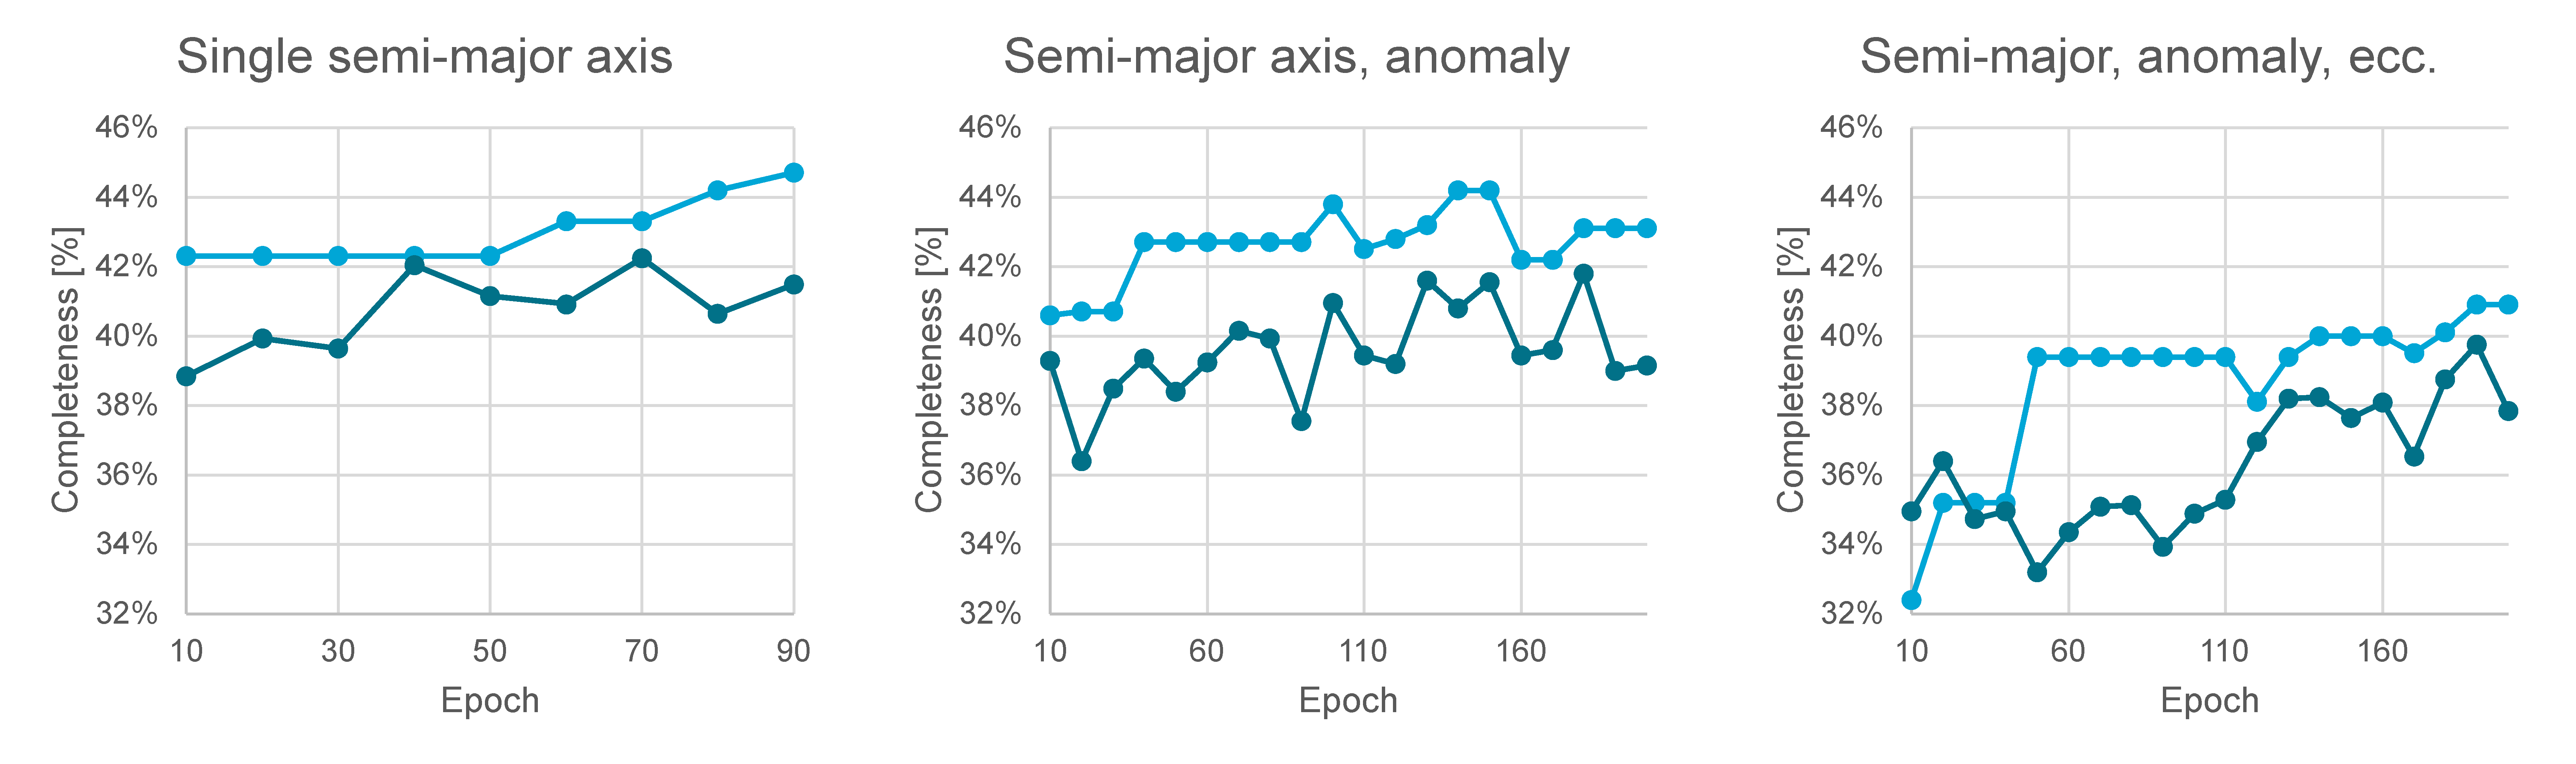
\includegraphics[width=1.0\textwidth]{img/val_orbits_6.pdf}
 \caption{Learning/validation results for systems with six spacecraft.}
 \label{fig:val_orbits_6}
\end{figure}

\begin{table}[htbp]
\centering
\caption{Optimization results for 6 spacecraft.}
\label{tab:opt_6}
\begin{tabulary}{1.0\textwidth}{L|LLL}
                             & $a$                                          & $e$                                          & $\theta$                                      \\ \hline
circular, co-orbital         & 1.170,   1.170, 1.170, 1.170, 1.170, 1.170 & 0.000, 0.000, 0.000, 0.000,   0.000, 0.000 & 0.000, 1.047, 2.094, 3.142,   4.189, 5.236 \\
circular, non-co-orbital     & 1.066,   1.154, 1.104, 1.444, 0.657, 1.510 & 0.000, 0.000, 0.000, 0.000,   0.000, 0.000 & 5.254, 2.511, 1.162, 2.496,   6.469, 2.533 \\
non-circular, non-co-orbital & 0.947,   1.117, 1.156, 0.558, 0.767, 1.194 & 0.051, 0.629, 0.119, 0.562,   0.533, 0.155 & 4.108, 1.860, 0.073, 2.158,   0.811, 5.757
\end{tabulary}
\end{table}

The second case to be examined is the case of six spacecraft. \autoref{fig:orbits_6} and \autoref{fig:val_orbits_6} show the orbits and learning curves, respectively, and \autoref{tab:opt_6} lists the found orbital parameters. As seen in the performance predictions earlier, both circular cases still yield good results for this number of spacecraft, although the non-circular case is starting to underperform. This can be seen in the learning curves. Not only does the non-circular, non-co-orbital system fail to obtain a good solution from the beginning - it's learning performance is also lower than the other two systems - the optimizer struggles to improve the solution through iteration. The resulting orbits provide some insight into what is happening: some of the spacecraft are still in useful positions, however a part is placed on highly eccentric orbits. It has been shown already that these orbits are not a positive addition to the system, and they are most likely the result of overfitting. When considering the circular, non-co-orbital system, interestingly it can be seen that the system still chooses to place some of the spacecraft in the same orbit. However, it also fails to find a solution which outperforms the co-orbital case. \\

\begin{figure}[htbp]
 \centering
 \includegraphics[width=1.0\textwidth]{img/orbits_11.png}
 \caption{Optimization results for systems with eleven spacecraft.}
 \label{fig:orbits_11}
\end{figure}
\begin{figure}[htbp]
 \centering
 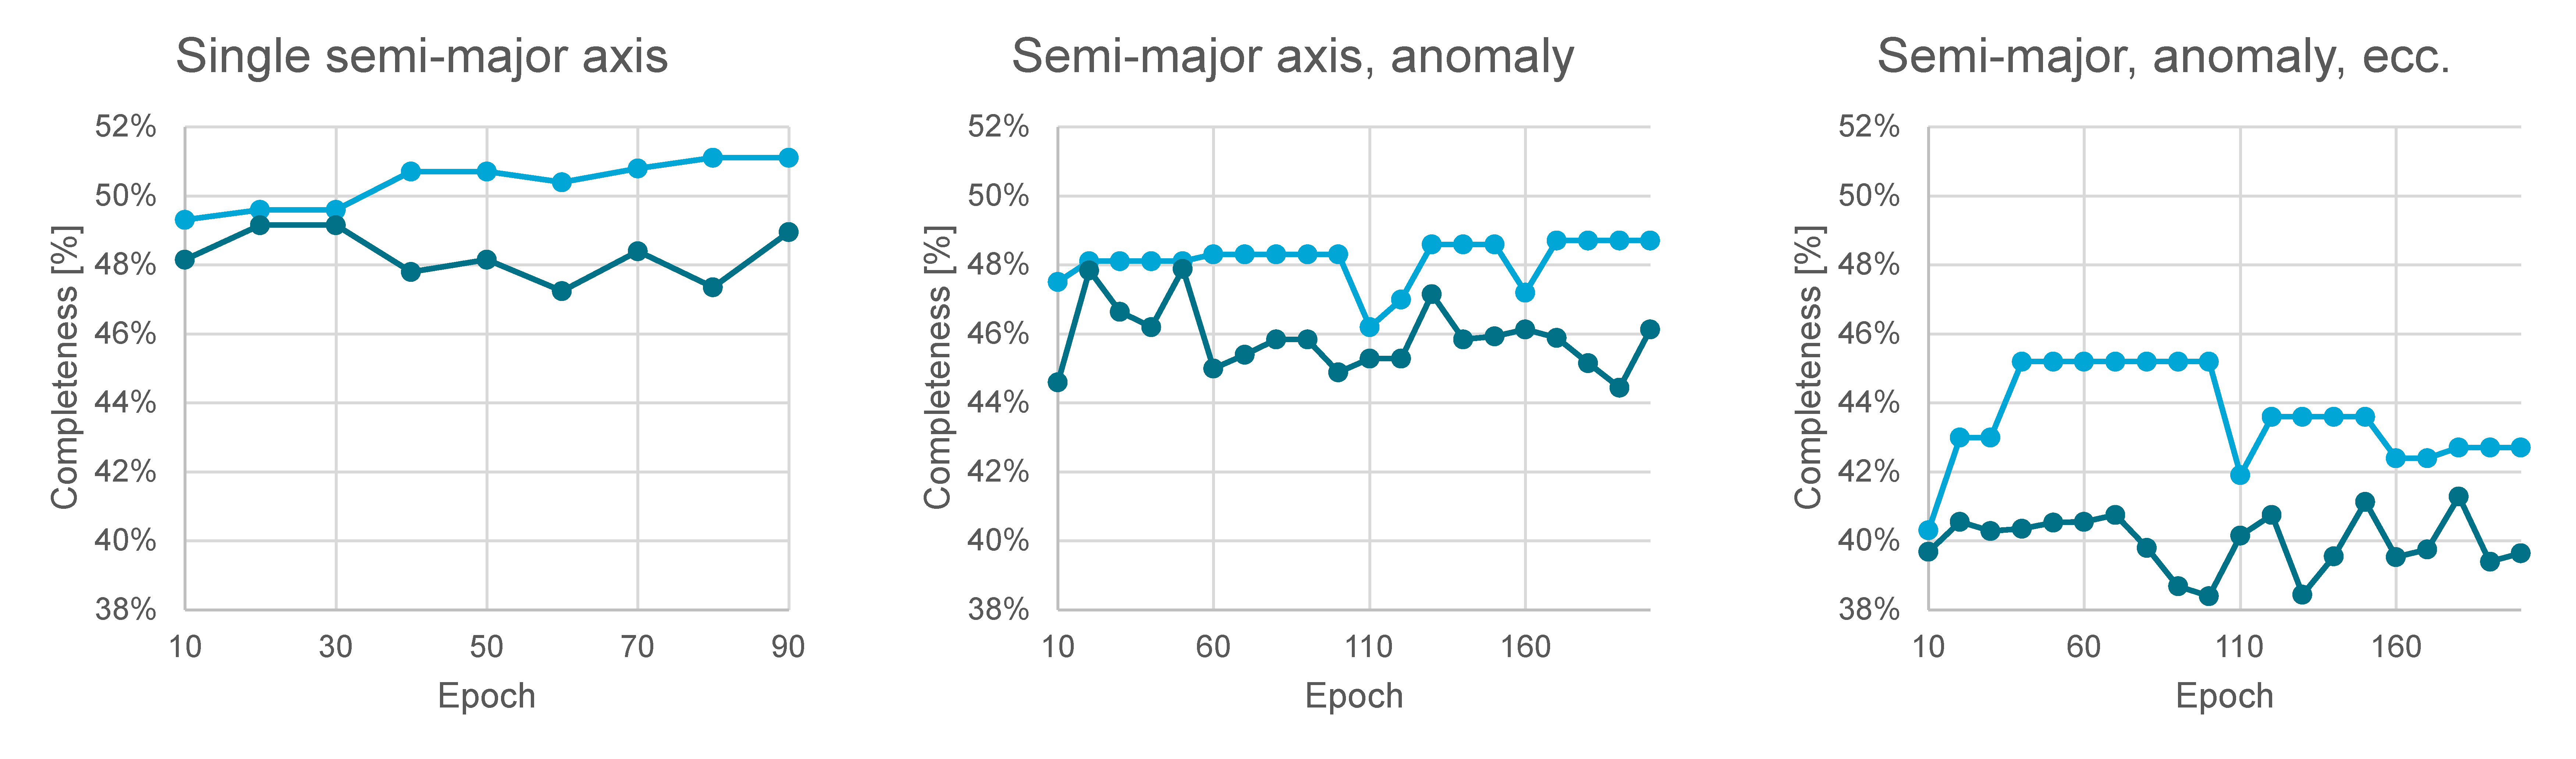
\includegraphics[width=1.0\textwidth]{img/val_orbits_11.pdf}
 \caption{Learning/validation results for systems with eleven spacecraft.}
 \label{fig:val_orbits_11}
\end{figure}

\begin{table}[htbp]
\centering
\caption{Optimization results for 11 spacecraft.}
\label{tab:opt_11}
\begin{tabulary}{1.0\textwidth}{L|LLL}
                             & $a$                                                                                    & $e$                                                                             & $\theta$                                                                         \\ \hline
circular, co-orbital         & 1.443,   1.443, 1.443, 1.443, 1.443, 1.443, 1.443, 1.443, 1.443, 1.443, 1.443        & 0.000, 0.000, 0.000, 0.000,   0.000, 0.000, 0.000, 0.000, 0.000, 0.000, 0.000 & 0.000, 0.571, 1.142, 1.714,   2.285, 2.856, 3.427, 3.998, 4.570, 5.141, 5.712 \\
circular, non-co-orbital     & 0.870,   0.822, 1.220, 1.020, 1.447, 0.480, 0.217, 1.124, 1.714, 1.278, 1.573        & 0.000, 0.000, 0.000, 0.000,   0.000, 0.000, 0.000, 0.000, 0.000, 0.000, 0.000 & 2.062, 4.858, 2.753, 2.168,   2.834, 2.050, 0.609, 5.915, 1.006, 2.057, 2.701 \\
non-circular, non-co-orbital & 1.054,   1.416, 2.065, 1.132, 0.216, 0.191, 0.729, 1.267, 1.100, 1.588, 1.189, 0.248 & 0.190, 0.313, 0.519, 0.683,   0.438, 0.047, 0.817, 0.754, 0.586, 0.084, 0.155 & 2.86, 1.921, 5.046, 4.659,   5.717, 0.094, 4.036, 7.140, 4.715, 6.327        
\end{tabulary}
\end{table}

The last case to be considered is the 11-spacecraft case. The corresponding results can be seen in \autoref{fig:orbits_11}, \autoref{fig:val_orbits_11} and \autoref{tab:opt_11}. The performance of the non-circular system has deteriorated even further: the optimizer loses performance through succesive optimization epochs. In addition the non-co-orbital circular case has also lost good performance. Instead of a well-structured system, the optimizer places the spacecraft in orbits spaced semi-uniformly, and spends significant of effort optimizing the anomaly at epoch. Of course, for a system with differing semi-major axis, the anomaly is a relatively unimportant parameter, and therefore the validation performance can be seen to decrease throughout the process.\\

Clearly, the optimizer is not ideal for obtaining the best solutions across larger dimensionalities. However, an important conclusion can still be drawn from this fact: For lower numbers of spacecraft, the initial performance of the optimizer is still adequate. However, the increase in freedom of placing the spacecraft does in no case yield a statistically significant increase in performance. Recall that the variance in the result when modelling the system is approximately 1-2\%. This then means that no increase in freedom of placing the spacecraft for the region where the optimizer is well-behaved ($n < 11$ for the circular, non-co-orbital case, or $n < 6$ for the non-circular, non-co-orbital case) results in a performance increase of more than 1-2\%. Else, the optimizer would be expected to find this solution at least part of the time. This phenomenon is not inherent to the functioning of the optimizer. It still manifested itself when using a uniform random sampling method, which is more independent of the function to be optimized. However, as mentioned previously, this result is unexpected: to proof that the optimizer functions fully correctly, would require obtaining the same solution for all cases, should the circular, co-orbital case be the best choice. Therefore it can be concluded that for these numbers of spacecraft, a solution in which each spacecraft has its own orbit is probably not statistically superior to a co-orbital solution as alluded to in the previous section, however, problems with the optimizer preclude reaching a definite conclusion on this part. \\

Note that this does not necessarily extrapolate to these solutions \textit{never} being useful. Perhaps research into more complex search strategies, as mentioned previously, could still provide interesting opportunities for such a setup. In addition, it might seem counterintuitive that such a system would not be able to perform better than a system with only a single semi-major axis. Therefore, in the next section, the driving factor behind the systems performance will be investigated.\\


\section{Predicted Performance and Implications for Missions Design}
\label{sec:results_performance}
The last sections treated the reasoning behind the observed performance and how to obtain it. However in addition, it is important to consider what that performance can be expected to be, and how this might affect the design of future NEA survey missions. Therefore, using the optimal solutions found in this chapter, modelling was done to predict what performance might be expected of such a survey. The predictions for performance can be seen in \autoref{fig:performance_prediction}. Here, the projected performance of a system of 1 - 6 spacecraft is shown relative to the current knowledge of the NEA population (per \cite{HarrisPopulation}) and the projected population due to current efforts (as per \cite{2017NEOSDT}). It should be noted that the ``PROJ''-curve relates to the expected completion, in case \textit{no new survey efforts are started}. Comparison of the 1 S/C system in this report, and in \cite{2017NEOSDT} is performed in \autoref{sec:vvperformance}. In addition, the performance relative to the projection is shown in \autoref{fig:performance_prediction_rel}. It can be seen that firstly, any deep space NEA survey will vastly increase the knowledge of the NEA population, increasing the completeness by around 15-20\% at all absolute magnitudes < 20. Additionally, a second spacecraft in the system will yield an additional increase roughly equal in magnitude. After two spacecraft, diminishing returns become a serious factor on the performance. As can be seen in \autoref{fig:performance_prediction_rel}, such systems will still exhibit a sizeable gain in completeness. However, this gain will be centered mostly around the smaller NEAs, i.e., the $21 < H < 24$-range. Note that this follows also from the theory mentioned in the \autoref{sec:results_explanation}: as the number of spacecraft increases, the observable volume for large NEAs barely increases; only an increase among the smaller NEAs is observed (see \autoref{fig:coverage_spread}).\\


\begin{figure}[htbp]
 \centering
 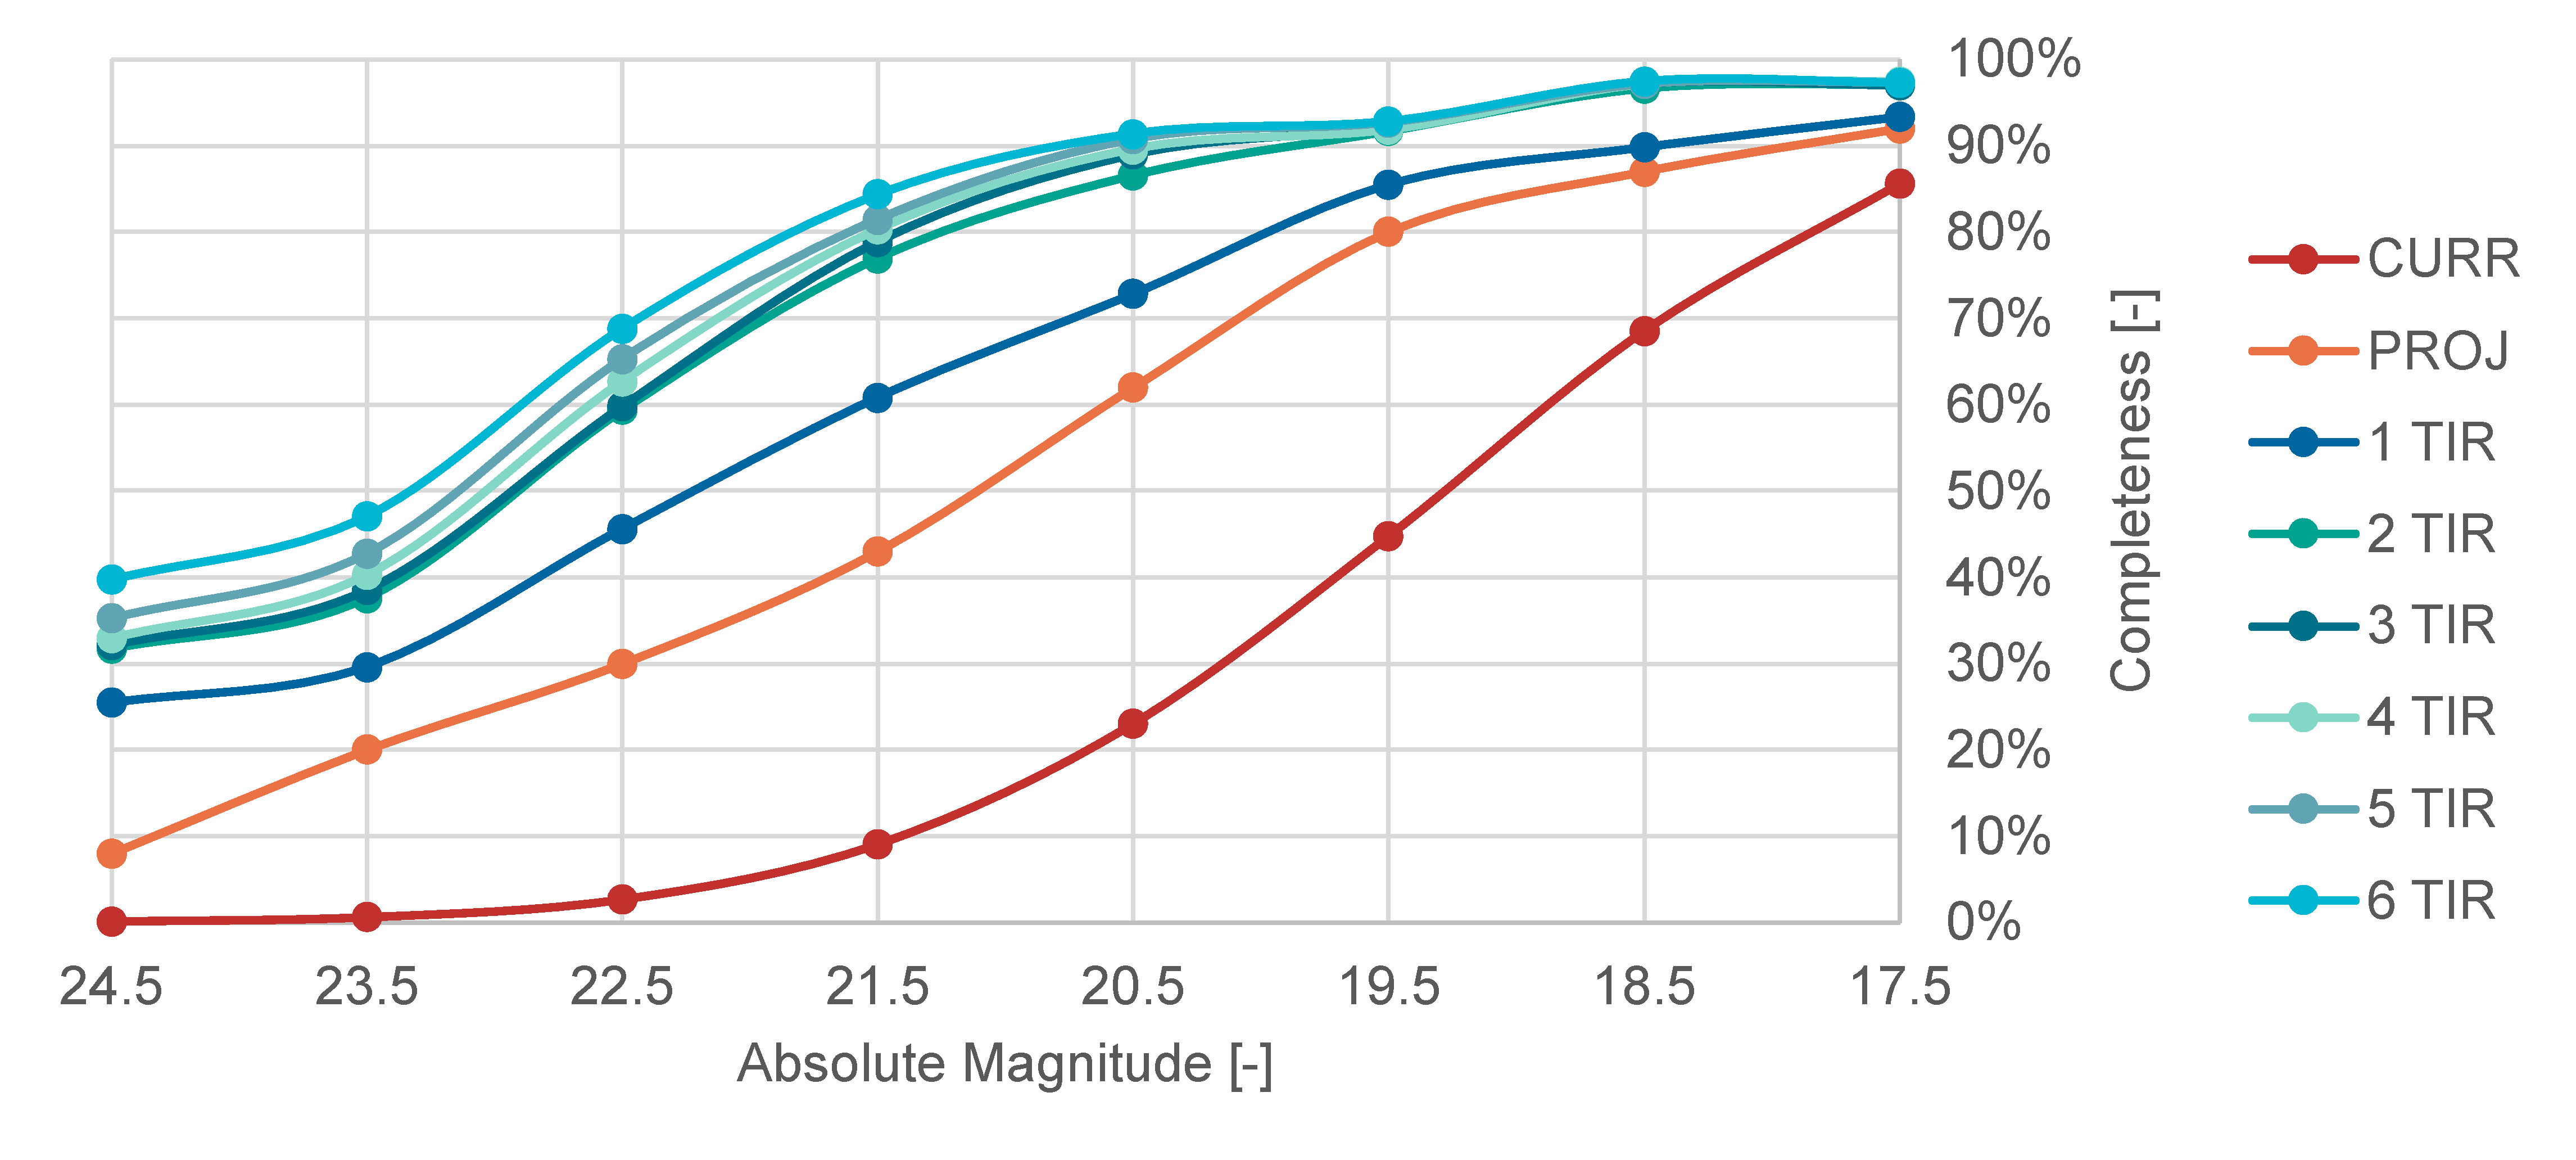
\includegraphics[width=0.9\textwidth]{img/performance_prediction.pdf}
 \caption{Prediction of performance}
 \label{fig:performance_prediction}
\end{figure}

\begin{figure}[htbp]
 \centering
 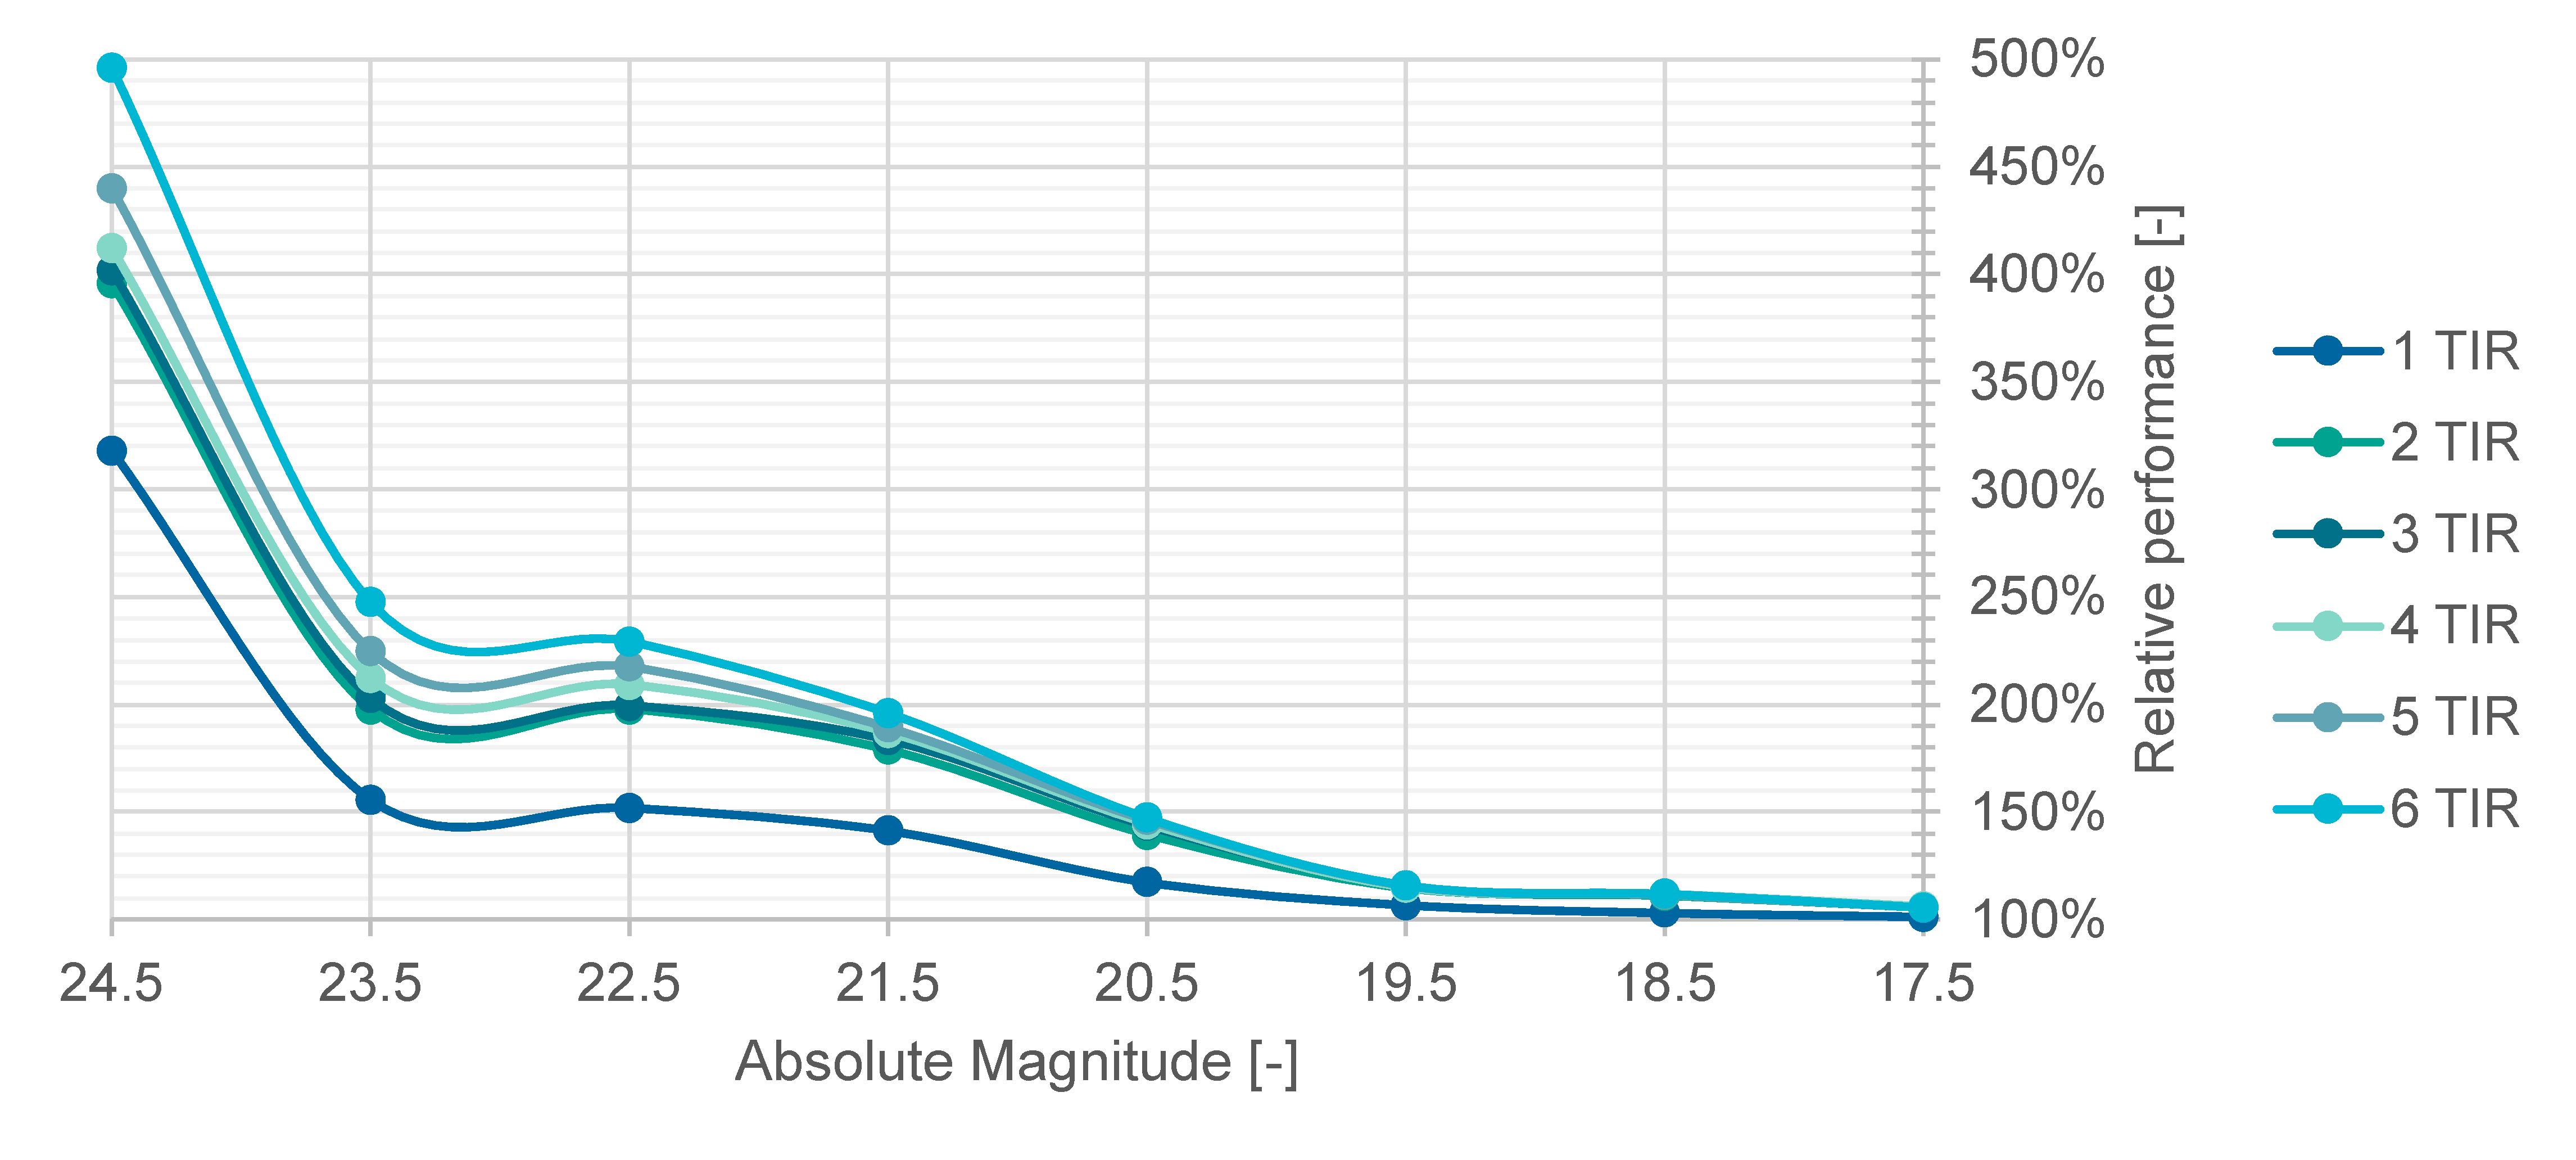
\includegraphics[width=0.9\textwidth]{img/performance_prediction_rel.pdf}
 \caption{Relative prediction of performance}
 \label{fig:performance_prediction_rel}
\end{figure}

Furthermore, a mission designer might be interested in what number of spacecraft would be required to reach a specific level of completeness across the NEA population. Reason for this is that, as seen in the past (e.g. \cite{2003NEOSDT}), objectives are often formulated in terms of a specific completeness level. For this reason, simulations were performed up to 200 spacecraft. The result of this was that the performance follows a roughly logarithmic progression, as can be seen in \autoref{fig:completeness_hypothetical}. Even for extremely large systems of more than 100 spacecraft, completeness nears only 70\%. This occurs as any synergistic benefits of a multi-spacecraft system, as explained in \autoref{sec:researchmultispacecraft} have been obtained at lower numbers of spacecraft already, and higher numbers of spacecraft only provide more frequent imaging capabilities. Therefore, this strong diminishing returns effect is observed. Obviously, such a large system will not be constructed in the near future, and therefore such a goal is seen as unfeasible considering current hardware and software capabilities. Numerically, the relevant values indicate that in order to reach 20\% completeness, 1 spacecraft suffices; for 30\%, a second spacecraft is sufficient. Then, to reach 40\% completeness requires a 6 spacecraft system. 50\% completeness is obtained at 15 spacecraft, 60\% at around 50 spacecraft and lastly, at 200 spacecraft, around 70\% completeness is achieveable. Although not simulated due to practical limitations, it is estimated that around 500 spacecraft would be required to reach 80\% completeness.

\begin{figure}[htbp]
 \centering
 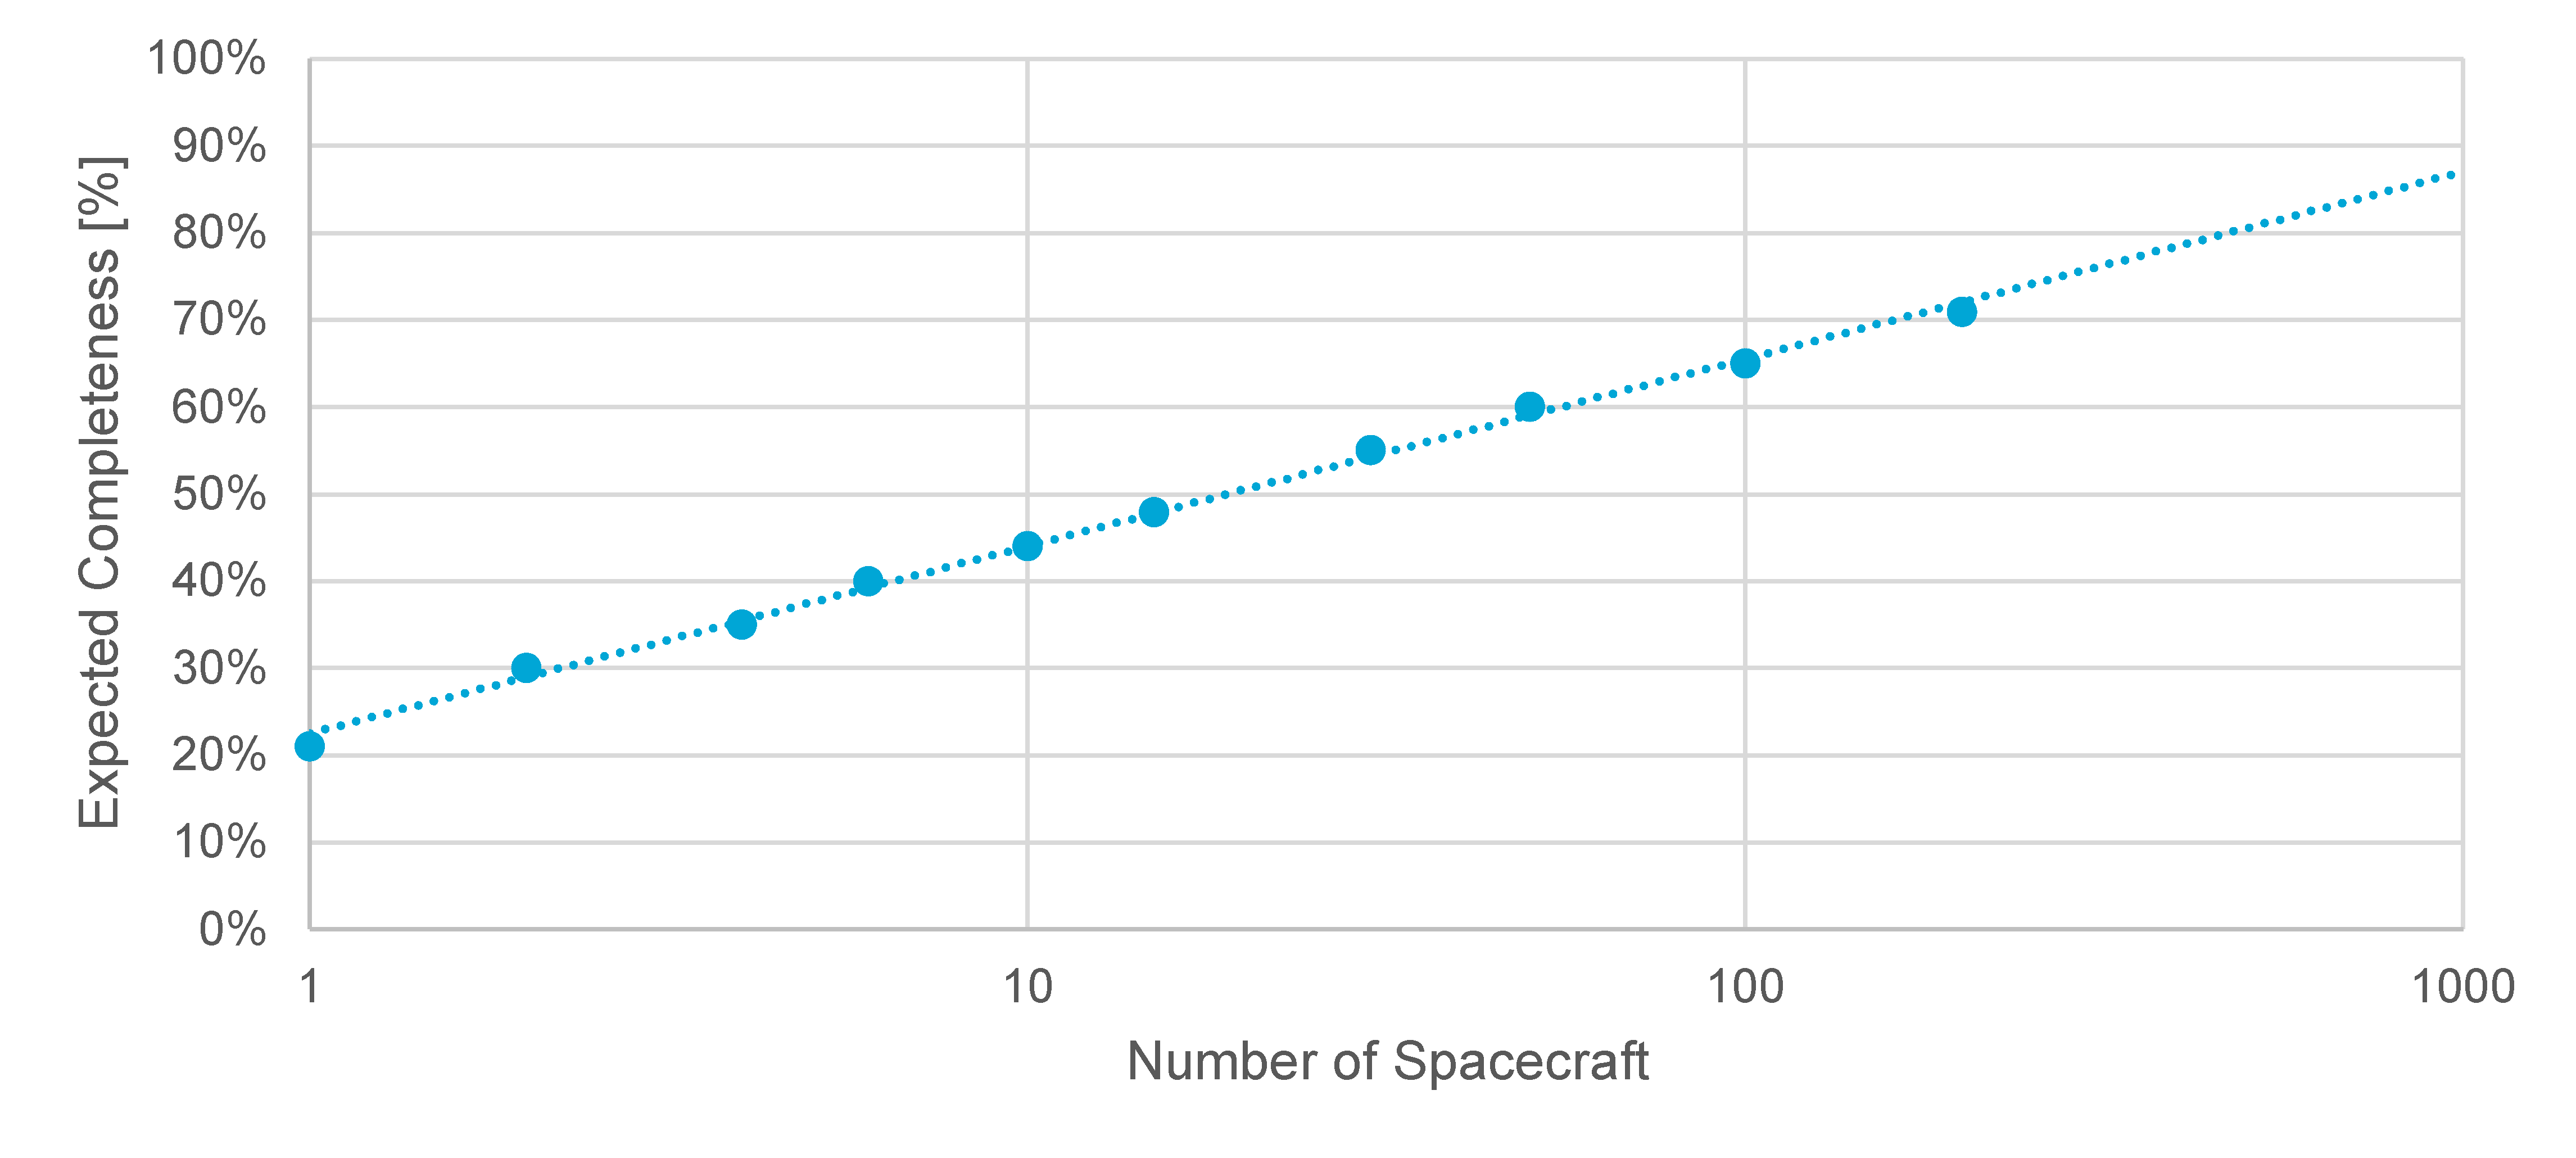
\includegraphics[width=0.8\textwidth]{img/completeness_hypothetical.pdf}
 \caption{Expected performance as a function of number of spacecraft.}
 \label{fig:completeness_hypothetical}
\end{figure}

In conclusion, using currently available search strategies and hardware, optimal solutions can be found by optimizing the system for a single semi-major axis, and spreading out the spacecraft equally throughout the orbit, as this maximizes the observable volume available to the system. The resulting increase of completeness from a single-spacecraft system is around 15-20\% across all NEA sizes smaller than $H=20$. Addition of a second spacecraft raises this performance by a large amount across all NEA sizes, and is defninitely worthy of consideration. Higher numbers of spacecraft only yield small increases in the lower NEA sizes as there is a strong presence of diminishing returns. Lastly, advances in hardware or software technology will be required to feasibly reach higher numbers of completeness in the future, should this be considered. In the next chapter, the accuracy of these results will be examined through the process of verification and validation.
